\documentclass{skripsimathugm}

%-----------------------------------------------------------------
%Disini awal masukan untuk data Skripsi (ISI SESUAI DENGAN DATA ANDA!)
%-----------------------------------------------------------------
\titleind{
Interpolasi Spline Kubik Monoton
}

\titleeng{
Monotone Cubic Spline Interpolation
}

\fullname{Muhammad Fikri Al-Barik}
\NIM{19/442576/PA/19325}
\yearenrollment{2019}
\examdate{26 Juni 2023}
\degree{Sarjana Matematika}
\yearsubmit{2023}
\firstsupervisor{Dr. Sumardi, M.Si.}
\firstexaminer{Prof. Imam Solekhudin, S.Si., M.Si., Ph.D.}
\secondexaminer{Dr. Zenith Purisha, S.Si., M.Sc.}
\thirdexaminer{Hadrian Andradi, S.Si., M.Sc., Ph.D.}

\tolerance=1
\emergencystretch=\maxdimen
\hyphenpenalty=10000
\hbadness=10000

\begin{document}
\cover\titlepage

% \approvalpage
% \declarepage
%Setelah Anda selesai Ujian Akhir Skripsi, scan halaman pengesahan yang telah ditandatangani dosen pembimbing dan penguji, scan juga halaman pernyataan yang telah Anda tandatangani. Selanjutnya simpan hasil scan tersebut dalam bentuk PDF dengan nama pengesahanskripsi.pdf dan pernyataan.pdf (file disimpan di folder yang sama dengan folder dimana file Skripsi.tex tersimpan)
%Hilangkan karakter % sebelum perintah "\approvalpagescan" dan "\declarepage" di bawah ini, dan tambahkan karakter % sebelum perintah "\approvalpage" di atas.
\approvalpagescan
\declarepagescan

%-----------------------------------------------------------------
%Halaman Persembahan (ISI SESUAI DENGAN DATA ANDA!)
%-----------------------------------------------------------------
\acknowledment
\begin{flushright}
\Large\emph\cal{Skripsi ini saya persembahkan untuk \\ayah dan ibu saya tercinta.}
\end{flushright}
%-----------------------------------------------------------------
%-----------------------------------------------------------------


%-----------------------------------------------------------------
%Halaman Motto (ISI SESUAI DENGAN DATA ANDA!)
%-----------------------------------------------------------------
\motto
\emph{"If there is roughness in anything it is bound to disgrace it."}
\begin{flushright}
 Al-Adab Al-Mufrad (466)
\end{flushright}
%-----------------------------------------------------------------
%-----------------------------------------------------------------


%-----------------------------------------------------------------
%Disini awal masukan untuk Prakata (ISI SESUAI DENGAN DATA ANDA!)
%-----------------------------------------------------------------
\preface
% Prakata merupakan pernyataan resmi untuk menyampaikan ucapan terima kasih oleh penulis kepada pihak lain, misalnya kepada para pimpinan institusi, pembimbing, penguji, dan semua pihak yang terkait dalam penyelesaian tugas akhir termasuk orang tua dan penyandang dana. Nama harus ditulis secara lengkap termasuk gelar akademik dan harus dihindari ucapan terima kasih kepada pihak yang tidak terkait. Bahasa yang digunakan harus mengikuti kaidah bahasa Indonesia yang baku.  Prakata diakhiri dengan mencantumkan kota dan tanggal penulisan diikuti di bawahnya dengan kata "Penulis".

% Prakata merupakan pernyataan resmi untuk menyampaikan ucapan terima kasih oleh penulis kepada pihak lain, misalnya kepada para pimpinan institusi, pembimbing, penguji, dan semua pihak yang terkait dalam penyelesaian tugas akhir termasuk orang tua dan penyandang dana. Nama harus ditulis secara lengkap termasuk gelar akademik dan harus dihindari ucapan terima kasih kepada pihak yang tidak terkait. Bahasa yang digunakan harus mengikuti kaidah bahasa Indonesia yang baku.  Prakata diakhiri dengan mencantumkan kota dan tanggal penulisan diikuti di bawahnya dengan kata "Penulis".

Dengan memanjatkan puji dan syukur kehadirat Allah SWT yang telah melimpahkan rahmat, taufik, dan hidayah sehingga penulis dapat menyelesaikan skripsi ini dengan judul "Interpolasi Spline Kubik Monoton", sebagai salah satu syarat untuk memperoleh derajat Sarjana Matematika Program Sarjana Program Studi Matematika Universitas Gadjah Mada.

Penulis menyadari bahwa skripsi ini tidak akan mungkin terselesaikan tanpa adanya dukungan, bantuan, bimbingan, dan nasehat dari berbagai macam pihak selama menyusun skripsi ini. Oleh karena itu, penulis ingin menyampaikan kata terima kasih yang sebesar-besarnya kepada:
\begin{enumerate}
    \item Bapak Prof. Dr.Eng. Kuwat Triyana, M.Si., selaku Dekan Fakultas MIPA.
    \item Bapak Dr. Sumardi, M.Si., selaku dosen pembimbing skripsi atas segala arahan dan masukannya selama penulis menyusun skripsi ini sehingga bisa diselesaikan dengan baik.
    \item Bapak Dr. Budi Surodjo, M.Si., selaku dosen pembimbing akademik atas bimbingannya selama penulis menempuh pembelajaran di Fakultas MIPA Universitas Gadjah Mada.
    \item Seluruh staff pengajar Fakultas MIPA yang telah memberi ilmu yang tak ternilai selama penulis menempuh pembelajaran di Fakultas MIPA Universitas Gadjah Mada.
    \item Kedua orang tua penulis, Noziandra dan Lisnamidyani, yang selalu memberi kasih sayang, doa, dan nasihat, serta selalu sabar dalam menghadapi penulis selama ini. Penulis berharap bisa menjadi sosok yang diharapkan oleh kedua orang tua penulis.
    \item Kakek dan nenek penulis yang telah ikut berperan dalam membesarkan penulis menjadi sebagai mana penulis sekarang.
    \item Kakak dan adik penulis yang telah ikut mendukung penulis selama ini.
    \item Teman-teman matemasika angkatan 2019 yang telah membantu penulis selama menempun pembelajaran di Fakultas MIPA Universitas Gadjah Mada.
    \item Staff preksu yang telah menolong penulis selama ada di Jogja, terutama pada hari senin dan kamis.
    \item Semua pihak yang tidak bisa penulis sebut satu per satu, yang telah memberikan doa sehingga dapat terselasaikannya skripsi ini.
\end{enumerate}

Penulis menyadari bahwa di dalam skripsi ini masih banyak kekurangan, untuk itu penulis sangat mengharapkan kritik dan sarang yang bersifat membangun. Penulis berharap skripsi ini dapat bermanfaat.
\vspace{0.8cm}

\begin{tabular}{p{7cm}c}
&Yogyakarta, 2 Agustus 2023\\
&\\
&\\
&Muhammad Fikri Al-Barik
\end{tabular}
%-----------------------------------------------------------------
%-----------------------------------------------------------------


%-----------------------------------------------------------------
%Daftar Isi (TIDAK PERLU DIUBAH)
%-----------------------------------------------------------------
\newpage\phantomsection\addcontentsline{toc}{chapter}{DAFTAR ISI}
\makeatletter\renewcommand\l@chapter[2]{\ifnum \c@tocdepth >\z@\addpenalty\@secpenalty\addvspace{0em}\setlength\@tempdima{1.4em}\begingroup\parindent \z@ \rightskip \@pnumwidth\parfillskip -\@pnumwidth\leavevmode \bfseries\advance\leftskip\@tempdima\hskip -\leftskip#1\nobreak\ \leaders\hbox{$\m@th\mkern \@dotsep mu\hbox{.}\mkern \@dotsep mu$}\hfil\nobreak\hb@xt@\@pnumwidth{\hss #2}\par\endgroup\fi}\makeatother
\begin{singlespacing}\tableofcontents\end{singlespacing}
%-----------------------------------------------------------------
%-----------------------------------------------------------------

%-----------------------------------------------------------------
%Daftar Tabel (JIKA DIPERLUKAN, HAPUS KARAKTER % SEBELUM \newpage dan \begin)
%-----------------------------------------------------------------
\newpage\phantomsection\addcontentsline{toc}{chapter}{DAFTAR TABEL}
\begin{singlespacing}\listoftables\end{singlespacing}
%-----------------------------------------------------------------
%-----------------------------------------------------------------

%-----------------------------------------------------------------
%Daftar Gambar (JIKA DIPERLUKAN, HAPUS KARAKTER % SEBELUM \newpage dan \begin)
%-----------------------------------------------------------------
\newpage\phantomsection\addcontentsline{toc}{chapter}{DAFTAR GAMBAR}
\begin{singlespacing}\listoffigures\end{singlespacing}
%-----------------------------------------------------------------
%-----------------------------------------------------------------


%-----------------------------------------------------------------
%Daftar Lambang (ISI SESUAI DENGAN DATA ANDA!)
%-----------------------------------------------------------------
\lambang
\begin{tabular}{cp{10.5cm}}
    $x\in A$ & : $x$ adalah anggota dari himpunan $A$\\
    $\R$ & : himpunan bilangan real\\
    $\Leftrightarrow$ & : jika dan hanya jika \\
    $\Rightarrow$ & : jika maka\\
    $\Sigma$ & : jumlahan seluruhnya \\
    $\blacksquare$ & : akhir dari bukti \\
    $\Pi$ & : perkalian seluruhnya\\
    $sign(x)$ & : tanda dari bilangan real $x$\\
    $C^n$ & : himpunan fungsi yang memiliki $n$ turunan kontinu\\
    $||v||_\infty$ & : $\max(|v_1|,|v_2|,\dots,|v_n|)$\\
    $f_i$ & : $f(x_i)$ \\
    $\dot{f}_i$ & : pendekatan turunan $f$ di titik $x_i$\\
    $\lambda_i$ & : $\frac{h_{i+1}}{h_i+h_{i+1}}$\\
    $\dot{f_i}$ & : $f'(x_i)$\\
    $\mu_i$ & : $\frac{h_i}{h_i+h_{i+1}}$\\
    $h_i$ & : $x_{i+1}-x_i$\\
    $\alpha_i$ & : $\frac{\dot{f_i}}{m_i}$\\
    $\hat{h}$ & : $\max(h_0,\dots,h_{n-1})$\\
    $\beta_i$ & : $\frac{\dot{f_{i+1}}}{m_i}$\\
    $m_i$ & : $\frac{f_{i+1}-f_i}{h_i}$\\
    $\mathcal{H} \{x_0,\dots,x_n\}$ & : $[\max(x_0,\dots,x_n),\min(x_0,\dots,x_n)]$
\end{tabular}

%-----------------------------------------------------------------
%-----------------------------------------------------------------


%-----------------------------------------------------------------
%Disini awal masukan Intisari (ISI SESUAI DENGAN DATA ANDA!)
%-----------------------------------------------------------------
\begin{abstractind}
% Intisari Intisari Intisari Intisari Intisari Intisari Intisari Intisari Intisari Intisari Intisari Intisari Intisari Intisari Intisari Intisari Intisari Intisari Intisari Intisari Intisari Intisari Intisari Intisari Intisari Intisari Intisari Intisari Intisari Intisari Intisari Intisari Intisari Intisari Intisari Intisari Intisari Intisari Intisari Intisari Intisari Intisari Intisari Intisari Intisari Intisari Intisari Intisari Intisari Intisari Intisari Intisari Intisari Intisari Intisari Intisari Intisari Intisari Intisari.
Metode interpolasi spline kubik adalah metode interpolasi yang menghasilkan interpolasi dengan regularitas $C^2$. Pada umumnya, polinomial hasil interpolasi spline kubik belum tentu memiliki sifat monoton. Hasil interpolasi yang tidak monoton dapat mengakibatkan turunnya akurasi dikarenakan adanya osilasi pada hasil interpolasi. Osilasi dapat terjadi ketika dilakukan interpolasi pada fungsi yang tidak kontinu. Pada penelitian ini dikaji metode interpolasi bersifat monoton untuk mengatasi turunnya akurasi ketika menginterpolasi fungsi yang tidak kontinu.
% Pada hasil interpolasi di sekitar titik tidak kontinu dapat terjadi osilasi dikarenakan fenomena Gibbs yang mengakibatkan menurunnya akurasi di sekitar titik tersebut. Pada penelitian ini dikaji metode interpolasi yang menghasilkan interpolasi bersifat monoton untuk mengatasi turunnya akurasi ketika menginterpolasi fungsi yang memiliki titik tidak kontinu.

\end{abstractind}
%-----------------------------------------------------------------
%-----------------------------------------------------------------

%-----------------------------------------------------------------
%Disini awal masukan untuk Abstract (ISI SESUAI DENGAN DATA ANDA!)
%-----------------------------------------------------------------
\begin{abstracteng}
% Abstract Abstract Abstract Abstract Abstract Abstract Abstract Abstract Abstract Abstract Abstract Abstract Abstract Abstract Abstract Abstract Abstract Abstract Abstract Abstract Abstract Abstract Abstract Abstract Abstract Abstract Abstract Abstract Abstract Abstract Abstract Abstract Abstract Abstract Abstract Abstract Abstract Abstract Abstract Abstract Abstract Abstract Abstract Abstract Abstract Abstract Abstract Abstract Abstract Abstract Abstract Abstract Abstract Abstract Abstract Abstract Abstract Abstract Abstract.
The cubic spline interpolation method is an interpolation method that produces an interpolation with $C^2$ regularity. In general, polynomials resulting from cubic spline interpolation do not necessarily have monotone properties. Interpolation results that are not monotonous can result in decreased accuracy due to oscillations in the interpolation results. Oscillations can occur when interpolating a function that is not continuous. In this research, the monotone interpolation method is studied to overcome the decrease in accuracy when interpolating discontinuous functions.
\end{abstracteng}
%-----------------------------------------------------------------
%-----------------------------------------------------------------

%-----------------------------------------------------------------
%Disini awal masukan untuk Bab (ISI BAB I DAPAT DIEDIT DI FILE Bab1.tex,
%ISI BAB II DAPAT DIEDIT DI FILE Bab2.tex, dst...)
%-----------------------------------------------------------------
\chapter{PENDAHULUAN}
\section{Latar Belakang Masalah}
% Penulisan latar belakang dan permasalahan disajikan dalam bentuk uraian yang secara kronologis diarahkan untuk langsung menuju rumusan masalah. Dalam latar belakang dan permasalahan dapat dimasukkan   beberapa   uraian   singkat   penelitian  terdahulu   yang   dapat   memperkuat   alasan   mengapa penelitian ini dilakukan. Apabila diperlukan, pada bagian ini dimungkinkan memuat hipotesis/dugaan secara umum.

Metode interpolasi adalah metode numerik untuk menyisipkan titik baru di antara titik yang diberikan. Sebelumnya, penelitian terkait metode interpolasi telah dilakukan dalam karya \tpustaka{boor} yang meneliti tentang interpolasi polinomial secara sepotong-sepotong. Interpolasi polinomial secara sepotong-sepotong dikenal juga sebagai interpolasi spline. Pada umumnya metode interpolasi spline menghasilkan polinomial interpolasi dengan derajat yang lebih kecil dibandingkan interpolasi polinomial lainnya.

Metode interpolasi spline kubik adalah salah satu interpolasi spline yang menghasilkan polinomial sepotong-sepotong dengan derajat kurang dari empat. Interpolasi spline kubik memiliki kekurangan pada hasil interpolasinya, yaitu hasil interpolasi belum tentu memiliki sifat monoton.

Metode interpolasi digunakan dengan mempertimbangkan bagaimana sifat interpolasi yang dihasilkan. Salah satu sifat hasil interpolasi yang ingin dipertahankan adalah sifat monoton. Sifat monoton ingin dipertahankan dalam interpolasi, terutama jika data yang diberikan monoton. Dalam penelitian \tpustaka{fritsch} diteliti syarat-syarat cukup pada turunan pertama di titik-titik yang diberikan sehingga polinomial hasil interpolasi Hermite kubik memiliki sifat monoton.

Berdasarkan hal tersebut dibentuk rumusan masalah dari skripsi ini, yaitu:
\begin{enumerate}
    \item Apakah dapat dibentuk interpolasi spline kubik yang monoton?
    \item Bagaimana tingkat akurasi dari interpolasi spline kubik yang monoton?
\end{enumerate}



\section{Tujuan dan Manfaat Penelitian}
% Tujuan penelitian berisikan penjelasan secara spesifik tentang hal-hal yang ingin dicapai melalui penelitian yang dilakukan. Manfaat yang diperoleh dari penelitian guna memberi penjelasan kemanfaatan bagi pengembangan penelitian atau aplikasinya.

Tujuan penelitian ini dilakukan adalah sebagai berikut:
\begin{enumerate}
    \item Membentuk syarat cukup interpolasi Hermite kubik monoton.
    \item Meneliti tingkat akurasi interpolasi Hermite kubik dengan turunan numerik sebagai pendekatan turunan pertama.
    \item Membentuk metode spline kubik berbasis polinomial Hermite kubik sehingga syarat cukup agar interpolasi Hermite kubik menghasilkan interpolasi yang monoton juga berlaku pada interpolasi spline kubik yang dibentuk.
    \item Meneliti tingkat akurasi interpolasi apline kubik monoton yang dibentuk.
    \item Memberikan metode interpolasi alternatif, ketika metode interpolasi spline kubik tidak memenuhi syarat cukup untuk memperoleh interpolasi yang monoton.
    \item Meneliti tingkat akurasi metode interpolasi alternatif spline kubik monoton.
\end{enumerate}

Metode interpolasi yang monoton bermanfaat dalam menginterpolasi fungsi yang tidak kontinu atau memiliki gradien yang sangat besar sehingga grafiknya sangat curam pada suatu titik. pada umumnya fungsi tidak kontinu yang diinterpolasi secara spline mengalami osilasi di sekitar titik tidak kontinu. Hal ini menyebabkan hasil interpolasi menjadi tidak akurat di sekitar titik tidak kontinu. Metode interpolasi monoton juga bermanfaat dalam menginterpolasi data yang monoton sehingga sifat monotonnya dapat dipertahankan.

\section{Tinjauan Pustaka}
% Tinjauan pustaka memuat uraian sistematis tentang informasi hasil penelitian yang disajikan dalam pustaka   dan   menghubungkannya   dengan   masalah   penelitian   yang   sedang   diteliti.   Fakta-fakta  yang dikemukakan sejauh mungkin diacu dari sumber aslinya, dengan mengikuti cara sitasi nama dan tahun dalam kurung biasa.

% Berikut ini merupakan contoh penulisan citation: \tpustaka{buc}.

Persamaan linear adalah sebuah persamaan yang melibatkan jumlahan $n$ buah variabel tanpa ada perkalian antar variabelnya. Sejumlah persamaan linear dengan variabel yang sama dapat membentuk sebuah sistem persamaan linear yang ketika diselesaikan bisa saja memiliki solusi tunggal, tak berhingga, atau bahkan solusinya tidak ada. Matriks adalah rangkaian angka yang membentuk sebuah persegi panjang yang elemen-elemennya menempati sebuah baris dalam kolom tertentu. Penjabaran lebih lanjut terkait sistem persamaan linear, matriks, dan vektor diambil dari buku karya \tpustaka{howard} dan \tpustaka{olver}.

Fungsi merupakan sebuah pemetaan dari suatu himpunan ke himpunan lain. Salah satu contoh fungsi pada himpunan bilangan real di antaranya adalah fungsi polinomial. Fungsi polinomial pada suatu interval merupakan fungsi kontinu. Turunan fungsi adalah pengukuran terkait perubahan nilai fungsi berdasarkan nilai inputnya. Penjabaran tentang sifat-sifat dari fungsi kontinu dan turunan fungsi diambil dari buku karya \tpustaka{bartle} dan \tpustaka{thomas}.

Metode interpolasi merupakan metode untuk menemukan fungsi untuk menysipkan titik baru di antara titik yang diberikan. Metode interpolasi yang menghasilkan fungsi polinomial disebut sebagai interpolasi polinomial. Ada banyak sekali metode interpolasi polinomial di antaranya adalah metode interpolasi Hermite, spline kubik, dan beda bagi. Pada penelitian ini, akan diteliti tentang pengembangan dari metode spline kubik. Dalam pengembangan metode tersebut, diambil referensi tentang sifat metode interpolasinya dari buku karya \tpustaka{burden}, \tpustaka{boor}, dan \tpustaka{atkinson}.

Dalam proses interpolasi titik terkadang ada sifat khusus dari titik-titik yang ingin kita pertahankan, salah satunya adalah sifat kemonotonan. Interpolasi monoton merupakan metode interpolasi yang bertujuan untuk mempertahankan kemonotonan titik yang diinterpolasi. Selain untuk mempertahankan kemonotonan titik yang kita interpolasikan, interpolasi monoton juga bermanfaat untuk membatasi hasil interpolasi sehingga tidak terjadi osilasi. Hal ini dijelaskan pada halaman yang ditulis \tpustaka{bird}.

Interpolasi Hermite kubik merupakan interpolasi yang membagi data menjadi interval-interval tertentu sehingga derajat dari polinomial hasil interpolasi datanya menjadi tidak terlalu besar. Interpolasi Hermite kubik dapat memiliki sifat monoton dengan memberikan syarat-syarat tambahan. Syarat-syarat tambahan ini dijelaskan pada jurnal \tpustaka{fritsch}.

Pada \tpustaka{aràndiga} dijelaskan bagaimana membentuk meotde interpolasi spline kubik berbasis pada polinomial hermite kubik. Metode interpolasi spline kubik yang dihasilkan memiliki sifat monoton apabila syarat tambahan yang dijelaskan oleh \tpustaka{fritsch} terpenuhi. Selain membentuk meotde interpolasi spline kubik berbasis pada polinomial hermite kubik, diberikan juga metode nonlinear sehingga hasil interpolasi spline kubik memenuhi syarat tambahan tersebut.

Dalam pengembanganya, interpolasi spline kubik monoton penentuan order akurasi dari interpolasinya diperoleh dengan menggunakan teorema pada jurnal \tpustaka{stoer} yang memanfaatkan order akurasi dari turunan pertama pada titik-titik yang diinterpolasi. Jurnal \tpustaka{kershaw1972} dan \tpustaka{kershaw} menjelaskan teorema yang digunakan untuk membuktikan teorema  sehingga order akurasi dari interpolasi yang diperoleh optimal.

Jurnal \tpustaka{fritschMN} menjelaskan tentang meotde numerik untuk memperoleh turunan pertama sehingga hasil interpolasi spline kubik memenuhi syarat cukup monoton. Metode numerik yang dijelaskan pada jurnal \tpustaka{fritschMN} memiliki tingkat akurasi order pertama.

Metode numerik yang lebih baik untuk memperoleh turunan pertama dijelaskan di dalam jurnal \tpustaka{arandigaMN}. Hal ini dikarenakan berdasarkan teorema yang dijelaskan dalam jurnal \tpustaka{arandigaOA}, turunan pertama yang dihasilkan memiliki tingkat akurasi order kedua.

\section{Metodologi Penelitian}
% Bagian ini memuat langkah-langkah yang akan ditempuh di dalam penelitian.

Skripsi ini dituliskan berbasis studi literatur. Dalam studi literatur ini dipelajari tentang sistem persamaan linear, polinomial, operasi matriks dan vektor, turunan, teorema Taylor, dan interpolasi. Langkah-langkah yang dilakukan dalam melakukan penelitian di dalam skripsi ini adalah sebagai berikut:

\begin{enumerate}
    \item Mempelajari mengenai sifat-sifat dari interpolasi Hermite kubik serta menentukan hubungan interpolasi Hermite kubik dengan turunan pada titik-titik yang diinterpolasi terhadap sifat monoton dari polinomial interpolasi yang dihasilkan.
    \item Mengkaji pembentukan interpolasi spline kubik monoton yang berbasis pada polinomial interpolasi Hermite kubik sehingga hubungan turunan pada setiap titik-titik yang diinterpolasi terhadap sifat monoton dari polinomial interpolasi yang dihasilkan bisa tetap dipertahankan.
    \item Mengkaji metode alternatif dari metode spline kubik yang dikaji sebelumnya ketika syarat-syarat agar hasil interpolasi bersifat monoton tidak terpenuhi.
    \item Melakukan simulasi penggunaan metode interpolasi yang diteliti dalam menginterpolasi fungsi yang tidak kontinu dengan bahasa pemrograman \textit{Python}.
\end{enumerate}

Selanjutnya, hasil penelitian ini ditulis dan disajikan secara sistematis dengan teori yang sesuai.

\section{Sistematika Penulisan}
% Bagian ini berisi tentang paparan garis-garis besar isi tiap bab.

Skripsi ini ditulis terdiri dari 6 bab dengan sistematika penulisan sebagai berikut.

\noindent\textbf{BAB I PENDAHULUAN}

Pada bab ini dijelaskan tentang latar belakang dilakukannya penelitian ini serta tujuan dan tinjauan dari pustaka yang digunakan.

\noindent\textbf{BAB II DASAR TEORI}

Bab ini berisi dasar teori yang digunakan dalam penelitian ini tentang matriks dan vektor, turunan, dan interpolasi.

\noindent\textbf{BAB III HERMITE KUBIK MONOTON}

Di dalam bab ini dijelaskan tentang bagaimana membentuk interpolasi Hermite kubik serta syarat cukup sehingga hasil interpolasi Hermite kubik yang dihasilkan memiliki sifat monoton.

\noindent\textbf{BAB IV SPLINE KUBIK MONOTON}

Bab ini mengkaji tentang interpolasi spline kubik yang dibentuk berbasiskan polinomial Hermite kubik serta metode interpolasi alternatif ketika syarat cukup monoton tidak terpenuhi dengan metode spline kubik.

\noindent\textbf{BAB V EKSPERIMEN NUMERIK}

Pada bab ini dilakukan eksperimen numerik dengan melakukan simulasi untuk menginterpolasi beberapa buah kasus, salah satunya adalah kasus ketika fungsi yang diinterpolasi mempunyai titik tidak kontinu.
\chapter{DASAR TEORI}

Bab ini berisikan dasar teori yang digunakan pada hasil penelitian ini. Beberapa hal yang akan dibahas dalam bab dasar teori ini di antaranya sistem persamaan linear, matriks, fungsi kontinu, dan interpolasi.

\section{Sistem Persamaan Linear}

Bagian ini menjelaskan tentang sistem persamaan linear yang diambil dari buku karya \citep{howard}. Pada bidang dua dimensi, sebuah garis menggunakan sistem koordinat-$xy$ dapat direpresentasikan sebagai persamaan
\begin{equation*}
    ax + by = c,
\end{equation*}
dengan $a$ atau $b$ tidak sama dengan 0. Persamaan ini disebut sebagai persamaan linear dengan dua variabel $x$ dan $y$. Selain pada bidang dua dimensi, sebuah garis juga bisa direpresentasikan sebagai persamaan pada bidang tiga dimensi menggunakan sistem koordinat-$xyz$ berupa
\begin{equation*}
    ax + by + cz = d,
\end{equation*}
dengan $a$, $b$, dan $c$ tidak semuanya 0. Persamaan linear menggunakan sistem koordinat-$xyz$ disebut sebagai persamaan linear dengan tiga variabel $x$,$ y$, dan $z$.
\begin{definisi}
    Jika $a_1, a_2, \dots, a_n$ dan $b$ merupakan bilangan real, maka persamaan
    \begin{equation*}    
    a_1x_1 + a_2x_2 + \dots + a_nx_n =b
    \end{equation*}
    merupakan \textbf{persamaan linear} dengan $n$ variabel $x_1, x_2, \dots, x_n$. Di sini $a_1, a_2, \dots, a_n$ adalah koefisien dari $x_1, x_2, \dots, x_n$ secara berurutan.
\end{definisi} 
\begin{contoh}
    Diberikan persamaan linear
    \begin{align*}
        2x_1 + 3x_2 + x_3 = 1.
    \end{align*}
    Persamaan ini disebut persamaan dengan tiga variabel yaitu $x_1,$ $x_2,$ dan $x_3$.
\end{contoh}
\begin{definisi}
    Kumpulan persamaan linear yang terdiri dari $m$ persamaan linear dengan $n$ variabel $x_1, x_2, \dots, x_n$ ditulis
    \begin{gather*}
        a_{11}x_1 + a_{12}x_2 + \dots + a_{1n}x_n =b_1,\\
        a_{21}x_1 + a_{22}x_2 + \dots + a_{2n}x_n =b_2,\\
        \vdots\\
        a_{m1}x_1 + a_{m2}x_2 + \dots + a_{mn}x_n =b_m,
    \end{gather*}
    disebut sebagai \textbf{sistem persamaan linear} dengan $n$ variabel.
\end{definisi}
\begin{contoh}
    Diberikan sistem persamaan
    \begin{align*}
        2x_1 + 3x_2 = 1,\\
        4x_1 - 2x_2 = 3.
    \end{align*}
    Sistem persamaan ini disebut sistem persamaan dengan dua variabel yaitu $x_1$ dan $x_2$.
\end{contoh}
Di dalam \citep{howard} dijelaskan bahwa sebuah sistem persamaan \mbox{linear} tidak selalu memiliki \mbox{solusi}. Namun, apabila sistem persamaan linear memiliki \mbox{solusi} maka solusi persamaan linear tersebut tunggal atau terdapat tak hingga banyaknya solusi. Sebagai contoh, sistem persamaan linear terdiri dari dua persamaan garis pada bidang dua dimensi dapat dicari solusinya secara geometris dengan mencari titik potong dua garis tersebut. Perpotongan dua garis tersebut tidak selalu ada karena bisa saja kedua garisnya saling sejajar sehingga tidak memiliki titik potong berakibat solusi dari sistem persamaanya tidak ada.

\begin{contoh}
    Diberikan sistem persamaan
    \begin{align*}
        x_1 + 2x_2 = 1. \\
        2x_1 + 4x_2 = 2.
    \end{align*}
    Sistem persamaan tersebut memiliki tak hingga banyaknya solusi.
\end{contoh}

\section{Matriks dan Vektor}
Matriks merupakan rangkaian angka yang membentuk sebuah persegi \mbox{panjang} dengan setiap angka menempati elemen pada baris dan kolom tetentu. Definisi \mbox{dari} matriks, vektor dan operasinya beserta definisi norma diambil dari buku karya \citep{howard}.

\begin{definisi}
Sebuah matriks dinotasikan sebagai
\begin{align*}    
A=
\begin{bmatrix}
a_{11} & a_{12} & \dots & a_{1n}\\
a_{21} & a_{22} & \dots & a_{2n}\\
\vdots & \vdots & \ddots & \vdots\\
a_{m1} & a_{m2} & \dots & a_{mn} 
\end{bmatrix}
\end{align*}
yang disebut sebagai \textbf{matriks berukuran $m \times n$}, dengan $m$ banyak baris dari $A$ dan $n$ banyak kolomnya. 
\end{definisi}

\begin{contoh}
    Diberikan matriks
    \begin{align*}
        B=
\begin{bmatrix}
1 & 2 & -1\\
3 & 0 & -2\\ 
\end{bmatrix}
,C=
\begin{bmatrix}
2 & 5\\
-1 & 3\\ 
\end{bmatrix}.
    \end{align*}
    Matriks $B$ merupakan matriks $2 \times 3$ sedangkan matriks $C$ merupakan matriks $2 \times 2$.
\end{contoh}
Sebuah matriks merupakan matriks persegi jika $m=n$, yaitu matriks \mbox{tersebut} memiliki jumlah barisnya yang sama dengan jumlah kolomnya. Selain memiliki bentuk persegi panjang sebuah matriks juga memiliki ciri penamaan sendiri, yaitu sebuah matriks biasanya dinotasikan menggunakan huruf besar. 

Setiap elemen matriks diidentifikasi berdasarkan baris dan kolom tempat elemen tersebut berada. Baris dihitung dari atas ke bawah sedangkan kolom \mbox{dihitung} dari kiri ke kanan. Sebagai contoh, elemen matriks $B$ yang berada pada baris ke-2 dan kolom pertama adalah 3.

Matriks yang hanya memiliki satu baris atau satu kolom saja disebut \mbox{sebagai} vektor. Sebuah vektor kolom adalah matriks yang berukuran $m \times 1$ sedangkan \mbox{vektor} baris merupakan matriks yang berukuran $1 \times n$. Berbeda dengan matriks, sebuah vektor biasanya dinotasikan menggunakan hurup kecil. 
\begin{definisi}
\textbf{Vektor kolom} dan \textbf{vektor baris} dinotasikan sebagai
\begin{align*}
    u=\begin{bmatrix}
        a_1\\
        a_2\\
        \vdots\\
        a_m
    \end{bmatrix},
    v=\begin{bmatrix}
        a_1 & a_2 & \dots & a_n
    \end{bmatrix}.
\end{align*}
Vektor $u$ merupakan vektor kolom berukuran $m \times 1$ dan vektor $v$ merupakan vektor baris berukuran $1 \times n$.
\end{definisi}

\begin{contoh}    
Diberikan vektor
\begin{align*}    
u=
\begin{bmatrix}
-2 \\
3 \\
4 \\ 
\end{bmatrix} 
v=
\begin{bmatrix}
    1 & 4 & -1 & -2
\end{bmatrix}.
\end{align*}
Vektor $u$ adalah vektor kolom yang berukuran $3 \times 1$ dan vektor $v$ adalah vektor baris yang berukuran $1 \times 4$.
\end{contoh}

Sebuah sistem persamaan linear yang terdiri dari $m$ persamaan linear \mbox{dengan} $n$ buah variabel dapat direpresentasikan oleh sebuah persamaan matriks $Ax=b$, dengan $A$ matriks kofisien berukuran $m \times n$ serta $x$ dan $b$ vektor berukuran $n \times 1$.

\begin{definisi}
    Diberikan sistem persamaan linear dengan $n$ varibel
    \begin{gather*}
        a_{11}x_1 + a_{12}x_2 + \dots + a_{1n}x_n =b_1,\\
        a_{21}x_1 + a_{22}x_2 + \dots + a_{2n}x_n =b_2,\\
        \vdots\\
        a_{m1}x_1 + a_{m2}x_2 + \dots + a_{mn}x_n =b_m.
    \end{gather*}
    Sistem persamaan linear di atas dapat dinyatakan dalam \textbf{persamaan matriks $Ax=b$}, dengan
    \begin{align*}
        A=
        \begin{bmatrix}
a_{11} & a_{12} & \dots & a_{1n}\\
a_{21} & a_{22} & \dots & a_{2n}\\
\vdots & \vdots & \ddots & \vdots\\
a_{m1} & a_{m2} & \dots & a_{mn}
\end{bmatrix},
x=\begin{bmatrix}
    x_1\\
    x_2\\
    \vdots\\
    x_n
\end{bmatrix},
b=\begin{bmatrix}
    b_1\\
    b_2\\
    \vdots\\
    b_m
\end{bmatrix}.
    \end{align*}
\end{definisi}
\begin{contoh}
    Diberikan sistem persamaan linear
    \begin{align*}
        a + 2b - 3c = 6,\\
        2a - 3b + 5c = 2,\\
        -a + 4b - 1c = -3.
    \end{align*}
    Sistem persamaan tersebut dapat dituliskan sebagai persamaan matriks berikut
    \begin{align*}
        \begin{bmatrix}
            1&2&-3\\
            2&-3&5\\
            -1&4&-1
        \end{bmatrix}
        \begin{bmatrix}
            a\\
            b\\
            c
        \end{bmatrix}
        =
        \begin{bmatrix}
            6\\
            2\\
            -3
        \end{bmatrix}.
    \end{align*}
\end{contoh}
\subsection{Operasi Matriks dan Vektor}

Matriks memiliki operasi aljabar antar matriks yang dapat menghasilkan sebuah \mbox{matriks} baru. Operasi aljabar pada matriks di antaranya adalah operasi \mbox{penjumlahan}, pengurangan, dan perkalian. Sebelum mendefinisikan operasi tersebut didefinisikan terlebih dahulu tentang kesamaan matriks.

\subsubsection{Kesamaan Matriks}

Kesamaan matriks didefinisikan untuk dua buah matriks yang sama besar. Dalam hal ini, jika dua buah matriks sama, maka operasi yang dilakukan pada kedua matriks tersebut memiliki hasil yang sama. Berikut definisi kesamaan matriks.

\begin{definisi}
Dua buah matriks dikatakan \textbf{sama} jika dan hanya jika kedua \mbox{matriks} tersebut memiliki ukuran yang sama dan semua elemen yang bersesuaian juga \mbox{sama}.
\end{definisi}

\begin{contoh}
Diberikan matriks $A$ dan $B$ sebagai
\begin{align*}    
A=
\begin{bmatrix}
2 & 3 & 1 & 0\\
1 & 1 & -4 & 0\\
-1 & 2 & -2 & 3\\
7 & 4 & 1 & -2\\ 
\end{bmatrix}
,B=
\begin{bmatrix}
2 & 3 & 1 & 0\\
1 & 1 & -4 & 0\\
-1 & 2 & -2 & 3\\
7 & 4 & 1 & -2\\ 
\end{bmatrix}.
\end{align*}
Matriks $A$ dan $B$ pada contoh merupakan matriks yang sama karena $A$ dan $B$ memiliki ukuran yang sama yaitu $4 \times 4$ dan semua elemennya yang bersesuaian sama.
\end{contoh}

\subsubsection{Penjumlahan Matriks}
\begin{definisi}
    Jika $A$ dan $B$ matriks dengan ukuran yang sama, maka \textbf{jumlahan $A+B$} merupakan matriks yang diperoleh dengan menjumlahkan setiap elemen matriks $A$ dan $B$ yang bersesuaian.
\end{definisi}
\begin{contoh}
Diberikan matriks $A$ dan $B$ sebagai
\begin{gather*} 
        A=
        \begin{bmatrix}
        3 & 1 & 2 & 1\\
        2 & 3 & -2 & 1\\
        -1 & 2 & 0 & 2\\
        \end{bmatrix}
        ,B=
        \begin{bmatrix}
        2 & 1 & 4 & 3\\
        2 & 7 & -5 & 2\\
        -3 & 1 & -2 & 2\\
        \end{bmatrix}, \\
        A+B=
        \begin{bmatrix}
        5 & 2 & 6 & 4\\
        4 & 10 & -7 & 3\\
        -4 & 3 & -2 & 4\\
        \end{bmatrix}.
\end{gather*}
Matriks $A+B$ merupakan matriks yang diperoleh dengan menjumlahkan elemen-elemen yang bersesuaian pada matriks $A$ dan $B$.
\end{contoh}

Seperti operasi penjumlahan pada bilangan real, operasi penjumlahan pada matriks bersifat komutatif dan asosiatif sehingga apabila diberikan matriks $A$, $B$, dan $C$ yang berukuran sama, maka berlaku
\begin{gather*}
    A+B = B+A, \\
    A+(B+C) = (A+B)+C.
\end{gather*}
\begin{contoh}\label{A+B Contoh}
Diberikan matriks $A$, $B$, dan $C$ sebagai
\begin{gather*} 
        A=
        \begin{bmatrix}
        3 & 1 & 2 & 1\\
        2 & 3 & -2 & 1\\
        -1 & 2 & 0 & 2\\
        \end{bmatrix}
        ,B=
        \begin{bmatrix}
        2 & 1 & 4 & 3\\
        2 & 7 & -5 & 2\\
        -3 & 1 & -2 & 2\\
        \end{bmatrix} 
        ,C=
        \begin{bmatrix}
        1 & 1 & 2 & 1\\
        2 & 4 & 0 & 2\\
        -1 & 0 & -1 & 4\\
        \end{bmatrix}.
        \end{gather*}
        Dengan menjumlahkan matriks $A$ dan $B$ diperoleh
        \begin{gather*}
        A+B=B+A=
        \begin{bmatrix}
        5 & 2 & 6 & 4\\
        4 & 10 & -7 & 3\\
        -4 & 3 & -2 & 4\\
        \end{bmatrix}.
        \end{gather*}
        Dengan menjumlahkan matriks $A$, $B$, dan $C$ diperoleh
        \begin{gather*}  
        A+(B+C) = (A+B)+C=
        \begin{bmatrix}
        6 & 3 & 9 & 5\\
        6 & 14 & -7 & 5\\
        -5 & 3 & -3 & 8\\
        \end{bmatrix}. \\
\end{gather*}
\end{contoh}
Untuk operasi pengurangan pada matriks $A$ dan $B$ yang berukuran sama, $A-B$ adalah matriks yang diperoleh dengan mengurangkan elemen pada matriks $A$ dengan elemen pada matriks $B$ yang bersesuaian. Sebagai contoh, diambil matriks $A$ dan $B$ pada Contoh \ref{A+B Contoh} sehingga diperoleh hasil pengurangan matriksnya berupa matriks
\begin{gather*}
    A-B=
    \begin{bmatrix}
        1 & 0 & -2 & -2\\
        0 & -4 & 3 & -1\\
        2 & 1 & 2 & 0\\
    \end{bmatrix}.
\end{gather*}


\subsubsection{Perkalian Matriks dengan Skalar}
\begin{definisi}
    Jika A sebarang matriks dan k sebarang bilangan real, maka\textbf{ perkalian skalar kA} adalah matriks yang diperoleh dengan mengalikan setiap elemen A dengan k.
\end{definisi}
\begin{contoh}
Diberikan matriks $A$ dan skalar $k$ berikut
\begin{gather*} 
        A=
        \begin{bmatrix}
        3 & 1 & 2 & 1\\
        2 & 3 & -2 & 1\\
        -1 & 2 & 0 & 2\\
        \end{bmatrix}
        ,k=2.
        \end{gather*}
        Diperoleh
        \begin{gather*}
        kA=2\begin{bmatrix}
        3 & 1 & 2 & 1\\
        2 & 3 & -2 & 1\\
        -1 & 2 & 0 & 2\\
        \end{bmatrix}=
        \begin{bmatrix}
        2(3) & 2(1) & 2(2) & 2(1)\\
        2(2) & 2(3) & 2(-2) & 2(1)\\
        2(-1) & 2(2) & 2(0) & 2(2)\\
        \end{bmatrix}=
        \begin{bmatrix}
        6 & 2 & 4 & 2\\
        4 & 6 & -4 & 2\\
        -2 & 4 & 0 & 4\\
        \end{bmatrix}.
\end{gather*}

\end{contoh}

\subsubsection{Perkalian Matriks dan Vektor}
Operasi perkalian matriks dan vektor merupakan operasi yang sangat penting dalam menyelasaikan sebuah persamaan matriks. Perkalian matriks dan perkalian vektor melibatkan hasil kali elemen-elemen yang ada dalam matriks dan vektor tersebut.
\begin{definisi}
    Diberikan vektor $u=\begin{bmatrix}
            u_1&u_2&\dots&u_n
        \end{bmatrix}$ dan vektor $v=\begin{bmatrix}
            v_1\\
            v_2\\
            \vdots\\
            v_n
        \end{bmatrix}$. Hasil \textbf{perkalian vektor} u dan v, dinotasikan dengan uv, didefinisikan sebagai
    \begin{align*}
        uv=u_1v_1 + u_2v_2 + \dots + u_nv_n.
    \end{align*}
\end{definisi}
\begin{contoh}
Diberikan vektor $u$ dan $v$ berikut
\begin{align*}
    u=\begin{bmatrix}
            3&-2&1
        \end{bmatrix},
        v=\begin{bmatrix}
            1\\
            3\\
            2
        \end{bmatrix}.
\end{align*}
Diperoleh hasil kali vektor $uv$ adalah
\begin{align*}
    uv=(3)(1) + (-2)(3) + (1)(2)=-1.
\end{align*}
\end{contoh}
Setelah didefinisikan operasi perkalian pada vektor, akan didefinisikan operasi perkalian antar matriks. Operasi perkalian pada matriks melibatkan vektor-vektor baris dan kolom pada matriks sehingga diperoleh matriks baru dari perkalian vektor baris dan kolom tersebut. Dalam mengalikan dua buah matriks $A$ dan $B$ menghasilkan matriks $AB$, matriks $A$ harus memiliki jumlah kolom yang sama dengan jumlah baris matriks $B$.
\begin{definisi}
    Diberikan matriks $$A=\begin{bmatrix}
a_{11} & a_{12} & \dots & a_{1n}\\
a_{21} & a_{22} & \dots & a_{2n}\\
\vdots & \vdots & \ddots & \vdots\\
a_{m1} & a_{m2} & \dots & a_{mn}
\end{bmatrix},$$ dan matriks $$B=\begin{bmatrix}
b_{11} & b_{12} & \dots & b_{1p}\\
b_{21} & b_{22} & \dots & b_{2p}\\
\vdots & \vdots & \ddots & \vdots\\
b_{n1} & b_{n2} & \dots & b_{np}
\end{bmatrix}$$ dengan $m,n,p \in \N$.
 Hasil \textbf{perkalian matriks} A dan B, dinotasikan dengan AB, didefinisikan sebagai
\begin{align*}
AB=\begin{bmatrix}
c_{11} & c_{12} & \dots & c_{1p}\\
c_{21} & c_{22} & \dots & c_{2p}\\
\vdots & \vdots & \ddots & \vdots\\
c_{m1} & c_{m2} & \dots & c_{mp}
\end{bmatrix},
    \end{align*}
    dengan $c_{ij}$ elemen pada baris ke-$i$ dan kolom ke-$j$ dari matriks $AB$
    \begin{align*}
        c_{ij}=a_{i1}b_{1j}+a_{i2}b_{2j}+a_{i3}b_{3j}+\dots+a_{in}b_{nj}.
    \end{align*}
\end{definisi}
\begin{contoh}
Diberikan matriks $A$ dan $B$ sebagai berikut
    \begin{gather*}
        A=
        \begin{bmatrix}
            1 & -1 & 3 & 2\\
            1 & 1 & -4 & 2\\
            2 & 4 & 2 & 1
        \end{bmatrix},
        B=
        \begin{bmatrix}
            3 & 3 & 1\\
            -3 & 1 & 2\\
            1 & 7 & -3\\
            -6 & 1 & 2
        \end{bmatrix}.
    \end{gather*}
    Diperoleh hasil kali matriks $AB$ adalah
    \begin{gather*}
        AB=
        \begin{bmatrix}
            -3 & 25 & -6\\
            -16 & -22 & 19\\
            -10 & 25 & 6
        \end{bmatrix}.
    \end{gather*}
\end{contoh}

\begin{definisi}
    Misal $\textbf{A}=
    \begin{bmatrix}
    a_1 & a_2 & \dots & a_n \\    
    \end{bmatrix}$
    merupakan matriks $m \times n$, dengan $a_1$, $a_2$, \dots, $a_n$ adalah kolom-kolom dari $\textbf{A}$. Jika $x=
    \begin{bmatrix}
    x_1 \\
    x_2 \\
    \vdots \\
    x_n
    \end{bmatrix}$ adalah vektor kolom berukuran $n \times 1$, Ax didefinisikan sebagai vektor kolom hasil \textbf{perkalian matriks dan vektor} berukuran $m \times 1$ berikut:
    \begin{equation*}
        Ax = x_1a_1 + x_2a_2 + \dots + x_na_n
    \end{equation*}
\end{definisi}
\begin{contoh}
Diberikan matriks $A$ dan vektor $x$ sebagai berikut
\begin{gather*}
     A=
    \begin{bmatrix}
    3 & 1 & 2 & 1\\
    2 & 3 & -2 & 1\\
    -1 & 2 & 0 & 2\\
    \end{bmatrix},
    x=
    \begin{bmatrix}
    1 \\
    2 \\
    1 \\
    0
    \end{bmatrix}.
\end{gather*}
Diperoleh $Ax$ berupa
\begin{gather*}
    Ax = 
    1\begin{bmatrix}
    3 \\
    2 \\
    -1\\
    \end{bmatrix}+
    2\begin{bmatrix}
    1 \\
    3 \\
    2 \\
    \end{bmatrix}+
    1\begin{bmatrix}
    2 \\
    -2 \\
    0 \\
    \end{bmatrix}+
    0\begin{bmatrix}
    1\\
    1\\
    2\\
    \end{bmatrix} =
    \begin{bmatrix}
    7\\
    6\\
    3\\
    \end{bmatrix}.
\end{gather*}
\end{contoh}

\subsection{Norma}
Operasi pada sebuah matriks ataupun vektor tidak selalu memiliki output matriks atau vektor tetapi juga bisa memiliki output bernilai bilangan real. Salah satu operasi pada vektor yang tidak menghasilkan matriks atau vektor adalah norma.

\begin{definisi}\citep{olver}
    Sebuah \textbf{norma} dalam ruang vektor $V$ adalah fungsi yang memetakan vektor $v \in V$ ke bilangan real nonnegatif. Norma dari $v \in V$ dinotasikan $||v||$, sehingga untuk setiap $v, w \in V$ dan $c \in \R$ memenuhi aksioma berikut:
    \begin{enumerate}
        \item $||v|| \geq 0$, dengan $||v|| = 0$ jika dan hanya jika $v=0$,
        \item $||cv|| = |c|||v||$,
        \item $||v+w|| \leq ||v|| + ||v||$.
    \end{enumerate}
\end{definisi}

Salah satu norma di dalam ruang vektor $\R^n$ adalah norma maksimum yang didefinisikan sebagai
$$||v||_\infty = \max(|v_1|,|v_2|,\dots,|v_n|),$$
untuk setiap $v \in R^n$. Norma maksimum dibutuhkan dalam penelitian ini untuk membuktikan beberapa teorema di dalam hasil penelitian.
\begin{contoh}
Diberikan vektor $v$ sebagai berikut
    \begin{align*}
        v=
        \begin{bmatrix}
            2\\
            1\\
            -3\\
            2
        \end{bmatrix}.
    \end{align*}
    Vektor $v$ merupakan sebuah vektor kolom berukuran $4 \times 1$ yang nilai norma maksimumnya adalah
    \begin{equation*}
        ||v||_\infty=\max(|2|,|1|,|-3|,|2|)=\max(2,1,3,2)=3.
    \end{equation*}
\end{contoh}

\section{Fungsi Kontinu}
Pada bagian ini akan dijabarkan definisi fungsi yang kontinu yang diambil dari \citep{bartle} yang menjelaskan secara detail terkait fungsi kontinu.
\begin{definisi}
    Misal $A \subseteq \R$, $f:A\to\R$, dan $c \in A$. Fungsi f dikatakan \textbf{kontinu di titik $c$} jika untuk setiap $\epsilon > 0$, terdapat $\delta > 0$ sehingga untuk setiap $x \in A$ yang memenuhi $|x-c| < \delta$, maka berlaku $|f(x) - f(c)| < \epsilon$.
\end{definisi}
\begin{contoh}
    Diberikan fungsi $f:\R \to \R$ yang didefinisikan sebagai $f(x)=x^2+2x-3$ untuk setiap $x\in\R$. Fungsi $f$ kontinu dititik $c=1$ karena untuk setiap $\epsilon>0$, terdapat $\delta=\min(\epsilon/4,1/2)>0$ sehingga untuk setiap $|x-1|<\delta$ berlaku
    \begin{align*}
        |x^2+2x-3|=&|(x-1)(x-1-2)|\\
        \leq&|x-1|(|x-1|+2)\\
        <&\frac{\epsilon}{4}(\frac{1}{2}+2)<\frac{3\epsilon}{4}<\epsilon.
    \end{align*}
\end{contoh}
Setelah didefinisikan mengenai kekontinuan fungsi pada suatu titik, selanjutnya akan didefinisikan mengenai fungsi yang kontinu.
\begin{definisi}
Sebuah fungsi $f:A\to\R$ dikatakan \textbf{kontinu} jika $f$ kontinu di setiap titik $x\in A$.
\end{definisi}
\begin{contoh}
    Fungsi $f:\R\to\R$ dengan $f(x)=x$ untuk setiap $x\in\R$ merupakan fungsi kontinu karena untuk setiap $x_0\in\R$ dan untuk setiap $\epsilon>0$, terdapat \mbox{$\delta=\epsilon>0$} sehingga untuk setiap $|x-x_0|<\delta$ berlaku $$|f(x)-f(x_0)|=|x-x_0|<\delta=\epsilon.$$
\end{contoh}
\section{Turunan}
Pada bagian ini akan dijelaskan mengenai konsep-konsep dasar terkait turunan. Jika fungsi $f$ memiliki turunan pada titik $c$, maka nilai turunannya pada titik $c$ dinotasikan sebagai $f'(c)$
\begin{definisi}
    Misal $I \subseteq \R$ merupakan interval, $f:I \to \R$, dan $c \in I$. \textbf{Turunan} dari $f$ di titik $c$ dituliskan sebagai $f'(c)$ didefinisikan sebagai
    \begin{align*}
        f'(c)=\lim_{x \to c}\frac{f(x)-f(c)}{x-c}.
    \end{align*}
    Untuk kasus ketika $c$ merupakan titik ujung dari interval $I$, maka turunan di titik $c$ didefinisikan sebagai limit dari satu sisinya saja.
\end{definisi}
\newpage
\begin{contoh}
    Diberikan fungsi $f:\R\to\R$ dengan $f(x)=x^2+3x-2$ untuk setiap $x\in\R$. Nilai turunan fungsi $f$ di titik 2 adalah
    \begin{align*}
        f'(2)=&\lim_{x\to2}\frac{f(x)-f(2)}{x-2}\\
        =&\lim_{x\to2}\frac{(x^2+3x-2)-8}{x-2}\\
        =&\lim_{x\to2}\frac{x^2+3x-10}{x-2}\\
        =&\lim_{x\to2}\frac{(x-2)(x+5)}{x-2}\\
        =&\lim_{x\to2}(x+5)=7.
    \end{align*}
\end{contoh}
Dalam hal $f$ merupakan fungsi yang punya turunan pada setiap titik di domainnya diperoleh $f'$ juga merupakan fungsi. Jika fungsi $f'$ juga mempunyai turunan pada domainnya, maka kita bisa mendefinisikan fungsi baru $f''=(f')'$ yang disebut sebagai turunan kedua dari $f$. Apabila hal ini dilanjutkan hingga $n$ kali maka diperoleh $f^{(n)}$ yang disebut sebagai turunan ke-$n$ dari fungsi $f$. 

\begin{definisi}
Misal $I \subseteq \R$ merupakan interval dan fungsi $f:I \to \R$. Fungsi $f$ dikatakan sebagai fungsi yang mulus jika fungsi $f$ memiliki turunan fungsi yang kontinu pada interval $I$.
\end{definisi}
\begin{contoh}
    Diberikan fungsi $f:[1,2] \to\R$ dengan $f(x)=x^2+3x-2$, untuk setiap $x\in [1,2]$. Fungsi $f$ memiliki turunan $f'(x) = 2x + 3$,  untuk setiap $x\in [1,2]$. Karena $f'$ kontinu pada interval $[1,2]$, maka fungsi $f$ adalah fungsi yang mulus.
\end{contoh}

Setelah didefinisikan fungsi mulus, akan didefinisikan tentang regularitas fungsi.

\begin{definisi}
    Misal fungsi $f:[a,b] \to \R$. Fungsi $f$ dikatakan memiliki regularitas $C^n$ pada interval $[a,b]$ jika fungsi $f$ dapat diturunkan sebanyak $n$ kali dan $f^{(n)}$ kontinu pada interval $[a,b]$. Lebih lanjut himpunan fungsi dengan regularitas $C^n$ pada interval $[a,b]$ dinotasikan $C^n[a,b]$.
\end{definisi}
\begin{contoh}
    Diberikan fungsi $f:[1,3] \to \R$, dengan 
    $$f(x) = 
    \begin{cases}
        1 + x &, x \in [1,2],\\
        -2 x^3 + 15 x^2 - 35 x + 29 &, x\in [2,3]. 
    \end{cases}$$ Diperoleh 
    $$f'(x) =  
    \begin{cases}
        1 &, x \in [1,2],\\
        -6 x^2 + 30 x - 35 &, x\in [2,3],
    \end{cases}$$ 
    sehingga $f'$ kontinu pada interval $[1,3]$. Dapat disimpulkan fungsi $f \in C^1[1,3]$.
\end{contoh}

Selanjutnya, akan dibahas mengenai turunan fungsi pada maksimum lokal dan minimum lokal fungsi tersebut.
\begin{definisi}
    Misal $f:I \to \R$, I sebuah interval. Nilai fungsi $f$ di titik $c$ adalah \textbf{maksimum lokal} (minimum lokal) dari $f$ jika terdapat $\delta>0$ sehingga 
    $$f(x) \leq f(c) (f(x) \geq f(c)),$$
    untuk setiap $x \in I \cap (c-\delta,c+\delta)$. Lebih lanjut $f(c)$ adalah maksimum global (minimum global) dari $f$ jika $f(x) \leq f(c) (f(x) \geq f(c))$, untuk setiap $x \in I$.
\end{definisi}
\begin{contoh}
    Diberikan fungsi $f:[1,5] \to \R$ dengan $f(x)=-x^2+6x-8$ untuk setiap \mbox{$x \in [1,5]$}.  $f(3)=1$ adalah maksimum lokal dari $f$ karena terdapat $\delta = 1$ sehingga $-x^2+6x-8 \leq 1$ untuk setiap $x \in [1,5] \cap (2,4)$.
\end{contoh}

Definisi dari maksimum lokal di sini diambil dari \citep{thomas} sebagai nilai fungsi yang terbesar jika dibandingkan dengan nilai fungsi pada titik di sekitarnya. Selain itu, apabila sebuah maksimum lokal ternyata memiliki nilai fungsi terbesar pada domain fungsinya, maka maksimum lokal tersebut merupakan maksimum global. Hal yang sama juga berlaku pada minimum lokal.

Berikutnya diberikan teorema yang berkaitan dengan maksimum lokal dan minimum lokal yang diambil dari \citep{thomas}.
\begin{teorema}\label{2.4.5}
    Misal $f:[a,b] \to \R$ dan misal $f$ punya maksimum lokal atau minimum lokal di titik $c \in (a,b)$. Jika $f$ memiliki turunan pada $c$ maka $f'(c)=0$.
\end{teorema}
\begin{proof}
    Tanpa mengurangi keumuman, dimisalkan $f$ memiliki maksimum lokal di $c\in(a,b)$ dan dapat diturunkan di titik tersebut. Diasumsikan $f'(c) = L_1 > 0$, sehingga $\lim_{x \to c} \frac{f(x) - f(c)}{x-c} = L_1 > 0$. Dipilih $\epsilon = \frac{L_1}{2} > 0$. Terdapat $\delta_1 > 0$, sehingga untuk setiap  $x \in [a,b]$ dan $0 < |x - c| < \delta_1$ berlaku,
    \begin{align*}
        \left|\frac{f(x) - f(c)}{x-c} - L_1\right| < \frac{L_1}{2}.
    \end{align*}
    Diperoleh
    \begin{align*}
        \frac{f(x) - f(c)}{x-c} > \frac{L_1}{2} > 0,
    \end{align*}
    untuk setiap $x \in [a,b]$ dan $0 < |x - c| < \delta_1$.
    Jika $x-c > 0$, maka $f(x) > f(c)$ dan jika $x-c < 0$, maka $f(x) < f(c)$. Hal ini menyebabkan kontradiksi, yaitu $f(c)$ bukan maksimum lokal. Dapat disimpulkan bahwa tidak mungkin $f'(c) > 0$.

    Dengan cara yang sama diasumsikan $f'(c) = L_2 < 0$, sehingga $\lim_{x \to c} \frac{f(x) - f(c)}{x-c} = L_2 < 0$. Dipilih $\epsilon = -\frac{L_2}{2}$. Terdapat $\delta_2 > 0$, sehingga untuk setiap $x \in [a,b]$ dan $0 < |x - c| < \delta_2$ berlaku,
    \begin{align*}
        \left|\frac{f(x) - f(c)}{x-c} - L_2\right| < -\frac{L_2}{2}.
    \end{align*}
    Diperoleh
    \begin{align*}
        \frac{f(x) - f(c)}{x-c} < \frac{L_2}{2} < 0,
    \end{align*}
    untuk setiap $x \in [a,b]$ dan $0 < |x - c| < \delta_2$.
    Jika $x-c > 0$, maka $f(x) < f(c)$ dan jika $x-c < 0$, maka $f(x) > f(c)$. Hal ini menyebabkan kontradiksi, yaitu $f(c)$ bukan maksimum lokal. Dapat disimpulkan bahwa tidak mungkin $f'(c) < 0$.
    
    Dari kedua asumsi terjadi kontradiksi bahwa $f(c)$ bukan maksimum lokal sehigga dapat disimpulkan $f'(c) = 0$.
    % Diperoleh terdapat $\delta_0 > 0$ sehingga  $f(x) \leq f(c)$, untuk setiap \mbox{$x \in I \cap (c-\delta_0,c+\delta_0)$}. Didefinisikan
    % \begin{align*}
    %     y^\star:=\min_{x\in I \cap (c-\delta_0,c+\delta_0)}f(x).
    % \end{align*}
    % Diambil sebarang $\epsilon > 0$. Dipilih $\delta = \min(\delta_0/2, \epsilon/|y^{\star}-f(c)|)$. Diperoleh bahwa untuk setiap $x \in I$ dengan $|x-c|<\delta$ berlaku
    % \begin{align*}
    %     \left|\frac{f(x)-f(c)}{x-c}\right|=\frac{|f(x)-f(c)|}{|x-c|}<\frac{|f(x)-f(c)|}{|y^\star-f(c)|}\epsilon < \epsilon.
    % \end{align*}
    % Jadi dapat disimpulkan $f'(c)=0$.
\end{proof}

Setelah didefinisikan teorema terkait maksimum lokal, akan diberikan teorema yang dibutuhkan dalam beberapa pembuktian berikutnya.

\begin{teorema}\label{ifconvthenbound}
Jika barisan $(x_n)$ adalah barisan pada bilangan real yang konvergen, maka barisan $(x_n)$ terbatas.
\end{teorema}

\begin{proof}
    Dimisalkan $(x_n)$ adalah barisan pada bilangan real yang konvergen  sehingga $lim(x_n) = x$, untuk suatu $x \in \R$. Jika diambil sebarang $\epsilon > 0$, maka terdapat bilangan bulat $K$ dengan $|x_n - x| < \epsilon$, untuk setiap $n \geq K$. Diperoleh
    \begin{align*}
        |x_n| = |x_n - x + x| \leq |x_n - x| + |x| < \epsilon + |x|.
    \end{align*}
    Jika diambil
    \begin{align*}
        M = \sup\{|x_1|,|x_2|,\dots,|x_{K-1}|, \epsilon +|x|\},
    \end{align*}
    maka $|x_n| \leq M$, untuk setiap $n \in \N$.
\end{proof}

Dari Teorema \ref{ifconvthenbound} disimpulkan bahwa setiap barisan yang konvergen merupakan barisan yang terbatas.

\begin{teorema}\label{ifmonotonterbatasthenvonf}
    Sebuah barisan bilangan real yang monoton bersifat konvergen jika dan hanya jika barisannya terbatas. 
\end{teorema}

\begin{proof}
    Berdasarkan Teorema \ref{ifconvthenbound} dapat disimpulkan bahwa sebuah barisan konvergen pasti terbatas. Selanjutnya, akan dibuktikan bahwa barisan monoton terbatas merupakan barisan konvergen.

    Tanpa mengurangi keumuman diambil sebarang barisan monoton naik dan terbatas $X = (x_n)$. Dikarenakan $X$ terbatas, maka terdapat bilangan real $M$ sehingga $x_n \leq M$, untuk setiap $n \in \N$. Dikarenakan sifat kelengkapan himpunan bilangan real yaitu setiap himpunan bilangan real tak kosong yang terbatas ke atas pasti memiliki nilai supremum, maka terdapat bilangan real $x^\star = \sup\{x_n : n \in \N\}$.

    Diambil sebarang $\epsilon > 0$. Dikarenakan $X^\star - \epsilon$ bukan berupakan batas atas dari himpunan $\{x_n : n \in ]N\}$, maka terdapat $x_K$ sehingga $x^\star - \epsilon < x_K$. Berdasarkan asumsi bahwa $X$ barisan monoton naik, dapa disimpulkan bahwa $x_K \leq x_n$, untuk setiap $n \geq K$, sedemikian hingga
    \begin{align*}
        x^\star - \epsilon < x_K \leq x_n \leq x^\star < x^\star + \epsilon,
    \end{align*}
    untuk setiap $n \geq K$. Diperoleh
    \begin{align*}
        |x_n - x^\star| < \epsilon,
    \end{align*}
    untuk setiap $n \geq K$.
\end{proof}

Dari Teorema \ref{ifmonotonterbatasthenvonf} disimpulkan bahwa setiap barisan yang monoton dan terbatas merupakan barisan yang konvergen.

Selanjutnya, diberikan teorema terkait keberadaan subbarisan monoton.

\begin{teorema}\label{existbarisanmonoton}
    Jika $X = (x_n)$ adalah barisan bilangan real, maka terdapat subbarisan dari $X$ yang monoton.
\end{teorema}

\begin{proof}
    Pada pembuktian ini $x_m$ disebut sebagai puncak apabila $x_m \geq x_n$, untuk setiap $n \geq m$.

    Diberikan $X = (x_n)$ barisan bilangan real. Terdapat dua buah kasus yaitu jumlah puncak jumlahnya berhingga atau jumlahnya tak berhingga.
    
    Pada kasus pertama dimisalkan $X$ memiliki tak hingga banyaknya puncak. Dibentuk subbarisan puncak dari $X$ sehingga $x_{n_1} \geq x_{n_2} \geq \dots$. Subbarisan $(x_{n_k})$ yang terdiri dari semua puncak tersebut merupakan subbarisan monoton turun dari barisan $X$.

    Pada kasus kedua dimisalkan $X$ memiliki berhingga puncak. Misal setiap puncak dinotasikan sebagai $x_{n_1},x_{n_2}, \dots, x_{n_r}$ sesuai urutan indeks pada barisan $X$. Dinotasikan indeks $s_1 = m_r + 1$ sedemikian hingga $x_{s_1}$ bukan merupakan puncak. $x_{s_1}$ bukan merupakan puncak sehingga terdapat $s_2 > s_1$ dengan $x_{s_1} < x_{s_2}$. Dikarenakan $x_{s_2}$ juga bukan merupakan puncak, maka terdapat $s_3 > s_2$ dengan $x_{s_2} < x_{s_3}$. Hal ini terus berlanjut hingga diperoleh subbarisan $(x_{s_k})$ monoton naik dari barisan $X$.
\end{proof}

Dari Teorema \ref{existbarisanmonoton} disimpulkan bahwa setiap barisan memiliki subbarisan yang monoton. Selanjutnya, diberikan teorema yang dikenal sebagai Teorema Bolzano-Weierstrass.

\begin{teorema}\label{bolzano-w}
Sebuah barisan bilangan real yang terbatas memiliki subbarisan yang konvergen.
\end{teorema}

\begin{proof}
    Diambil sebarang barisan bilangan real $X = (x_n)$ yang terbatas. Berdasarkan Teorema \ref{existbarisanmonoton}, terdapat subbarisan $(x_{n_k})$ dari $X$ yang monoton. Diperhatikan bahwa subbarisan $(x_{n_k})$ terbatas sehingga berdasarkan Teorema \ref{ifmonotonterbatasthenvonf} disimpulkan $(x_{n_k})$ konvergen.
\end{proof}

Selanjutnya, diberikan teorema terkait sifat terbatas fungsi kontinu pada suatu interval tertutup. 

\begin{teorema}\label{teoremaTerbatas}
    Misal $f:[a,b] \to \R$. Jika $f$ kontinu pada $[a,b]$, maka $f$ terbatas pada $[a,b]$.
\end{teorema}
\begin{proof}
    Diasumsikan $f$ tidak terbatas pada interval $[a,b]$ sehingga untuk setiap $n \in  \N$, terdapat $x_n \in [a,b]$ dengan $|f(x_n)| > n$. Karena $[a,b]$ terbatas, maka barisan $(x_n)$ terbatas. Berdasarkan Teorema \ref{bolzano-w}, terdapat subbarisan $(x_{x_r})$ konvergen ke suatu $x$. Karena anggota barisan $(x_{x_r})$ ada pada interval $[a,b]$, maka $x \in [a,b]$. Fungsi $f$ kontinu di titik $x$ sehingga $(f(x_{n_r}))$ konvergen ke $f(x)$. Dapat disimpulkan berdasarkan Teorema \ref{ifconvthenbound}, barisan $(f(x_{n_r}))$ terbatas. Terjadi kontradiksi dengan asumsi $|f(x_{n_r})| > n_r \geq r$, untuk setiap $r \in \N$.
\end{proof}

Setelah diberikan Teorema \ref{teoremaTerbatas}, akan diberikan teorema yang berkaitan dengan maksimum dan minimum fungsi kontinu pada interval tertutup.

\begin{teorema}\label{maksmin}
    Misal $f:[a,b] \to \R$. Jika $f$ kontinu pada $[a,b]$, maka $f$ memiliki maksimum global dan minimum global pada $[a,b]$.
\end{teorema}
\begin{proof}
    Diambil sebarang fungsi kontinu $f:I \to \R$, dengan $I$ interval. Berdasarkan Teorema \ref{teoremaTerbatas}, himpunan $f(I)$ terbatas. Dipilih $s^\star = \sup f(I)$. Diperoleh bahwa terdapat $x_n \in I$ dengan
    \begin{align}\label{proofmaks}
        s^\star - \frac{1}{n} < f(x_n) \leq s^\star,
    \end{align}
    untuk setiap $n \in \N$. Karena $I$ terbatas, maka barisan $X = (x_n)$ terbatas. Berdasarkan Teorema \ref{bolzano-w}, terdapat subbarisan $(x_{n_r})$ dari $X$ yang konvergen ke suatu bilangan $x^\star$. Karena anggota barisan $(x_{n_r})$ ada pada interval $[a,b]$, maka $x^\star \in [a,b]$. Fungsi $f$ kontinu di titik $x^\star$ sehingga $\lim (f(x_{n_r})) = f(x^\star)$. Berdasarkan Persamaan \eqref{proofmaks} dapat disimpulkan $$f(x^\star) = \lim (f(x_{n_r})) = s^\star = \sup f(I),$$ 
    untuk suatu $x^\star \in [a,b]$.

    Dengan cara yang sama dipilih $s_\star = \inf f(I)$. Diperoleh bahwa terdapat $x_n \in I$ dengan
    \begin{align}\label{proofmin}
        s_\star < f(x_n) \leq s_\star + \frac{1}{n},
    \end{align}
    untuk setiap $n \in \N$. Karena $I$ terbatas, maka barisan $X = (x_n)$ terbatas. Berdasarkan Teorema \ref{bolzano-w}, terdapat subbarisan $(x_{n_r})$ dari $X$ yang konvergen ke suatu bilangan $x_\star$. Karena anggota barisan $(x_{n_r})$ ada pada interval $[a,b]$, maka $x_\star \in [a,b]$. Fungsi $f$ kontinu di titik $x_\star$ sehingga $\lim (f(x_{n_r})) = f(x_\star)$. Berdasarkan Persamaan \eqref{proofmin} dapat disimpulkan
    $$f(x_\star) = \lim (f(x_{n_r})) = s_\star = \inf f(I),$$
    untuk suatu $x_\star \in [a,b]$.
\end{proof}

Selanjutnya, diberikan sebuah teorema yang dikenal juga sebagai Teorema Rolle yang berhubungan dengan kekontinuan sebuah fungsi pada suatu interval.

\begin{teorema}\label{rolle's}
    Misal $f$ kontinu pada interval $[a,b]$, $a<b$, dan $f$ mempunyai turunan pada $(a,b)$. Jika $f(a)=f(b)$, maka terdapat $c \in (a,b)$ dengan $f'(c)=0$.
\end{teorema}
\begin{proof}
    Jika $f$ konstan pada $[a,b]$ maka $f'(c)=0$ untuk setiap $c \in [a,b]$. Untuk $f$ yang tidak konstan tanpa mengurangi keumuman misal terdapat $x \in (a,b)$ sehingga $f(x)>f(a)$ dan $f(x)>f(b)$. Berdasarkan Teorema \ref{maksmin}, terdapat $c \in (a,b)$ dengan $f(c)=\sup\{f(x):x\in(a,b)\}$ merupakan maksimum lokal. Berdasarkan Teorema \ref{2.4.5} maka diperoleh $f'(c)=0$.
\end{proof}

\subsection{Teorema Taylor}

Bagian ini menjelaskan mengenai Teorema Taylor. Penjelasan mengenai bab ini diambil dari buku karya \citep{bartle}. Pada penelitian ini Teorema Taylor digunakan dalam mengestimasi tingkat akurasi dari metode numerik yang digunakan. Sebelum membahas mengenai Teorema Taylor akan didefinisikan terlebih dahulu tentang deret Taylor dari suatu fungsi.
\begin{definisi}
    Misal $f$ merupakan fungsi yang memiliki turunan hingga orde tak hingga pada suatu interval $I$. Jika $a$ merupakan titik interior dari interval $I$, maka \textbf{deret Taylor dari $f$ di sekitar $x=a$} adalah
    \begin{align}
        f(x)=f(a)+f'(a)(x-a)+\frac{f''(a)}{2!}(x-a)^2+\dots+\frac{f^{(n)}(a)}{n!}(x-a)^n+\dots.
    \end{align}
\end{definisi}

Teorema Taylor merupakan salah satu teorema yang digunakan untuk mengestimasi galat dalam pendekatan sebuah fungsi menggunakan polinomial Taylor fungsi tersebut. Deret Taylor yang berhenti hingga suku ke-$n$ disebut sebagai polinomial Taylor order ke-$n$ sedangkan sisanya disebut sebagai sisa deret Taylor.

\begin{teorema}[Teorema Taylor]\label{TeoremaTaylor}
    Misal fungsi $f$ dapat diturunkan sebanyak $n+1$ kali pada $[a,b]$ untuk suatu $n \in \N$. Jika diberikan $x,x_0\in[a,b]$, maka terdapat $\xi$ di antara $x$ dan $x_0$ sehingga
    \begin{align}
        f(x)=&P_n(x)+R_{n+1}(x)
    \end{align} 
    dengan
    \begin{align}
 P_n(x)=&f(x_0)+\frac{(x-x_0)}{1!}f'(x_0)\notag\\
        &+\dots+\frac{(x-x_0)^n}{n!}f^{(n)}(x_0),\\
        R_{n+1}(x)=&\frac{(x-x_0)^{n+1}}{(n+1)!}f^{(n+1)}(\xi).\label{2.3}
    \end{align}
\end{teorema}
\begin{proof}
    Diambil sebarang $x_0,x \in [a,b]$. Interval tertutup $\mathcal{H}{x_0,x}$ dinotasikan sebagai $I$. Didefinisikan fungsi $F$ pada $I$ sebagai
    \begin{align*}
        F(t):=f(x)-f(t)-(x-t)f'(t)-\frac{(x-t)^2}{2!}f'(t)-\dots-\frac{(x-t)^n}{n!}f^{(n)}(t)
    \end{align*}
    untuk setiap $t \in I$. Diperoleh
    \begin{align*}
        F'(t)=&-f'(t)-(-f'(t)+(x-t)f''(t))-(-\frac{2(x-t)}{2!}f''(t)+\frac{(x-t)^2}{2!}f^{(3)}(t))\\
        &-\dots-(-\frac{(n)(x-t)^{n-1}}{n!}f^{(n)}(t)+\frac{(x-t)^n}{n!}f^{(n+1)}(t))\\
        =&-f'(t)+f'(t)-(x-t)f''(t)+(x-t)f''(t)-\frac{(x-t)^2}{2!}f^{(3)}(t)+\frac{(x-t)^2}{2!}f^{(3)}(t)\\
        &-\dots-\frac{(x-t)^{n-1}}{(n-1)!}f^{(n)}(t)+\frac{(x-t)^{n-1}}{(n-1)!}f^{(n)}(t)-\frac{(x-t)^n}{n!}f^{(n+1)}(t)\\
        =&-\frac{(x-t)^n}{n!}f^{(n+1)}(t).
    \end{align*}
    Didefinisikan fungsi $G$ pada $I$ sebagai
    \begin{align*}
        G(t):=F(t)-\left(\frac{x-t}{x-x_0}\right)^{n+1}F(x_0)
    \end{align*}
    untuk setiap $t \in I$. Karena $G(x_0)=G(x)$, berdasarkan Teorema \ref{rolle's}, terdapat titik $\xi$ di antara $x$ dan $x_0$ dengan
    \begin{align*}
        0=G'(\xi)=F'(\xi) + (n+1)\frac{(x-\xi)^n}{(x-x_0)^{n+1}}F(x_0).
    \end{align*}
    Selanjutnya, diperoleh
    \begin{align*}
        F(x_0)=&-\frac{1}{n+1}\frac{(x-x_0)^{n+1}}{(x-\xi)^n}F'(\xi)\\
        =&-\frac{1}{n+1}\frac{(x-x_0)^{n+1}}{(x-\xi)^n}\frac{(x-\xi)^n}{n!}f^{(n+1)}(\xi)\\
        =&\frac{(x-x_0)^{n+1}}{(n+1)!}f^{(n+1)}(\xi)=R_{n+1}(x).
    \end{align*}
    Diperoleh hasil yang sama dengan Persamaan \eqref{2.3} yang disebut sebagai bentuk Lagrange dari sisa Taylor.
\end{proof}

\subsection{Turunan Numerik}

 Penggunaan metode numerik selalu dekat kaitannya dengan galat. Oleh karena itu, didefinisikan notasi $O$ besar untuk mengukur besarnya galat yang dihasilkan.

\begin{definisi}\citep{burden}\label{bigO}
    Misalkan $\lim_{h \to 0}G(h) = 0$ dan $\lim_{h \to 0}F(h) = L$. Jika terdapat sebuah bilangan konstan positif $K$ sehingga
    \begin{align*}
        |F(h) - L| \leq K|G(h)|,
    \end{align*}
    untuk suatu nilai $h$ yang cukup kecil, maka notasi \textbf{$O$ besar} dituliskan 
    $$F(h) = L + O(G(h)).$$
\end{definisi}

Setelah didefinisikan notasi O besar, akan diberikan definisi tingkat akurasi untuk suatu metode numerik.

\begin{definisi}
    Misal $F(h)$ adalah suatu metode numerik untuk mendekati nilai $L$. Metode numerik $F(h)$ dikatakan memiliki \textbf{tingkat akurasi} order ke-$n$ jika
    $$F(h) = L + O(h^n),$$
    untuk suatu $n \in \N$.
\end{definisi}

Selanjutnya, diberikan dua buah metode numerik untuk mendekati nilai turunan fungsi. Untuk mendekati nilai turunan fungsi secara numerik terdapat berbagai macam metode yang bisa dilakukan, di antaranya adalah metode beda maju dan metode beda mundur. Kedua metode tersebut menghasilkan pendekatan nilai turunan dengan tingkat akurasi order pertama.

Metode beda maju dan metode beda mundur didefinisikan dengan memperhatikan Teorema Taylor yang diberikan pada Teorema \ref{TeoremaTaylor} sehingga diperoleh
\begin{align*}
    f(x+h) = f(x) + hf'(x) + h^2\frac{f''(\xi_1)}{2!},\\
    f(x-h) = f(x) - hf'(x) + h^2\frac{f''(\xi_2)}{2!},
\end{align*}
dengan $\xi_1 \in (x,x+h)$ dan $\xi_2 \in (x-h, x)$.
Didefinisikan berturut-turut persamaan beda maju dan beda mundur sebagai
\begin{align}\label{persBedaMaju}
    \frac{f(x+h) - f(x)}{h} = f'(x) + h\frac{f''(\xi_1)}{2!} ,
\end{align}
dan
\begin{align}\label{persBedaMundur}
    \frac{f(x) - f(x-h)}{h} = f'(x) - h\frac{f''(\xi_2)}{2!}.
\end{align}
Untuk persamaan beda maju dan beda mundur dipilih $G(h) = h$. Dipilih $K_1 = \left|\frac{f''(\xi_1)}{2!}\right|,$ dan $K_2 = \left|-\frac{f''(\xi_2)}{2!}\right|$.
Diperoleh dari Persamaan \eqref{persBedaMaju} dan Persamaan \eqref{persBedaMundur} 
\begin{align*}
    \left| \frac{f(x+h) - f(x)}{h} - f'(x) \right| \leq K_1|h|,
\end{align*}
dan
\begin{align*}
    \left| \frac{f(x) - f(x-h)}{h} - f'(x) \right| \leq K_2|h|.
\end{align*}
Berdasarkan Definisi \ref{bigO}, disimpulkan metode beda maju dan metode beda mundur memberikan hasil pendekatan nilai turunan pertama dengan tingkat akurasi order pertama.

Dalam menuliskan order akurasi digunakan notasi $O$ besar yang diberikan pada Definisi \ref{bigO}.

%mengasumsikan $f$ merupakan fungsi yang mulus sehingga berdasarka Teorema \ref{T_2.5.1} dapat dibentuk polinomial interpolasi Lagrange yang menginterpolasi titik $\{(x_{i-1},f_{i-1}),(x_{i},f_i)\}$ dan  $\{(x_{i},f_{i}),(x_{i+1},f_{i+1})\}$ sehingga diperoleh
%     % $f''(\xi_{i-1})=\max\limits_{x\in[x_{i-1},x_i]}f''(x)$ dan $f''(\xi_{i})=\max\limits_{x\in[x_{i},x_{i+1}]}f''(x)$ berakibat
%     \begin{gather*}
%         f(x) = f_{i-1}\frac{(x-x_i)}{-h_{i-1}} + f_i\frac{(x-x_{i-1})}{h_{i-1}} + \frac{(x-x_{i-1})(x-x_i)}{2!}f''(\xi_{i-1}(x)),\quad x \in [x_{i-1},x_i],
%     \end{gather*}
%     dan
%     \begin{gather*}
%         f(x) = f_{i}\frac{(x-x_{i+1})}{-h_{i}} + f_{i+1}\frac{(x-x_{i})}{h_{i}} + \frac{(x-x_{i})(x-x_{i+1})}{2!}f''(\xi_{i}(x)),\quad x \in [x_{i},x_{i+1}].
%     \end{gather*}
%     untuk suatu $\xi_{i-1}(x) \in [x_{i-1},x_i]$ dan $\xi_{i}(x) \in [x_{i},x_{i+1}]$.
%     Jika diambil turunannya, maka diperoleh untuk $x \in [x_{i-1},x_i]$
%     \begin{align*}
%         f'(x) =& \frac{f_{i} - f_{i-1}}{h_{i-1}} + \frac{(x-x_{i-1})+(x-x_i)}{2}f''(\xi_{i-1}(x)) + \frac{(x-x_{i-1})(x-x_{i})}{2}D_x(f''(\xi_{i}(x))) ,\\
%         =&m_{i-1} + \frac{(x-x_{i-1})+(x-x_i)}{2}f''(\xi_{i-1}(x)) + \frac{(x-x_{i})(x-x_{i+1})}{2}D_x(f''(\xi_{i}(x))),
%     \end{align*}
%     dan untuk $x \in [x_{i},x_{i+1}]$
%     \begin{align*}
%         f'(x) =& \frac{f_{i+1} - f_{i}}{h_{i}} + \frac{(x-x_{i})+(x-x_{i+1})}{2}f''(\xi_{i}(x)) + \frac{(x-x_{i})(x-x_{i+1})}{2}D_x(f''(\xi_{i}(x))) ,\\
%         =&m_{i-1} + \frac{(x-x_{i})+(x-x_{i+1})}{2}f''(\xi_{i}(x)) + \frac{(x-x_{i})(x-x_{i+1})}{2}D_x(f''(\xi_{i}(x))),
%     \end{align*}
%     sehingga ketika $x=x_i$ didapatkan
%     \begin{align*}
%         f'(x_i) = m_{i-1} + \frac{h_{i-1}}{2}f''(\xi_{i-1}(x_i)),
%     \end{align*}
%     dan
%     \begin{align*}
%         f'(x_i) = m_{i} + \frac{h_{i}}{2}f''(\xi_{i}(x_i)).
%     \end{align*}
%     Jika $h = \max(h_{i-1},h_i)$, 

\section{Interpolasi}
Interpolasi adalah sebuah metode numerik untuk menyisipkan titik baru diantara titik yang diberikan. Interpolasi himpunan titik $\{(x_i,y_i): i=1,2,\dots,n\}$, menghasilkan fungsi $p(x)$ yang melewati semua titik yang diberikan sehingga $p(x_i)=y_i$, untuk $i,1,2,\dots,n$.

\subsection{Interpolasi Polinomial}
Salah satu bentuk interpolasi yang sering digunakan adalah interpolasi polinomial. Sebuah fungsi disebut fungsi polinomial apabila fungsi tersebut dapat dituliskan dalam bentuk
$$ P_n(x) = a_nx^n + a_{n-1}x^{n-1} + \dots + a_1x + a_0,$$
dengan $ n $ bilangan bulat dan $ a_0,a_1,\dots,a_n $ bilangan real konstan dengan $ a_n \neq 0 $. Polinomial ini disebut sebagai polinomial berderajat $n$. Jika diberikan sebanyak $ n+1 $ titik, maka hanya terdapat satu polinomial berderajat $ n $ atau kurang dari $ n $ yang grafiknya melalui semua titik. Polinomial ini kemudian digunakan untuk menentukan nilai di antara titik data yang diberikan sebelumnya.

Salah satu interpolasi polinomial yang sering digunakan adalah interpolasi Lagrange. Misalkan terdapat $n+1$ titik berbeda $x_0,\dots,~x_n$, yang memiliki ordinat $y_0,\dots,~y_n$. Interpolasi Lagrange menginterpolasi setiap $y_i$ pada $x_i$, $i=0,~1,\dots,~n$, dengan melibatkan sebuah polinomial sepesial yang didefinisikan sebagai
\begin{align*}
    l_i(x)=\prod_{\substack{j=0\\j\neq i}}^n\frac{x-x_j}{x_i - x_j}, \quad i=0,~1,\dots,~n,
\end{align*}
sehingga
\begin{align*}
    l_i(x_j) = \begin{cases}
        1, \quad i=j,\\
        0, \quad i\neq j,
    \end{cases}, \quad i,j=0,~1,\dots, ~n.
\end{align*}
Polinomial interpolasi Lagrange dapat dituliskan
\begin{align}\label{interpolasiLagrange}
    p(x) = y_0l_0(x)+y_1l_1(x) + \dots + y_nl_n(x).
\end{align}
Dikarenakan derajat dari $l_i(x)$ adalah $n$ untuk setiap $i=0,~1,\dots,~n$, maka berakibat derajat dari $p(x)$ kurang dari sama dengan $n$. Dari formula polinomial interpolasi Lagrange yang diperoleh akan dibuktikan ketunggalan dari polinomialnya yang berderajat kurang dari sama dengan $n$ dan menginterpolasi $(x_0,y_0),\dots,~(x_n,y_n)$.

Diandaikan terdapat polinomial lain $q(x)$ yang berderajat kurang dari $n$ sehingga
\begin{align*}
    q(x_i) = y_i, \quad i = 0, ~1, \dots, ~n.
\end{align*}
Didefinisikan $r(x)=p(x)-q(x)$ sehingga derajat polinomial $r(x)$ kurang dari sama dengan $n$, dan
\begin{align*}
    r(x_i) = p(x_i) - q(x_i) = y_i - y_i = 0, \quad i = 0, ~1, \dots, ~n.
\end{align*}
Hal ini menyebabkan $r(x)$ memiliki $n+1$ akar, padahal derajat dari $r(x)$ kurang dari sama dengan $n$ berakibat $r(x) \equiv 0$, sehingga dapat disimpulkan $p(x) \equiv q(x)$. Terjadi kontradiksi di mana $p(x) \equiv q(x)$ sehingga ketunggalan polinomial $p(x)$ terbukti.
% Kontradiksi dengan pengandaian yang diberikan sehingga ketunggalan polinomial $p(x)$ terbukti.

\begin{teorema}\label{T_2.5.1}
    Jika $x_0,~x_1,\dots,~x_n$ bilangan real yang berbeda dan \mbox{$f:\R \to \R$} sebuah fungsi yang dapat diturunkan sebanyak $n+1$ kali pada interval $I_t=\mathcal{H} \{t,x_0,\dots,x_n\},$ dengan $t$ suatu bilangan real, maka terdapat $ \xi \in I_t$ sehingga
    \begin{align*}
        f(t) - \sum_{j=0}^n f(x_j)l_j(t) = \frac{(t-x_0)\dots(t-x_n)}{(n+1)!}f^{(n+1)}(\xi)
    \end{align*}
\end{teorema}
\begin{proof}
    Untuk kasus ketika $t$ adalah salah satu titik dari $n$ titik yang diberikan maka persamaan berlaku karena kedua sisinya bernilai $0$. Ditinjau nilai $t$ yang bukan merupakan titik yang diberikan. Didefinisikan
    \begin{gather*}
        E(x) = f(x) - p_n(x), \quad p_n(x)=\sum_{j=0}^n f(x_j)l_j(t), \\
        G(x) = E(x) - \frac{\Psi(x)}{\Psi(t)}E(t), \quad \forall x \in I_t,
    \end{gather*}
    dengan
    \begin{align*}
        \Psi(x) = (x-x_0)\dots(x-x_n).
    \end{align*}
    Dikarenakan fungsi $E(x)$ dan $\Psi(x)$ dapat ditunkan sebanyak $n+1$ kali pada interval $I_t$, maka fungsi $G(x)$ juga dapat ditunkan sebanyak $n+1$ kali pada interval $I_t$. Diperhatikan
    \begin{gather*}
        G(x_i) = E(x_i) - \frac{\Psi(x_i)}{\Psi(t)}E(t) = 0, \quad i=0,~1,\dots,~n,
    \end{gather*}
    dan
    \begin{gather*}   
        G(t) = E(t) - E(t) = 0,
    \end{gather*}
    sehingga $G(x)$ memiliki $n+2$ akar yang berbeda pada interval $I_t$. Dengan menggunakan teorema nilai rata-rata diperoleh $G'$ memiliki $n+1$ akar yang berbeda pada $I_t$. Secara induktif dapat disimpulkan $G^{(j)}(x)$ memiliki $n+2-j$ akar yang berbeda pada interval $I_t$, untuk setiap $j=0,~1,\dots,~n+1$. Misal $\xi$ merupakan akar dari $G^{(n+1)}(x)$, sehingga dapat ditulis
    \begin{equation*}
        G^{(n+1)}(\xi) = 0.
    \end{equation*}
    Diperhatikan bahwa
    \begin{align*}
        E^{(n+1)}(x) = f^{(n+1)}(x),
    \end{align*}
    dan 
    \begin{align*}
        \Psi^{(n+1)} = (n+1)!,
    \end{align*}
    sehingga diperoleh
    \begin{gather}\label{pr1_2.5.1}
        G^{(n+1)}(x) = f^{(n+1)}(x) - \frac{(n+1)!}{\Psi(t)}E(t).
    \end{gather}
    Selanjutnya, dengan mensubtitusi $x=\xi$ pada Persamaan \eqref{pr1_2.5.1} diperoleh
    \begin{gather*}
        0 = f^{(n+1)}(\xi) - \frac{(n+1)!}{\Psi(t)}E(t),
    \end{gather*}
    didapat
    \begin{gather*}
        f(t) - \sum_{j=0}^n f(x_j)l_j(t) = E(t) = \frac{\Psi(t)}{(n+1)!}f^{(n+1)}(\xi).
    \end{gather*}
\end{proof}
\subsection{Interpolasi Beda Bagi}
Metode interpolasi beda bagi merupakan metode untuk menentukan polinomial yang menginterpolasi himpunan data \(\{(x_i,y_i)\}\) dengan \(i=0,1,2,\dots,n\). Hasil interpolasi beda bagi dari data tersebut menghasilkan polinomial
\begin{equation}
	P_n(x) = a_0 + a_1(x-x_0) + a_2(x-x_0)(x-x_1) + \dots + a_n(x-x_0) \dots (x-x_{n-1}),\label{PersBedaBagi}
\end{equation}
dengan $ a_0, a_1, \dots, a_n $ bilangan real konstan. Notasi beda bagi pada data \(\{(x_i,y_i)\},\\ i=0,1,\dots,n\) dinotasikan sebagai,

$$ f[x_i] := y_i , \forall i=0,1,2,\dots,n.$$

Selanjutnya, notasi beda bagi didefinisikan secara rekursif. Pada beda bagi pertama pada titik \((x_i,y_i)\) dan \((x_{i+1},y_{i+1})\) dinotasikan \(f[x_i,x_{i+1}]\) berbentuk,
$$ f[x_i,x_{i+1}] = \frac{f[x_{i+1}] - f[x_i]}{x_{i+1} - x_i} .$$
Untuk beda bagi kedua, dinotasikan \(f[x_i,x_{i+1},x_{i+2}]\) memiliki bentuk,
$$ f[x_i,x_{i+1},x_{i+2}] = \frac{f[x_{i+1},x_{i+2}] - f[x_i,x_{i+1}]}{x_{i+2} - x_i} .$$
Secara rekursif sebanyak \(k+1\) kali maka kita dapat menentukan nilai dari 
\begin{equation*}
    f[x_i,x_{i+1},x_{i+2},\dots,x_{i+k}],
\end{equation*}
dengan 
$$ f[x_i,x_{i+1},x_{i+2},\dots,x_{i+k}] = \frac{f[x_{i+1},x_{i+2},\dots,x_{i+k}] - f[x_i,x_{i+1},x_{i+2},\dots,x_{i+k-1}]}{x_{i+k} - x_i} .$$

Setelah didefinisikan notasi beda bagi konstanta-konstanta pada Persamaan \eqref{PersBedaBagi} bisa dituliskan dalam notasi beda bagi sebagai,
\begin{align*}
	a_0 =& f[x_0],               \\
	a_1 =& f[x_0,x_1],           \\
	\vdots                     \\
	a_n =& f[x_0,x_1,\dots,x_n],
\end{align*}
sehingga Persamaan \eqref{PersBedaBagi} dapat ditulis dalam bentuk
\begin{equation}\label{PersBedaBagiNote}
	P_n = f[x_0] + \sum_{k=1}^{n} f[x_0,x_1, \dots , x_k](x-x_0)\dots(x-x_{k-1}).
\end{equation}

Berikut tabel untuk menentukan \(f[x_0,x_1,x_2,x_3]\) jika diberikan himpunan titik \(\{(x_i,y_i):i=0,1,2,3\}\).
\begin{table}[H]
	\centering
	\resizebox{15cm}{!}{
		\begin{tabular}{|c|c|c|c|c|}
  \hline
			x & y & Beda bagi pertama & Beda bagi kedua & Beda bagi ketiga \\
			\hline
			$x_0$& $f[x_0]=y_0$ & & & \\
			& & $f[x_0,x_1]=\frac{f[x_1] - f[x_0]}{x_1 - x_0}$& & \\
			$x_1$& $f[x_1]=y_1$ & &$f[x_0,x_1,x_2] = \frac{f[x_1,x_2]-f[x_0,x_1]}{x_2-x_0}$ & \\
			& & $f[x_1,x_2]=\frac{f[x_2] - f[x_1]}{x_2 - x_1}$& & $f[x_0,x_1,x_2,x_3]=\frac{f[x_1,x_2,x_3]-f[x_0,x_1,x_2]}{x_3-x_0}$ \\
			$x_2$& $f[x_2]=y_2$& &$f[x_1,x_2,x_3] = \frac{f[x_2,x_3]-f[x_1,x_2]}{x_3-x_1}$ & \\
			& & $f[x_2,x_3]=\frac{f[x_3] - f[x_2]}{x_3 - x_2}$& & \\
			$x_3$& $f[x_3]=y_3$& & & \\
   \hline
		\end{tabular}
	}
	\caption{Tabel beda bagi}
	\label{tabelbedabagi}
\end{table}

Setelah sebelumnya didefinisikan polinomial interpolasi untuk metode beda bagi, selanjutnya kita akan meninjau formula untuk galat yang dihasilkan metode beda bagi. Dimisalkan $t$ bilangan real yang berbeda dari titik $x_0,~x_1,\dots,~x_n$. Akan dibentuk polinomial yang melewati titik-titik dari $f(x)$ pada $x_0,~x_1,\dots,~x_n,~t$ dengan metode beda bagi sebagai
\begin{align*}
    P_{n+1}(x)=&f(x_0)+\sum_{k=1}^{n} f[x_0,x_1, \dots , x_k](x-x_0)\dots(x-x_{k-1}) \\
    +& (x-x_0)\dots(x-x_n)f[x_0,x_1,\dots,x_n,t] \\
    =& P_n(x) + (x-x_0)\dots(x-x_n)f[x_0,x_1,\dots,x_n,t].
\end{align*}
Diperhatikan bahwa $P_{n+1}(t) = f(t)$ sehingga jika $x=t$, maka
\begin{align*}
    f(t) - P_n(t) = (t-x_0)\dots(t-x_n)f[x_0,x_1,\dots,x_n,t].
\end{align*}
$P_n$ merupakan polinomial berderajat kurang dari sama dengan $n$ yang menginterpolasi titik $x_0,~x_1,\dots,~x_n$ sehingga berdasarkan ketunggalan polinomial Lagrange diperoleh
\begin{equation*}
    P_n(t) \equiv \sum_{j=0}^n f(x_j)l_j(t),
\end{equation*}
sehingga dengan memperhatikan Teorema \ref{T_2.5.1} dapat disimpulakan
\begin{equation*}\label{errorBedaBagi}
    f[x_0,x_1,\dots,x_n,t] = \frac{f^{(n+1)}(\xi)}{(n+1)!},
\end{equation*}
untuk suatu $\xi \in \mathcal{H}\{x_0,x_1,\dots,x_n,t\}$.

\subsection{Interpolasi Hermite}
Polinomial Hermite \(H_{2n+1}(x)\) merupakan polinomial yang didapatkan dari hasil interpolasi sebuah fungsi \(f \in C^1[a,b]\) dengan \(a,b \in \mathbb{R}\) pada titik \mbox{\(x_0,x_1,\dots,x_n \in [a,b]\)} yang berbeda sehingga memenuhi
\begin{equation}
\begin{gathered}\label{syaratHermite}
	H_{2n+1}(x_i) = f(x_i),\\
	H_{2n+1}'(x_i) = f'(x_i),\\
	\forall i = 0,1,\dots,n.
\end{gathered}
\end{equation}
% Terdapat sebanyak $2n+2$ kondisi yang harus dipenuhi oleh polinomial $H_{2n+1}$ sehingga polinomial tersebut memiliki derajat paling banyak $2n+1$.
Untuk mempermudah penulisan didefinisikan fungsi $\psi_n,$ $l_i$, $\Tilde{h_i}$, dan $h_i$  sebagai berikut
\begin{equation*}
    \begin{gathered}
        \Psi_n(x) := (x-x_0)(x-x_1)\dots(x-x_n), \\
        l_i(x) = \frac{(x-x_0)\dots(x-x_{i-1})(x-x_{i+1})\dots(x-x_n)}{(x_i-x_0)\dots(x_i-x_{i-1})(x_i-x_{i+1})\dots(x_i-x_n)} = \frac{\Psi_n(x)}{(x-x_i)\Psi_n'(x_i)}, \\
        \Tilde{h_i}(x) = (x-x_i)(l_i(x))^2,\\
        h_i(x) = (1-2l_i'(x_i)(x-x_i))(l_i(x))^2.
    \end{gathered}
\end{equation*}
Diperoleh bahwa untuk $i,j = 1,\dots,n$ berlaku
\begin{equation*}
    \begin{gathered}
        h_i'(x_j) = \Tilde{h_i}(x_j) = 0, 1 \leq i,j \leq n,\\
        h_i(x_j) = \Tilde{h_i}'(x_j) = 
        \begin{cases}
        0, &i\neq j \\
        1, &i=j
        \end{cases}.
    \end{gathered}
\end{equation*}

Diperoleh polinomial $H_{2n+1}$ yang memenuhi kondisi yang ada pada Persamaan \eqref{syaratHermite} sebagai berikut

\begin{equation}\label{HermiteLagrange}
    H_{2n+1}(x) = \sum_{i=0}^{n}f(x_i)h_i(x) + \sum_{i=0}^{n}f'(x_i)\Tilde{h_i}(x).
\end{equation}

Selanjutnya, akan ditunjukkan sifat ketunggalan polinomial $H_{2n+1}$ yang memenuhi Persamaan \eqref{syaratHermite} dengan derajat kurang dari sama dengan $2n+1$. Andaikan terdapat polinomial lain $G(x)$ yang memenuhi Persamaan \eqref{syaratHermite} dengan derajat kurang dari sama dengan $2n+1$ sehingga $R=H-G$ dan $R \not \equiv 0$. Diperoleh
\begin{equation*}
    \begin{gathered}
    R(x_i) = H(x_i) - G(x_i) = 0, \\
    R'(x_i) = 0, i=0,1,2,\dots,n,   
    \end{gathered}
\end{equation*}
dengan $R$ adalah polinomial berderajat kurang dari sama dengan $2n+1$ yang memiliki $n+1$ buah akar $x_0,x_1,\dots,x_n$ dengan multiplisitas dua. Hal ini berlaku apabila
\begin{equation*}
    R(x) = q(x)(x-x_0)^2(x-x_1)^2\dots(x-x_n)^2,
\end{equation*}
dengan $q(x)$ suatu polinomial. Dikarenakan $R\not\equiv 0$, maka diperoleh $q(x) \neq 0$ sehingga berakibat derajat $R(x)$ lebih dari sama dengan $2n+2$. Hal ini kontradiksi dengan $R$ yang harus memiliki derajat kurang dari sama dengan $2n+1$. Sehingga pengandaian diingkar, diperoleh $R(x) \equiv 0$ dan $H = G$.

% \begin{teorema}
%     Diberikan $n+1$ titik berbeda $x_0,\dots,x_n$ dan $n+1$ titik ordinat $y_0,\dots,y_n$, terdapat polinomial $P(x)$ berderajat $\leq n$ yang menginterpolasi $y_i$ pada $x_i$, $i=0,1,\dots,n$. Polinomial $P(x)$ unik pada himpunan semua polinomial berderajat paling besar $n$.
% \end{teorema}

% Bukti: 

Untuk membentuk polinomial Hermite \(H_{2n+1}(x)\) yang lebih mudah dihitung jika dibandingkan dengan polinomial Hermite pada Persamaan \eqref{HermiteLagrange} akan digunakan metode interpolasi beda bagi berdasarkan Persamaan \eqref{PersBedaBagiNote} pada titik \(x_0,x_1,\dots,x_n \in [a,b]\) yang berbeda serta nilai \(f\) dan \(f'\) pada titik tersebut.

Dibentuk \(z_0,z_1,\dots,z_{2n+1}\) dengan,
\begin{align}\label{ztox}
    z_{2i}=z_{2i+1}=x_i,\quad \forall i = 0,1,\dots,n.
\end{align}
Diperhatikan bahwa $z_{2i}=z_{2i+1}=x_i$, sehingga didefinisikan  
\begin{align*}
  f[z_{2i},z_{2i+1}] := f'(z_{2i}) = f'(x_i),  
\end{align*}
untuk setiap $i=0,1,\dots,n$.
Dengan dibentuknya \(z_0,z_1,\dots,z_{2n+1}\) sebagai $2n+2$ titik baru yang akan diinterpolasi, serta didefinisikannya nilai 
$$f[z_{2i},z_{2i+1}] = f'(z_{2i} = f'(x_i), \forall i = 0,1,\dots,n,$$
maka diperoleh polinomial hasil interpolasi beda bagi pada titik-titik tersebut yang memenuhi Persamaan \eqref{syaratHermite} sebagai,
\begin{equation}\label{HermiteBedaBagiz}
	P_{2n+1}(x) = f[z_0] + \sum_{k=1}^{2n+1}f[z_0,z_1,\dots,z_k](x-z_0)(x-z_1)\dots(x-z_{k-1}).
\end{equation}
Dengan galat
\begin{gather}\label{errorHermitz}
    f(x) - P_{2n+1}(x) = (x-z_0)\dots(x-z_{2n+1})f[z_0,\dots,z_{2n+1},x].
\end{gather}
Memanfaatkan fakta bahwa $z_{2i}=z_{2i+1}=x_i,\quad \forall i = 0,1,\dots,n,$, sehingga Persamaan \eqref{HermiteBedaBagiz} dapat ditulis sebagai
\begin{align}\label{HermiteBedaBagi}
    P_{2n+1}(x)=&f(x_0) + (x-x_0)f[x_0,x_0]+(x-x_0)^2f[x_0,x_0,x_1]+\dots \notag \\
    &+(x-x_0)^2\dots(x-x_{n-1})^2(x-x_n)f[x_0,x_0,\dots,x_n,x_n],
\end{align}
yang memiliki derajat kurang dari sama dengan $2n-1$. Untuk galat dari polinomialnya diambil limit untuk setiap titik sehingga
\begin{gather*}
    \lim_{x \to x_i^-}x = z_{2i},~ \lim_{x \to x_i^+}x = z_{2i+1}, \quad \forall i = 0, ~1, \dots, ~n
\end{gather*}
menyebabkan Persamaan \eqref{errorHermitz} dapat dituliskan
\begin{gather}\label{errorHermite}
    f(x) - P_{2n+1}(x) = (x-x_0)^2\dots(x-z_{n})^2f[z_0,\dots,z_{2n+1},x]
\end{gather}
Selanjutnya, akan ditunjukkan bahwa $P_{2n+1} \equiv H_{2n+1}$. Diasumsikan f(x) memiliki $2n+3$ turunan kontinu. Diperhatikan bahwa
\begin{gather*}
    f(x_i) - P_{2n+1}(x_i) = 0, \quad i = 0,~1,\dots,~n,
\end{gather*}
dan
\begin{align*}
    f'(x) - P_{2n+1}(x) =& (x-x_0)^2\dots(x-x_n)^2\frac{d}{dx}f[x_0,x_0,\dots,x_n,x_n,x] \\
    &+2f[x_1,x_1,\dots,x_n,x_n,x]\sum_{i=1}^n\left[(x-x_i)\prod_{\substack{j=1\\j\neq1}}^n (x-x_j)^2\right],
\end{align*}
sehingga diperoleh
\begin{align*}
    f'(x_i) - P_{2n+1}'(x_i) = 0, \quad i = 0,~1,\dots,~n.
\end{align*}
Didapatkan $P_{2n+1}$ memenuhi Persamaan \eqref{syaratHermite} dan berderajat kurang dari sama dengan $n+1$ sehingga berdasarkan ketunggalan polinomial interpolasi Hermite dapat disimpulkan $P_{2n+1} \equiv H_{2n+1}$. Hal ini menyebabkan formula untuk galat dari interpolasi Hermite adalah Persamaan \eqref{errorHermite} yang dapat ditulis sebagai
\begin{gather*}
     f(x) - H_{2n+1}(x) = (\Psi_n(x))^2f[z_0,\dots,z_{2n+1},x],
\end{gather*}
dan dari Persamaan \eqref{errorBedaBagi} diperoleh
\begin{gather}\label{errorHermite_1}
     f(x) - H_{2n+1}(x) = (\Psi_n(x))^2\frac{f^{(2n+2)}(\xi_x)}{(2n+2)!}, \quad \xi_x \in \mathcal{H}\{x_0,\dots,x_n,x\}.
\end{gather}

\subsection{Interpolasi Hermite Kubik}
Interpolasi Hermite kubik adalah interpolasi Hermite yang menginterpolasi data secara sepotong-sepotong. Interpolasi Hermite sepotong-sepotong pada setiap subinterval menghasilkan polinomial yang memiliki derajat kurang dari sama dengan tiga. Polinomial hasil interpolasi Hermite kubik didefinisikan sebagai polinomial yang menginterpolasi fungsi $f$ pada interval $[a,b]$, dengan $ f $ memiliki turunan pada titik titik $ a=x_0<x_1<\dots<x_n=b $. Polinomial $ H(x) $ dibentuk dari gabungan $ n $ polinomial berderajat kurang dari sama dengan tiga $ H_i(x) $ yang didefinisikan pada interval $ [x_i,x_{i+1}] $ untuk setiap $ i=0,1,2,\dots,n-1 $ sehingga memenuhi, 
\begin{align*}
	H(x_i) = f(x_i),\\
	H'(x_i) = f'(x_i),\\
	\forall i = 0,1,\dots,n.
\end{align*}
% Berdasarkan persamaan (2.4) diperoleh bentuk polinomial Hermite
% \begin{equation}
% \begin{gathered}
%     H_3(x) = \left(1 + 2\frac{x-x_i}{h_i}\right)\left(\frac{x_{i+1}-x}{h_i}\right)^2f_i + \left(1+2\frac{x_{i+1}-x}{h_i}\right)\left(\frac{x-x_i}{h_i}\right)^2f_{i+1} \\ 
%     + \frac{(x-x_i)(x_{i+1}-x)^2}{h_i^2}\dot{f_i} - \frac{(x-x_i)^2(x_{i+1}-x)}{h_i^2}\dot{f_{i+1}}
% \end{gathered}
% \end{equation}
Polinomial Hermit kubik pada masing-masing interval dibentuk dengan menggunakan Persamaan \eqref{HermiteBedaBagi} pada metode interpolasi Hermite sehingga diperoleh polinomial $H_i(x)$ untuk setiap $x\in[x_i,x_{i+1}]$, 
\begin{equation}\label{PersHermiteKubikNote}
    \begin{split}
    H_i(x)=&f[x_i] + f[x_i,x_i](x-x_i) + f[x_i,x_i,x{i+1}](x-x_i)^2 \\
    &+ f[x_i,x_i,x_{i+1},x_{i+1}](x-x_i)^2(x-x_{i+1}).
    \end{split}
\end{equation}

Untuk selanjutnya agar mempermudah penulisan didefinisikan \(f_i:=f(x_i)\), \(\dot{f_i}:=f'(x_i)\), \(m_i:=\frac{f(x_{i+1})-f(x_i)}{h_i}\) dengan \(h_i=x_{i+1}-x_i\) untuk setiap \(i=0,1,\dots,n\), dan $ \hat{h}=\max\{h_0,h_1,\dots,h_{n-1}\} $. Berikut adalah tabel beda bagi untuk menentukan konstanta pada Persamaan \eqref{PersHermiteKubikNote}.

\begin{table}[htp]
	\centering
	\resizebox{15cm}{!}{
		\begin{tabular}{@{}|c|c|c|c|c|}
  \hline
			x & y & Beda bagi pertama & Beda bagi kedua & Beda bagi ketiga \\
			\hline
			$x_i$& $f[x_i]=f_i$ & & & \\
			& & $f[x_i,x_i]=\dot{f_i}$& & \\
			$x_i$& $f[x_i]=f_i$ & &$f[x_i,x_i,x_{i+1}] = \frac{(m_i-\dot{f_i})}{h_i}$ & \\
			& & $f[x_i,x_{i+1}]=m_i$& & $f[x_i,x_i,x_{i+1},x_{i+1}]=\frac{(\dot{f_{i+1}}+\dot{f_i}-2m_i)}{h_i^2}$ \\
			$x_{i+1}$& $f[x_{i+1}]=f_{i+1}$& &$f[x_i,x_{i+1},x_{i+1}] = \frac{(\dot{f_{i+1}}-m_i)}{h_i}$ & \\
			& & $f[x_{i+1},x_{i+1}]=\dot{f_{i+1}}$& & \\
			$x_{i+1}$& $f[x_{i+1}]=f_{i+1}$& & & \\
   \hline
		\end{tabular}
	}
	\caption{Tabel beda bagi Hermite}
	\label{tabelbedabagihermite}
\end{table}

 Menggunakan Tabel \ref{tabelbedabagihermite} diperoleh nilai konstanta untuk Persamaan \eqref{PersHermiteKubikNote} sehingga didapatkan persamaan
\begin{equation}\label{PersHermiteKubik}
    H_i(x)=f_i + \dot{f_i}(x-x_i) + \frac{(m_i-\dot{f_i})}{h_i}(x-x_i)^2 + \frac{(\dot{f_{i+1}}+\dot{f_i}-2m_i)}{h_i^2}(x-x_i)^2(x-x_{i+1}).
\end{equation}


Selanjutnya, akan ditinjau galat dari interpolasi Hermite kubik yang diperoleh dari Persamaan \eqref{errorHermite_1} sehingga diperoleh
\begin{align*}
    f(x) - H_i(x) =& (x-x_i)(x-x_{i+1})f[x_i,x_i,x_{i+1},x_{i+1},x]\\
    =&\frac{(x-x_i)^2(x-x_{i+1})^2}{24}f^{(4)}(\xi_x), \quad \xi_x \in [x_i,x_{i+1}].
\end{align*}
Diperhatikan bahwa polinomial 
$$(x-x_i)^2(x-x_{i+1})^2 = (x^2 - (x_i + x_{i+1})x + x_ix_{i+1})^2,$$
memiliki nilai maksimum pada interval $[x_i,x_{i+1}]$ ketika polinomial 
$$x^2 - (x_i + x_{i+1})x + x_ix_{i+1},$$
mencapai nilai maksimum pada interval tersebut, yaitu ketika $x = \frac{x_i + x_{i+1}}{2}$.
Diperoleh
\begin{align}\label{errorHermiteKubik}
    \max_{x_i \leq x \leq x_{i+1}}|f(x)-H_i(x)| \leq \frac{(h_i)^4}{384} \max_{x_i \leq t \leq x_{i+1}}|f^{(4)}(t)|.
\end{align}
Berdasarkan Definisi \ref{bigO}, dapat disimpulkan interpolasi Hermite kubik pada interval $[x_i,x_{i+1}]$ memiliki order akurasi $O(h_i^4)$.

\begin{contoh}\label{contohHermitKubik}
    Diberikan fungsi $f:[a,b] \to \R$. Diketahui fungsi $f$ memiliki nilai sesuai dengan Tabel \ref{tabelfungsi}.
    \begin{table}[htp]
        \centering
        \begin{tabular}{|c|c|c|}
    \hline $x$&$f(x)$&$f'(x)$ \\ 
    \hline
        1 & 2& 1 \\
        2 &3&1\\
        3 &5&1\\
    \hline
    \end{tabular}
        \caption{Tabel fungsi $f$ untuk Contoh \ref{contohHermitKubik}}
        \label{tabelfungsi}
    \end{table}
    Berdasarkan Persamaan \eqref{PersHermiteKubik} diperoleh
    \begin{align*}
        H_0(x) = 2 + (x - 1),
    \end{align*}
    dan
    \begin{align*}
        H_1(x) = 3 + (x - 2) + (x-2)^2 - 2(x-2)^2(x-3).
    \end{align*}
    Diperoleh fungsi interpolasi Hermite kubik
    \begin{align*}
        H(x) =
        \begin{cases}
            H_0(x), \quad x \in [1,2],\\
            H_1(x), \quad x \in [2,3].
        \end{cases}
    \end{align*}
\end{contoh}

\subsection{Interpolasi Spline Kubik}
% Jika diberikan titik-titik \(x_0<x_1<\dots<x_n\) yang berbeda, maka semakin banyak titik yang diinterpolasikan semakin besar pula derajat maksimal dari polinomial hasil interpolasi fungsi \(f\) yang terdefinisi pada titik-titik data tersebut. 
Pada umumnya semakin banyak titik yang diinterpolasikan menyebabkan semakin besarnya derajat polinomial hasil interpolasi. Polinomial yang bederajat sangat besar memiliki kelemahan yaitu grafiknya menjadi sulit untuk diprediksi serta semakin banyak pula osilasi yang terjadi pada fungsinya.

Untuk mengatasi polinomial hasil interpolasi memiliki derajat yang terlalu besar, dibentuklah subinterval-subinterval $[x_0,x_1]$, $[x_1,x_2]$, $\dots$, $[x_{n-1},x_n]$ sehingga data yang diinterpolasikan pada setiap interval tidak terlalu banyak. Hal ini mengakibatkan polinomial hasil interpolasi yang dihasilkan derajatnya tidak terlalu besar.
% Lalu interpolasi dilakukan pada masing-masing subinterval sehingga diperoleh polinomial sepotong-sepotong hasil interpolasi pada setiap subinterval.

Salah satu metode interpolasi yang menghasilkan polinomial sepotong-sepotong adalah interpolasi spline kubik. Interpolasi spline kubik adalah interpolasi yang dibuat untuk menginterpolasi fungsi $f$ hingga turunan orde dua fungsi tersebut. 

\begin{definisi}
	Diberikan fungsi \(f\) pada \([a,b]\) serta sebanyak \(n+1\) titik, yaitu $x_0$, $x_1$, $\dots$, $x_n$ dengan
	$$ x_0<x_1<\dots<x_n.$$
	% Polinomial $S(x)$ adalah polinomial sepotong-sepotong pada interval $[x_0,x_n]$. Lebih lanjut, $S(x)$ pada interval $ [x_i,x_{i+1}] $ dinotasikan sebagai $ S_i(x) $, untuk setiap $ i=0,1,\dots,n-1 $. 
 Untuk setiap $i=0,1,\dots,n-1$, diberikan polinomial $S_i(x)$ yang terdefinisi pada $[x_{i},x_{i+1}]$. Selanjutnya, didefinisikan $S(x)$ pada $[x_0,x_n]$ dengan
 $S(x)=S_i(x)$, untuk setiap $x \in [x_i, x_{i+1}]$.
 Fungsi $ S(x) $ disebut polinomial spline kubik jika memenuhi kondisi:
	\begin{enumerate}
		\item $S_i(x_i)=f(x_i)$ dan $ S_i(x_{i+1})=f(x_{i+1}), \forall i=0,1,\dots,n-1 $,
		\item $ S_{i+1}(x_{i+1})=S_i(x_{i+1}), \forall i=0,1,\dots,n-2 $,
		\item $ S_{i+1}'(x_{i+1})=S_i'(x_{i+1}), \forall i=0,1,\dots,n-2 $,
		\item $ S_{i+1}''(x_{i+1})=S_i''(x_{i+1}), \forall i=0,1,\dots,n-2 $,
		\item Memenuhi satu dari dua kondisi berikut:
		\begin{enumerate}
			\item $ S_0''(x_0)=S_{n-1}''(x_n)=0 $ (\textbf{\textit{batas alami}}),
			\item $ S_0'(x_0) = f'(x_0) $ dan $ S_{n-1}'(x_n) = f'(x_n) $ (\textbf{\textit{batas penjepit}}).
		\end{enumerate}
	\end{enumerate}
\end{definisi}
\begin{contoh}
	Diberikan tiga titik $(1,2)$, $(2,3)$ , dan $(3,5)$. Akan dikonstruksikan sebuah interpolasi spline kubik yang melewati tiga titik tersebut. Pada subinterval $[1,2]$ diperoleh polinomial kubik,
	\begin{equation}\label{SK12}
		S_0(x) = a_0 + b_0(x-1) + c_0(x-1)^2 + d_0(x-1)^3,
	\end{equation}
	dan untuk subinterval $[2,3]$ diperoleh polinomial kubik,
	\begin{equation}\label{SK13}
		S_1(x) = a_1 + b_1(x-2) + c_1(x-2)^2 + d_1(x-2)^3.
	\end{equation}
 
	Untuk menentukan konstanta-konstanta pada Persamaan \eqref{SK12} dan Persamaan \eqref{SK13} digunakan syarat dari spline kubik,
	\begin{align*}
		a_0 = S_0(1) = 2 , \\
		a_0 + b_0 + c_0 + d_0 = S_0(2) = 3 , \\
		a_1 = S_1(2) = 3 , \\
		a_1 + b_1 + c_1 + d_1 = S_1(3) = 5.
	\end{align*}
	Selain itu, syarat lain dari interpolasi spline kubik berupa $ S_0'(2) = S_1'(2) $ dan \mbox{$ S_0''(2) = S_1''(2) $} sehingga diperoleh,
	\begin{align*}
		b_0 + 2c_0 + 3d_0 &= b_1, \\
		2c_0 + 6d_0 &= 2c_1.
	\end{align*}
	Syarat terakhir yang digunakan adalah syarat batas alami spline kubik yaitu \mbox{$ S_0''(1) = 0 $} dan $ S_1''(3) = 0 $  sehingga diperoleh,
	\begin{align*}
		2c_0&=0, \\
		2c_1 + 6d_1 &= 0.
	\end{align*}
	Dengan menyelesaikan sistem persamaan linear diperoleh polinomial hasil interpolasi spline kubik didapat $a_0 = 2$, $b_0 = \frac{3}{4}$, $c_0=0$, $d_0=\frac{1}{4}$, $a_1 = 3$, $b_1 = \frac{3}{2}$, $c_1=\frac{3}{4}$, $d_1=-\frac{1}{4}$. Diperoleh
	\begin{equation}\label{SPContoh}
		S(x) = 
		\begin{cases}
			S_0(x) = 2 + \frac{3}{4}(x-1) + \frac{1}{4}(x-1)^3,\: x\in[1,2], \\
			S_1(x) = 3 + \frac{3}{2}(x-2) + \frac{3}{4}(x-2)^2 - \frac{1}{4}(x-2)^3,\: x \in [2,3].
		\end{cases}
	\end{equation}
	\begin{figure}[H]
		\centering
		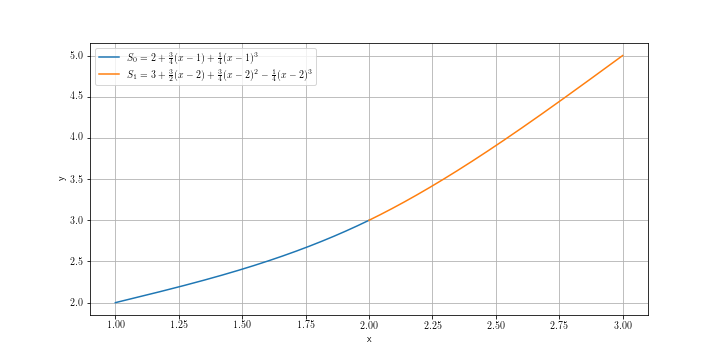
\includegraphics[width=14cm]{Images/ContohCubicSpline}
		\caption{Grafik dari Persamaan \eqref{SPContoh}}
	\end{figure}
	
\end{contoh}



\chapter{HERMITE KUBIK MONOTON}
Pada bab ini dibahas tentang dasar untuk membentuk interpolasi yang monoton, terutama interpolasi Hermite kubik monoton yang akan digunakan sebagai basis dalam pembentukan interpolasi spline kubik monoton.
\section{Interpolasi Monoton}

Untuk membentuk interpolasi monoton, perlu didefinisikan terlebih dulu sifat monoton fungsi.

\begin{definisi}\label{definisiMonoton}
     Misal $f:[a,b] \to \R$, dengan $f(a) \leq f(b)$ $(f(a) \geq f(b))$. Fungsi $f$ disebut \textbf{monoton naik (monoton turun)} pada interval $[a,b]$ jika untuk setiap $x,y \in [a,b]$ dengan $x \leq y$ berlaku
    \begin{equation*}
        f(x) \leq f(y),\:(f(x) \geq f(y)).
    \end{equation*}
\end{definisi}
\begin{contoh}
    Diberikan sebuah fungsi \(f:[0,1] \to \R\) dengan $f(x)=x^3$, untuk setiap $x \in [0,1]$. Fungsi $f$ merupakan fungsi monoton naik pada interval $[0,1]$ karena $f(0) = 0 \leq 1 = f(1)$ dan untuk setiap $x,y \in [0,1]$ dengan $x \leq y$ berlaku
    \begin{equation*}
        f(x) = x^2 \leq y^2 = f(y).
    \end{equation*}
\end{contoh}

Interpolasi adalah metode numerik yang menghasilkan titik baru diantara titik yang diberikan. Sebuah metode interpolasi dikatakan \textbf{monoton} jika hasil interpolasi memenuhi Definisi \ref{definisiMonoton} pada setiap interval tertutup diantara titik yang diberikan.

Sebuah interpolasi yang monoton memiliki banyak kelebihan, salah satunya hasil interpolasi lebih akurat untuk data yang diinterpolasi bersifat monoton. Sebagai contoh misalkan kita memiliki data $(0,10)$, $(1,8.7)$, $(2,2.1)$, $(3,1.5)$, dan $(4,0.1)$. Apabila diplot datanya akan diperoleh grafiknya sebagai berikut.
\begin{figure}[H]
    \centering
    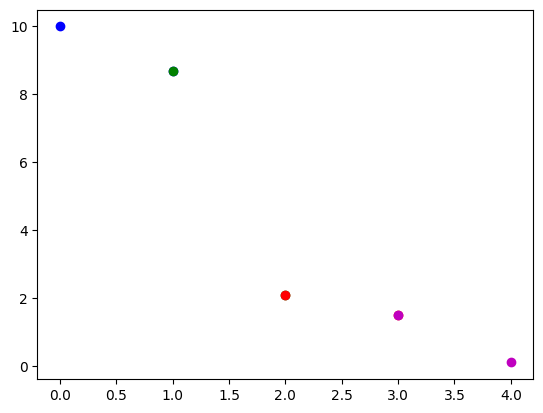
\includegraphics{Images/plotSplineKubik.png}
    \caption{Plot titik}
    \label{titik}
\end{figure}
Dari Gambar \ref{titik} dapat dilihat bahwa datanya monoton turun. Dalam menginterpolasi data tersebut, salah satu interpolasi yang dapat mempertahankan sifat monoton data adalah interpolasi linear. Dengan menggunakan metode interpolasi linear pada data, diperoleh grafik hasil interpolasinya berupa garis yang menghubungkan setiap titiknya.
\begin{figure}[H]
    \centering
    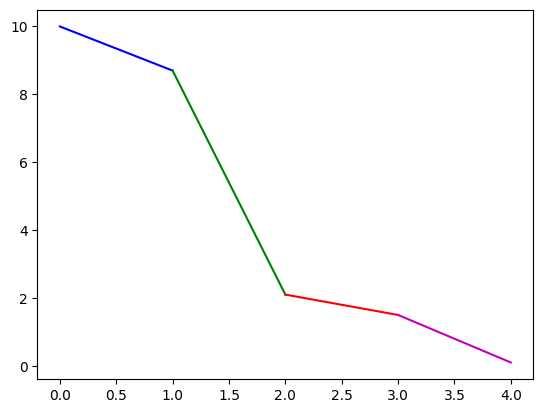
\includegraphics{Images/linear.png}
    \caption{Grafik interpolasi linear}
    \label{linear}
\end{figure}
Interpolasi linear pada Gambar \ref{linear} mempertahankan sifat monoton yang diinginkan tetapi hasil interpolasi yang diperoleh tidak dapat diturunkan pada titik-titik yang diinterpolasi.

Misalkan data yang diinterpolasikan pada Gambar \ref{titik} merupakan data kecepatan bola hingga berhenti dengan sumbu-$x$ berupa waktu dalam detik dan sumbu-$y$ berupa kecepatan bola dalam $m/s$. Jika perubahan kecepatan bola digambarkan menggunakan Gambar \ref{linear}, maka perubahan kecepatan bola pada titik data yang tidak mulus akan terjadi secara tidak wajar sehingga bola terlihat melambat secara tiba-tiba. Untuk menghindari hal tersebut data diinterpolasi menggunakan interpolasi spline kubik sehingga diperoleh grafik interpolasinya.
\begin{figure}[H]
    \centering
    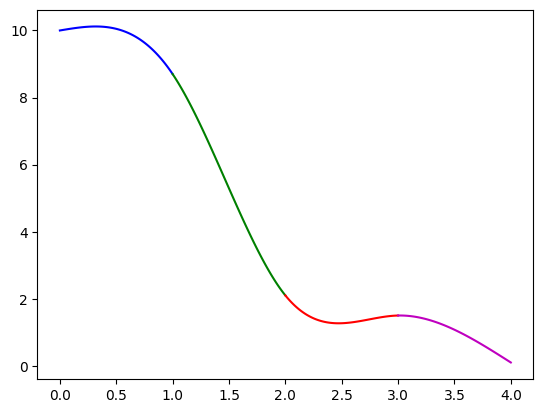
\includegraphics{Images/splineKubik.png}
    \caption{Grafik interpolasi spline kubik}
    \label{grafikHermite}
\end{figure}

Diperhatikan grafik interpolasi spline kubik pada Gambar \ref{grafikHermite} sudah terlihat mulus namun pada grafik tersebut data yang semula ingin dipertahankan sifat monotonnya menjadi hilang. Menghilangnya sifat monoton ini dapat menjadi masalah untuk nilai yang berada jauh dari nilai yang diinginkan. Seperti sebelumnya misal kita menginterpolasi data kecepatan bola tanpa menghiraukan arah bolanya, maka nilai kecepatan bola haruslah positif. Interpolasi yang tidak monoton menyebabkan nilai kecepatan bola berdasarkan hasil interpolasi dapat bernilai negatif. Hal ini menyebabkan hasil interpolasi tidak akurat.

\section{Interpolasi Hermite Kubik Monoton}
Pembentukan interpolasi spline kubik monoton diawali dengan pembentukan interpolasi Hermite kubik yang monoton. Polinomial hasil interpolasi Hermite kubik $P(x)$ pada titik-titik $x_1<\dots<x_n$ disebut monoton apabila untuk setiap $i=1,\:\dots,\:n-1$, polinomial kubik $P_i(x)$ pada interval $[x_i,x_{i+1}]$ yang didefinisikan seperti pada Persamaan \eqref{PersHermiteKubik} berupa
\begin{equation}\label{P_i}
    P_i(x)=f_i + \dot{f_i}(x-x_i) + \frac{(m_i-\dot{f_i})}{h_i}(x-x_i)^2 + \frac{(\dot{f_{i+1}}+\dot{f_i}-2m_i)}{h_i^2}(x-x_i)^2(x-x_{i+1}),
\end{equation}
merupakan polinomial yang monoton. 


Sebelum diberikan syarat interpolasi Hermite kubik dengan sifat monoton, akan diberikan terlebih dahulu syarat perlu Persamaan \eqref{P_i} hasil interpolasi Hermite kubik monoton pada interval $[x_i,x_{i+1}]$.

Berikut adalah syarat perlu agar Persamaan \eqref{P_i} monoton dengan
\begin{align*}
    sign(x) = \begin{cases}
        -1&, \quad x < 0, \\
        1&, \quad x > 0.
    \end{cases}
\end{align*}

\begin{teorema}\label{perluMonoton}
    Misal $P_i$ adalah polinomial hasil interpolasi Hermite kubik dari data $\{(x_i,f_i,\dot{f_i}),(x_{i+1},f_{i+1},\dot{f_{i+1}})\}$. Jika $P_i$ monoton pada $[x_i,x_{i+1}]$, maka 
    \begin{equation}
 sign(\dot{f_i})=sign(\dot{f_{i+1}})=sign(m_i).
    \end{equation}
    Lebih lanjut, jika $m_i=0$ maka $P_i$ konstan jika dan hanya jika $\dot{f_i}=\dot{f_{i+1}}=0$.
\end{teorema}
\begin{proof}
    Polinomial $P_i$ merupakan polinomial kubik pada interval $[x_i, x_{i+1}]$ yang monoton, sehingga diperoleh
    \begin{align*}
        \dot{f_i} = P_i'(x_i) &= \lim_{x \to x_i^+} \frac{P_i(x)-P_i(x_i)}{x-x_i}, \\
        \dot{f_{i+1}} = P_i'(x_{i+1}) &= \lim_{x \to x_{i+1}^-} \frac{P_i(x_{i+1})-P_i(x)}{x_{i+1}-x}, \\
        m_i = \frac{f(x_{i+1}) - f(x_i)}{x_{i+1}-x_i} &= \frac{P_i(x_{i+1}) - P_i(x_i)}{x_{i+1}-x_i}.
    \end{align*}
    Diperhatikan bahwa $P_i$ monoton, artinya $P_i(x) \leq P_i(y)$ atau $P_i(x) \geq P_i(y)$ untuk setiap $x,y \in [x_i,x_{i+1}]$ dengan $x \leq y$ sedemikian hingga diperoleh
    $$sign(\dot{f_i})=sign(\dot{f_{i+1}})=sign(m_i).$$

    Selanjutnya jika $m_i=0$ dan $P_i$ konstan, maka berdasarkan Persamaan \eqref{P_i} diperoleh
    \begin{align*}
        \dot{f_i} = 0, \\
        m_i-\dot{f_i} = 0, \\
        \dot{f_{i+1}}+\dot{f_i}-2m_i = 0,
    \end{align*}
    sehingga diperoleh $\dot{f_i}=\dot{f_{i+1}}=0$.

    Sebaliknya jika $m_i=\dot{f_i}=\dot{f_{i+1}}=0$ maka polinomial pada Persamaan \eqref{P_i} berbentuk
    \begin{equation*}
        P_i(x)=f_i,
    \end{equation*}
    sehingga diperoleh $P_i$ konstan.
\end{proof}

Setelah diberikan syarat perlu Persamaan \eqref{P_i} monoton pada Teorema \ref{perluMonoton}, selanjutnya akan diselidiki syarat cukup agar polinomialnya monoton. Interpolasi Hermite kubik memiliki polinomial $P_i(x)$ untuk $x \in [x_i,x_i+1]$ yang diperoleh pada Persamaan \eqref{P_i} memilki deret Taylor di titik $x=x_i$ berupa
\begin{equation}\label{taylorHermite}
\begin{split}
    P_i(x) &= P_i(x_i) + P_i'(x_i)(x-x_i) + \frac{P_i''(x_i)}{2}(x-x_i)^2 + \frac{P_i'''(x_i)}{6}(x-x_i)^3 \\
    &= f_i + \dot{f_i}(x-x_i) + \frac{(-2\dot{f_i}-\dot{f_{i+1}}+3m_i)}{h_i}(x-x_i)^2 + \frac{(\dot{f_i}+\dot{f_{i+1}}-2m_i)}{h_i^2}(x-x_i)^3,
\end{split}
\end{equation}
sehingga diperoleh
\begin{equation}\label{taylorHermite2}
    P_i'(x) = \dot{f_i} + \frac{2(-2\dot{f_i}-\dot{f_{i+1}}+3m_i)}{h_i}(x-x_i) + \frac{3(\dot{f_i}+\dot{f_{i+1}}-2m_i)}{h_i^2}(x-x_i)^2,
\end{equation}
dan
\begin{equation}
    P_i''(x) = \frac{2(-2\dot{f_i}-\dot{f_{i+1}}+3m_i)}{h_i} + \frac{6(\dot{f_i}+\dot{f_{i+1}}-2m_i)}{h_i^2}(x-x_i).
\end{equation}

Berdasarkan ketunggalan polinomial Hermite, polinomial $P_i$ yang diperoleh dari deret Taylornya adalah polinomial yang sama dengan polinomial Hermite pada Persamaan \eqref{P_i}. Untuk memudahkan penulisan selanjutnya akan definisikan \mbox{$\alpha_i := \dot{f_i}/m_i$} dan $\beta_i := \dot{f_{i+1}}/m_i$.
\begin{lemma}\label{lema1}
     Misal $P_i$ adalah polinomial hasil interpolasi Hermite kubik dari data $\{(x_i,f_i,\dot{f_i}),(x_{i+1},f_{i+1},\dot{f_{i+1}})\}$. Jika $\alpha_i + \beta_i - 2 \leq 0$, maka polinomial $P_i$ monoton pada $[x_i,x_{i+1}]$ jika dan hanya jika syarat perlu monoton pada Teorema \ref{perluMonoton} terpenuhi.
\end{lemma}

\begin{proof}    
Dengan asumsi bahwa $m_i \neq 0$ dan syarat perlu monoton pada Teorema \ref{perluMonoton} terpenuhi, ditinjau dua kasus di mana $\alpha_i + \beta_i - 2 = 0$ dan $\alpha_i + \beta_i - 2 < 0$.

Untuk kasus pertama ketika $\alpha_i + \beta_i - 2 = 0$, diperhatikan bahwa 
$$\alpha_i + \beta_i - 2 = \frac{\dot{f_{i+1}}+\dot{f_i}-2m_i}{m_i},$$ sehingga diperoleh $\dot{f_{i+1}}+\dot{f_i}-2m_i = 0$. Hal ini mengakibatkan polinomial $P_i(x)$ merupakan polinomial berderajat dua berdasarkan Persamaan \eqref{taylorHermite} dan $P_i'$ linear atau konstan. Polinomial $P_i'$ linear atau konstan sehingga pada interval $[x_{i},x_{i+1}]$ grafiknya berupa garis lurus. Hal ini berakibat pada $P_i'$ berlaku 
\begin{align*}
    \min(\dot{f_i},\dot{f_{i+1}}) \leq P_i'(x) \leq \max(\dot{f_i},\dot{f_{i+1}}),
\end{align*} 
untuk setiap $x \in [x_i,x_{i+1}]$. Lalu dikarenakan syarat perlu monoton pada Teorema \ref{perluMonoton} terpenuhi, maka dapat disimpulkan $P_i'(x)$ tidak berganti tanda pada interval $[x_i,x_{i+1}]$ berakibat $P_i$ monoton.

Untuk kasus kedua ketika $\alpha_i + \beta_i - 2 < 0$, diperhatikan bahwa  $$\alpha_i + \beta_i - 2 = \frac{\dot{f_{i+1}}+\dot{f_i}-2m_i}{m_i},$$ sehingga diperoleh $\dot{f_{i+1}}+\dot{f_i}-2m_i \neq 0$. Hal ini mengakibatkan polinomial $P_i$ merupakan polinomial berderajat tiga sehingga diperoleh $P_i'(x)$ merupakan polinomial berderajat dua.

Diperhatikan jika $\dot{f_{i+1}}+\dot{f_i}-2m_i > 0$ maka $P_i'(x)$ merupakan kurva cekung ke atas sedangkan jika $\dot{f_{i+1}}+\dot{f_i}-2m_i < 0$ maka $P_i'(x)$ merupakan kurva cekung ke bawah. Jika $f_i < f_{i+1}$ berakibat $m_i > 0$ dan $P_i'(x)$ cekung ke bawah, maka $P_i(x)$ merupakan fungsi yang monoton naik dikarenakan $0 \leq \min(\dot{f_i},\dot{f_{i+1}}) \leq P_i'(x)$ untuk setiap $x \in [x_i,x_{i+1}]$. Sebaliknya juga berlaku yaitu jika $f_i > f_{i+1}$ berakibat $m_i < 0$ dan $P_i'(x)$ cekung ke atas, maka $P_i(x)$ merupakan fungsi yang monoton turun dikarenakan $P_i'(x) \leq \max(\dot{f_i},\dot{f_{i+1}}) \leq 0$ untuk setiap $x \in [x_i,x_{i+1}]$.
\end{proof}

\begin{contoh}
    Diberikan set data $\{(1,2,2),(3,6,1)\}$, diperoleh $m_i=2$, $\alpha_i=1$ dan $\beta_i=0.5$. Dari situ diperoleh $\alpha_i+\beta_i-2=-0.5\leq0$ yang berdasarkan Lema \ref{lema1} hasil interpolasi Hermite kubiknya monoton.
    \begin{figure}[H]
        \centering
        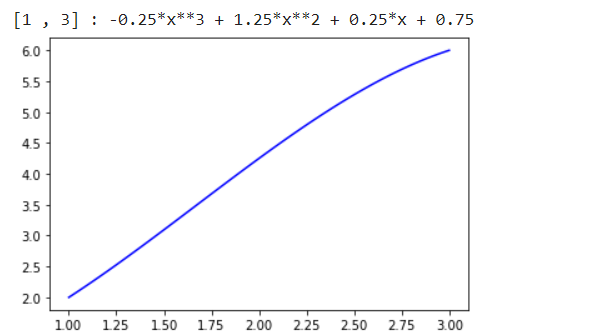
\includegraphics[width=10cm]{Images/contohLema1Hermite.png}
        \caption{Hasil interpolasi Hermite kubik $\{(1,2,2),(3,6,1)\}$ menggunakan \textit{Python}}
        \label{Gambar3.4}
    \end{figure}
    Interpolasi dicari dengan menggunakan bahasa pemrograman \textit{Python}. Dalam hal ini, diperoleh grafik hasil interpolasinya yaitu Gambar \ref{Gambar3.4}. Diperhatikan bahwa hasil grafik interpolasi Hermite kubik yang diperoleh monoton sesuai dengan Lema \ref{lema1}.
\end{contoh}

Setelah sebelumnya ditinjau syarat cukup polinomial Hermite kubik $P_i$ monoton ketika $(\alpha_i + \beta_i - 2) \leq 0$, selanjutnya akan ditinjau syarat cukup polinomial Hermite kubik $P_i$ monoton ketika $(\alpha_i + \beta_i - 2) > 0$.

\begin{lemma}\label{lema2}
    Jika  $(\alpha_i + \beta_i - 2) > 0$ dan syarat perlu monoton pada Teorema \ref{perluMonoton} terpenuhi, maka polinomial Hermite kubik $P_i(x)$ monoton pada $[x_i,x_{i+1}]$ jika dan hanya jika salah satu dari kondisi berikut terpenuhi
    \begin{enumerate}
        \item $2\alpha_i+\beta_i-3 \leq 0$,
        \item $\alpha_i+2\beta_i-3 \leq 0$,
        \item $\phi(\alpha_i, \beta_i) > 0$, dengan $ \phi(\alpha,\beta) = \alpha - \frac{1}{3}\frac{(2\alpha + \beta -3)^2}{\alpha + \beta - 2}$.
    \end{enumerate}
\end{lemma}
\begin{proof}
Ketika $(\alpha_i + \beta_i - 2) > 0$. Diperhatikan bahwa $\alpha_i$ dan $\beta_i$ selalu bernilai nonnegatif ketika syarat perlu monoton pada Teorema \ref{perluMonoton} terpenuhi. $P_i'(x)$ berdasarkan Persamaan \eqref{taylorHermite2} mempunyai titik ekstremum di
\begin{equation}\label{3.6}
    x^\star = x_i + \frac{h_i}{3}[\frac{2\alpha_i + \beta_i - 3}{\alpha_i + \beta_i - 2}],
\end{equation}
dan
\begin{equation}
    P_i'(x^\star) = \phi(\alpha_i,\beta_i)m_i,
\end{equation}
dengan
\begin{equation}\label{3.7}
    \phi(\alpha,\beta) = \alpha - \frac{1}{3}\frac{(2\alpha + \beta -3)^2}{\alpha + \beta - 2}.
\end{equation}
$P_i(x)$ monoton jika dan hanya jika salah satu dari kondisi berikut terpenuhi
\begin{enumerate}
    \item $x^\star \notin [x_i,x_{i+1}]$,
    \item $x^\star \in [x_i,x_{i+1}]$ dan $sign(P_i'(x^\star))=sign(m_i)$.
\end{enumerate}

Diperoleh dari Persamaan \eqref{3.6} kondisi pertama dapat dituliskan sebagai $x^\star > x_{i+1}$ atau $x^\star < x_{i}$ yang apabila dijabarkan diperoleh
        \begin{align*}
             &&x^\star < x_i \\
             &\Rightarrow&x_i + \frac{h_i}{3}[\frac{2\alpha_i + \beta_i - 3}{\alpha_i + \beta_i - 2}] < x_i,\\
             &\Rightarrow&\frac{h_i}{3}[\frac{2\alpha_i + \beta_i - 3}{\alpha_i + \beta_i - 2}] < 0,\\
             &\Rightarrow&2\alpha_i+\beta_i-3 < 0,
        \end{align*}
dan
\begin{align*}
             &&x^\star > x_i \\
             &\Rightarrow&x_i + \frac{h_i}{3}[\frac{2\alpha_i + \beta_i - 3}{\alpha_i + \beta_i - 2}] > x_i + h_i,\\
             &\Rightarrow&\frac{h_i}{3}[\frac{2\alpha_i + \beta_i - 3}{\alpha_i + \beta_i - 2}] > h_i,\\
             &\Rightarrow&2\alpha_i + \beta_i - 3 > 3\alpha_i+3\beta_i-6,\\
             &\Rightarrow&\alpha_i+2\beta_i-3 < 0.
        \end{align*} 
Sedangkan untuk kondisi kedua dari Persamaan \eqref{3.7} dapat diartikan bahwa $$\phi(\alpha_i, \beta_i) > 0,$$
\end{proof}
sehingga diperoleh
\begin{align*}
    &&\phi(\alpha_i, \beta_i) > 0, \\
    &\Rightarrow&\alpha_i - \frac{1}{3}\frac{(2\alpha_i + \beta_i -3)^2}{\alpha_i + \beta_i - 2}>0, \\
    &\Rightarrow&-\alpha_i(3(\alpha_i + \beta_i -2)) + (2\alpha_i + \beta_i - 3)^2 < 0, \\
    &\Rightarrow&-3\alpha_i^2 - 3 \alpha_i\beta_i + 6 \alpha_i + 4\alpha_i^2 + 4\alpha_i\beta_i - 12\alpha_i + \beta_i^2 - 6\beta_i + 9 < 0, \\
    &\Rightarrow&\alpha_i^2 + \beta_i^2 + \alpha_i\beta_i - 6\alpha_i -6\beta_i + 9 < 0, \\
    &\Rightarrow&\alpha_i^2 + \alpha_i(\beta_i - 6) + (\beta_i - 3)^2 < 0,
\end{align*}
yang merupakan daerah didalam elips dengan pusat $(2,2)$. 
\begin{figure}[H]
    \centering
    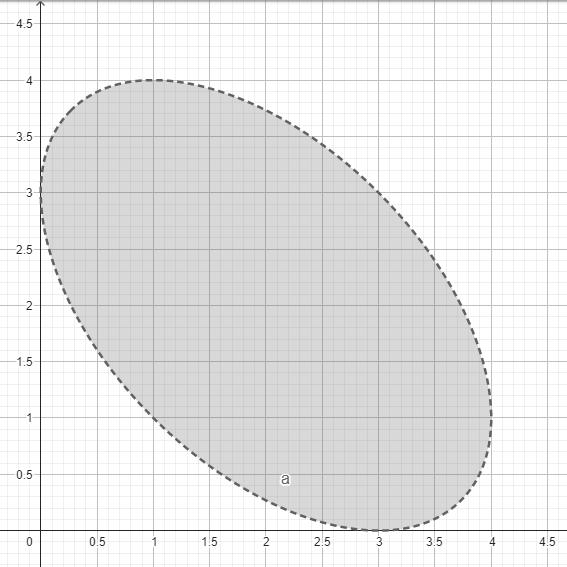
\includegraphics[width=10cm]{Images/daerahMonotonElips.png}
    \caption{Daerah elips $\alpha_i^2 + \alpha_i(\beta_i - 6) + (\beta_i - 3)^2 < 0$, dengan sumbux-$x$ adalah $\alpha$ dan sumbu-$y$ adalah $\beta$}
    \label{fig:my_label}
\end{figure}


\begin{contoh}
     Diberikan set data $\{(1,2,1),(2,4,4)\}$ sehingga $m_i=2$, $\alpha_i=0.5$ dan $\beta_i=2$. Dari situ diperoleh $\alpha_i+\beta_i-2=0.5>0$ dan $2\alpha_i+\beta_i-3 = 0 $ yang berdasarkan Lema \ref{lema2} hasil interpolasi Hermite kubiknya monoton.
     \begin{figure}[H]
         \centering
         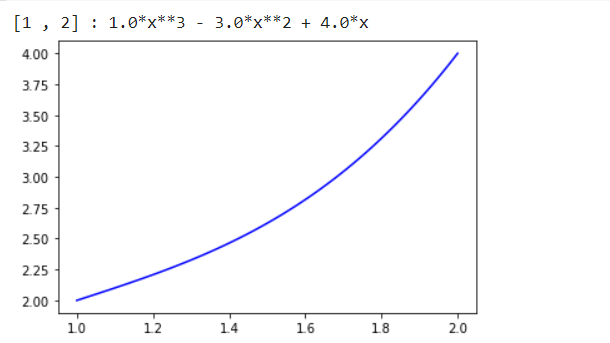
\includegraphics[width=10cm]{Images/contohLema2.1Hermite.png}
         \caption{Hasil interpolasi Hermite kubik $\{(1,2,1),(2,4,4)\}$ menggunakan \textit{Python}}
         \label{Gambar3.6}
     \end{figure}
     Untuk kondisi kedua dipilih set data $\{(1,2,4),(2,4,1)\}$ sehingga $m_i=2$, $\alpha_i=2$ dan $\beta_i=0.5$. Dari situ diperoleh $\alpha_i+\beta_i-2=0.5>0$ dan \mbox{$\alpha_i+2\beta_i-3 = 0 $} sehingga berdasarkan Lema \ref{lema2} dapat disimpulkan hasil interpolasi Hermite kubiknya monoton.
     \begin{figure}[H]
         \centering
         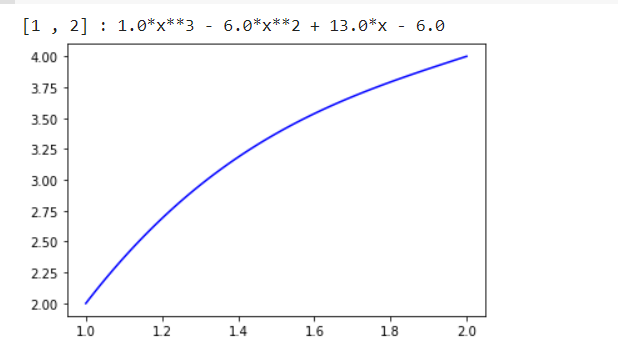
\includegraphics[width=10cm]{Images/contohLema2.2Hermite.png}
         \caption{Hasil interpolasi Hermite kubik $\{(1,2,4),(2,4,1)\}$ menggunakan \textit{Python}}
         \label{Gambar3.7}
     \end{figure}
     Terakhir, untuk kondisi ketiga dipilih set data $\{(1,2,4),(2,4,2)\}$ sehingga $m_i=2$, $\alpha_i=2$ dan $\beta_i=1$. Dari situ diperoleh $\alpha_i+\beta_i-2=1>0$ dan 
     $$\phi(\alpha_i,\beta_i) = 2 - \frac{1}{3}\frac{(2)^2}{1}=\frac{8}{3}>0,$$ sehingga interpolasi Hermite kubiknya yang dihasilkan monoton.
     \begin{figure}[H]
         \centering
         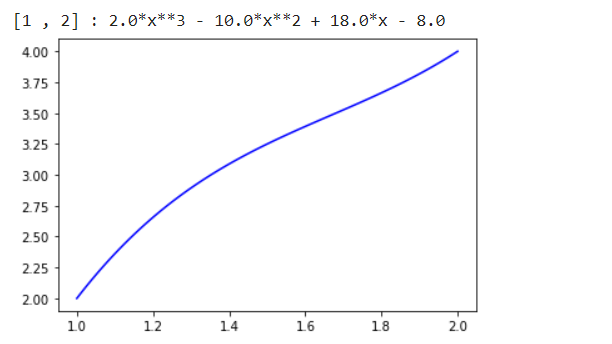
\includegraphics[width=10cm]{Images/contohLema2.3Hermite.png}
         \caption{Hasil interpolasi Hermite kubik $\{(1,2,4),(2,4,2)\}$ menggunakan \textit{Python}}
         \label{Gambar3.8}
     \end{figure}

     Pada ketiga contoh yang diberikan, diperoleh hasil interpolasi monoton pada Gambar \ref{Gambar3.6}, Gambar \ref{Gambar3.7}, dan Gambar \ref{Gambar3.8}. Hal ini sesuai dengan yang diberikan pada Lema \ref{lema2}.
\end{contoh}

Dari kedua lema yang baru saja diberikan dapat dibentuk daerah monoton berdasarkan nilai $\alpha_i$ dan $\beta_i$.

\begin{figure}[H]
    \centering
    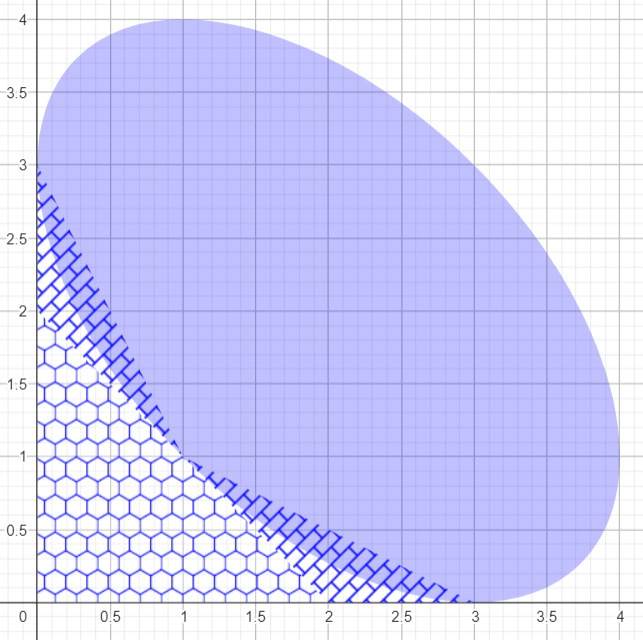
\includegraphics[width=10cm]{Images/Daerah monoton}
    \caption{Daerah Monoton Berdasarkan $\alpha_i$ dan $\beta_i$, dengan sumbux-$x$ adalah $\alpha$ dan sumbu-$y$ adalah $\beta$}
    \label{daerahmonoton}
\end{figure}

Kondisi untuk $\alpha_i$ dan $\beta_i$ yang diperoleh pada Lema \ref{lema1} dan Lema \ref{lema2} dapat digambarkan sebagai daerah arsiran pada Gambar \ref{daerahmonoton} dengan sumbu absis merupakan $\alpha_i$ dan sumbu ordinat merupakan $\beta_i$. Daerah yang diarsir merupakan daerah saat fungsi $P_i(x)$ monoton sesuai dengan Lema \ref{lema1} dan Lema \ref{lema2}.

\begin{teorema}\label{ab_leq3}
    Misal $I_i = [x_i,x_{i+1}]$ dan $P_i$ adalah polinomial hasil interpolasi Hermite kubik dari data $\{(x_i,f_i,\dot{f_i}),(x_{i+1},f_{i+1},\dot{f_{i+1}})\}$.
    Jika
    \begin{equation*}
        0 \leq \alpha_i, \beta_i \leq 3,
    \end{equation*}
    maka polinomial $P_i$ monoton pada $I_i$.
\end{teorema}

\begin{proof}
    Diperhatikan pada Gambar \ref{daerahmonoton} yang dibuat berdasarkan hasil Lema \ref{lema1} dan Lema \ref{lema2}, $0 \leq \alpha_i, \beta_i \leq 3$ berada pada daerah arsiran sehingga polinomial $P_i$ monoton pada $I_i$.
\end{proof}

\begin{teorema}\label{3.1.7}
    Misal $I_i = [x_i,x_{i+1}]$ dan $P_i$ adalah polinomial Hermite kubik yang menginterpolasi data $\{(x_i,f_i,\dot{f_i}),(x_{i+1},f_{i+1},\dot{f_{i+1}})\}$.
    Jika syarat perlu monoton
    \begin{align*}
     sign(\dot{f_i})=sign(\dot{f_{i+1}})=sign(m_i),
    \end{align*}
    untuk setiap $i=1,\dots,n-1$ terpenuhi dan
    \begin{equation*}
        |\dot{f_i}| \leq 3 \min(|m_{i-1}|,|m_i|)
    \end{equation*}
    untuk setiap $i=2,\dots,n-1$, maka polinomial $P_i$ monoton pada semua interval $I_i$, $i=1,\:2,\dots,\:n-1$.
\end{teorema}

\begin{proof}
    Diketahui untuk setiap $i=1,\:2,\dots,\:n-1$
    \begin{align*}
     sign(\dot{f_i})=sign(\dot{f_{i+1}})=sign(m_i),
    \end{align*}
    dan
    \begin{equation*}
        |\dot{f_i}| \leq 3 \min(|m_{i-1}|,|m_i|),
    \end{equation*}
    akibatnya diperoleh
    \begin{equation*}
        0 \leq \frac{\dot{f_i}}{m_i} \leq 3,
    \end{equation*}
    dan
    \begin{equation*}
        0 \leq \frac{\dot{f_{i+1}}}{m_i} \leq 3,
    \end{equation*}
    sedemikian hingga berlaku untuk setiap $i=1,\:2,\dots,\:n-2$
    \begin{equation*}
        0 \leq \alpha_i, \beta_i \leq 3.
    \end{equation*}
    Berdasarkan Teorema \ref{ab_leq3} diperoleh $P_i$ monoton pada setiap interval $I_i$ untuk setiap $i=1,\:2,\dots,\:n-2$.
\end{proof}

\begin{teorema}
    Misal $I_i = [x_i,x_{i+1}]$ dan $P_i$ adalah polinomial Hermite kubik yang menginterpolasi data $\{(x_i,f_i,\dot{f_i}),(x_{i+1},f_{i+1},\dot{f_{i+1}})\}$.
    Jika salah satu dari kondisi berikut terpenuhi
    \begin{enumerate}
        \item $0 \leq \alpha_i + \beta_i \leq 3$,
        \item $\alpha_i^2 + \alpha_i(\beta_i-6) + (\beta_i-3)^2 < 0,$
    \end{enumerate}
    $\forall i = 0, \dots, n-1$ maka polinomial $P_i$ monoton pada $I_i$.
\end{teorema}

\begin{proof}
Diperhatikan bahwa kondisi pertama merupakan daerah di dalam arsiran pada Gambar \ref{daerahmonoton} sehingga $P_i$ monoton pada $[x_i, x_{i+1}]$.
Untuk kondisi kedua berdasarkan Lema \ref{lema2} yaitu jika $\phi(\alpha_i, \beta_i) > 0$, dengan
\begin{equation}
    \phi(\alpha,\beta) = \alpha - \frac{1}{3}\frac{(2\alpha + \beta -3)^2}{\alpha + \beta - 2}
\end{equation}
maka polinomial Hermite kubik $P_i$ yang menginterpolasi data $\{(x_i,f_i,\dot{f_i}),(x_{i+1},f_{i+1},\dot{f_{i+1}})\}$ monoton pada interval $[x_i, x_{i+1}]$. Diperoleh,
\begin{align*}
    &&\phi(\alpha_i, \beta_i) > 0, \\
    &\Rightarrow&\alpha_i - \frac{1}{3}\frac{(2\alpha_i + \beta_i -3)^2}{\alpha_i + \beta_i - 2}>0, \\
    &\Rightarrow&-\alpha_i(3(\alpha_i + \beta_i -2)) + (2\alpha_i + \beta_i - 3)^2 < 0, \\
    &\Rightarrow&-3\alpha_i^2 - 3 \alpha_i\beta_i + 6 \alpha_i + 4\alpha_i^2 + 4\alpha_i\beta_i - 12\alpha_i + \beta_i^2 - 6\beta_i + 9 < 0, \\
    &\Rightarrow&\alpha_i^2 + \beta_i^2 + \alpha_i\beta_i - 6\alpha_i -6\beta_i + 9 < 0, \\
    &\Rightarrow&\alpha_i^2 + \alpha_i(\beta_i - 6) + (\beta_i - 3)^2 < 0,
\end{align*}

 Dapat disimpulkan bahwa jika kondisi kedua terpenuhi, maka $P_i$ monoton pada $[x_i, x_{i+1}]$.
\end{proof}
\begin{lemma}\label{orderAkurasi}
    Misal $f(x)$ fungsi yang mulus. Jika $\dot{f_i}=f'(x_i) + O(h^{q_i})$ dan $\dot{f_{i+1}}=f'(x_{i+1}) + O(h^{q_{i+1}})$, maka polinomial interpolasi Hermite kubik sepotong-sepotong pada interval $[x_i,x_{i+1}]$ memenuhi,
    \begin{equation*}
        P_i(x) = f(x) + O(h^q)
    \end{equation*}
    dengan $q=\min(4, q_i+1, q_{i+1}+1)$.
\end{lemma}

\begin{proof}
    Pertama-tama diambil dari Persamaan \eqref{errorHermiteKubik} diperoleh polinomial interpolasi $P_i$ memiliki order akurasi $O(h^4)$ untuk $\dot{f_i}=f'(x_i)$ dan $\dot{f_{i+1}}=f'(x_{i+1})$ sehingga
    \begin{align*}
        f(x) = P_i(x) + O(h^4).
    \end{align*}
    Diperhatikan apabila disubtitusikan $\dot{f_i}=f'(x_i) + O(h^{q_i})$ dan \mbox{$\dot{f_{i+1}}=f'(x_{i+1}) + O(h^{q_{i+1}})$} pada polinomial interpolasi Hermite kubik seperti pada Persamaan \eqref{PersHermiteKubik}, maka diperoleh
    \begin{align*}
        f(x) =& f_i + (f'(x_i) + O(h^{q_i}))(x-x_i) + \frac{(m_i-(f'(x_i) + O(h^{q_i}))}{h_i}(x-x_i)^2 \\
        &+ \frac{((f'(x_{i+1}) + O(h^{q_{i+1}}))+(f'(x_i) + O(h^{q_i}))-2m_i)}{h_i^2}(x-x_i)^2(x-x_{i+1}) + O(h^4) \\
        =& P_i(x) + O(h^{q_i})(x-x_i) + \frac{O(h^{q_i})}{h_i}(x-x_i)^2 \\
        &+ \frac{(O(h^{q_i}) + O(h^{q_{i+1}}))}{h_i^2}(x-x_i)^2(x-x_{i+1}) + O(h^{4}),
    \end{align*}
    yang berakibat
    \begin{gather*}
        f(x)\leq P_i(x) + O(h^{q_i+1}) + O(h^{q_i+1}) + O(h^{\min(q_i+1,q_{i+1}+1)}) + O(h^{4}),
    \end{gather*}
    sehingga dapat disimpulkan
    \begin{equation*}
        P_i(x) = f(x) + O(h^q),
    \end{equation*}
    dengan $q=\min(4, q_i+1, q_{i+1}+1)$.
\end{proof}

\begin{contoh}
Dipilih fungsi $f(x) = \sin(x)$ pada interval $[0,1]$. Interval tersebut dibagi menjadi beberapa subinterval. Jika $\dot{f} = f'(x)=\cos(x)$, maka akan ditinjau hasil galat dari interpolasi Hermite kubik pada titik $x=0,3$ yang memiliki order akurasi $O(h^4)$ sehingga dengan simulasi menggunakan bahasa pemrograman \textit{Python} diperoleh hasil galat dari interpolasinya.

\begin{table}[htp]
        \centering
        \begin{tabular}{|c|c|c|c|c|c|}
    \hline $h$& galat di $x = 0.3$ \\ 
    \hline
0.5&$3.84021 \times 10^{-5}$  \\
0.25&$1.46615 \times 10^{-6}$ \\
0.125&$1.78698 \times 10^{-7}$  \\
0.0625&$4.57581 \times 10^{-9}$  \\
    \hline
    \end{tabular}
        \caption{Interpolasi Hermite kubik dari fungsi $f(x)=\sin(x)$ di titik $x=0.3$, dengan turunan analitik}
        \label{contohOrderAkurasi1}
\end{table}
    
Selanjutnya, akan dibandingkan apabila nilai dari $\dot{f}$ merupakan hasil pendekatan dengan menggunakan metode beda bagi tengah yang memiliki order akurasi $O(h^2)$ sehingga hasil polinomial interpolasi yang diperoleh memiliki order akurasi $O(h^3)$ berdasarkan Lema \ref{orderAkurasi}.
\begin{table}[htp]
        \centering
        \begin{tabular}{|c|c|c|c|c|c|}
    \hline $h$& galat di $x = 0.3$ \\ 
    \hline
0.5&$0.00256163$  \\
0.25&$0.000250525 $ \\
0.125&$1.65053 \times 10^{-5}$  \\
0.0625&$3.68918 \times 10^{-6}$  \\
    \hline
    \end{tabular}
        \caption{Interpolasi Hermite kubik dari fungsi $f(x)=\sin(x)$ di titik $x=0.3$, dengan menggunakan metode beda bagi tengah}
        \label{contohOrderAkurasi2}
\end{table}
Terakhir akan ditinjau ketika nilai $\dot{f}$ dicari dengan menggunakan metode beda bagi maju yang mempunyai order akurasi $O(h)$ sehingga polinomial interpolasi yang dihasilkan memiliki order akurasi $O(h^2)$.

\begin{table}[htp]
        \centering
        \begin{tabular}{|c|c|c|c|c|c|}
    \hline $h$& galat di $x = 0.3$  \\ 
    \hline
0.5&$0.011013$  \\
0.25&$0.000758064 $ \\
0.125&$2.01257 \times 10^{-5}$  \\
0.0625&$6.50661 \times 10^{-5}$  \\
    \hline
    \end{tabular}
        \caption{Interpolasi Hermite kubik dari fungsi $f(x)=\sin(x)$ di titik $x=0.3$, dengan menggunakan metode beda bagi maju}
        \label{contohOrderAkurasi3}
\end{table}
Diperhatikan bahwa, Tabel \ref{contohOrderAkurasi1} memiliki galat yang paling kecil dibandingkan dua tabel lain yang diberikan. Tabel \ref{contohOrderAkurasi3} memiliki galat yang paling besar dibandingkan dua tabel lainnya. Hal ini sesuai dengan yang diberikan pada Lema \ref{orderAkurasi}.
\end{contoh}


\chapter{SPLINE KUBIK MONOTON}
Pada bab ini akan disampaikan hal-hal berkaitan dengan pembuatan interpolasi spline kubik yang monoton. 

\section{Interpolasi Spline Kubik Monoton}

Setelah diperoleh syarat-syarat cukup sebuah polinomial interpolasi Hermite kubik monoton pada suatu interval selanjutnya akan dibentuk polinomial spline kubik $P_i(x)$ yang memenuhi kondisi
\begin{align}
    P_i^{(k)}(x_{i+1}) = P_{i+1}^{(k)}(x_{i+1}), \: k=0,1,2,\label{3.10} \\
    P_1'(x_1) = \dot{f_1} := f'(x_1) = f_1', \label{3.11} \\
    P_{n-1}'(x_n) = \dot{f_n} := f'(x_n) = f_n' \label{3.12}
\end{align}
dengan $i=1,~2,\dots,~n-2$.

Diperhatikan polinomial Hermite kubik yang telah diperoleh sebelumnya telah memenuhi kondisi Persamaan \eqref{3.10}, \eqref{3.11}, dan \eqref{3.12} untuk $k=0,1$. Selanjutnya polinomial Hermite kubik pada Persamaan \eqref{P_i} tersebut akan digunakan untuk memperoleh polinomial yang memenuhi kondisi Persamaan \eqref{3.10} untuk kasus $k=2$.

Dari Persamaan \eqref{P_i} yang merupakan polinomial Hermite kubik $P_i(x)$ untuk $x \in [x_i,x_{i+1}]$, diperoleh $P_i''(x)$ sebagai berikut
\begin{equation}
    P_i''(x) = \frac{2(m_i-\dot{f_i})}{h_i} + \frac{4(\dot{f_{i+1}}+\dot{f_i}-2m_i)}{h_i^2}(x-x_i) +\frac{2(\dot{f_{i+1}}+\dot{f_i}-2m_i)}{h_i^2}(x-x_{i+1}),
\end{equation}
sedemikian hingga
\begin{align*}
    P_i''(x_{i+1}) &= \frac{2(m_i-\dot{f_i})}{h_i} + \frac{4(\dot{f_{i+1}}+\dot{f_i}-2m_i)}{h_i^2}(x_{i+1}-x_i) \\
    &+\frac{2(\dot{f_{i+1}}+\dot{f_i}-2m_i)}{h_i^2}(x_{i+1}-x_{i+1})\\
    &=\frac{2(m_i-\dot{f_i})}{h_i}+\frac{4(\dot{f_{i+1}}+\dot{f_i}-2m_i)}{h_i^2}h_i\\
    &=2\frac{\dot{f_i}}{h_i} + 4\frac{\dot{f_{i+1}}}{h_i} - 6\frac{m_i}{h_i},
\end{align*}
dan
\begin{align*}
    P_{i+1}''(x_{i+1}) &= \frac{2(m_{i+1}-\dot{f_{i+1}})}{h_{i+1}} + \frac{4(\dot{f_{i+2}}+\dot{f_{i+1}}-2m_{i+1})}{h_{i+1}^2}(x_{i+1}-x_{i+1}) \\
    &+\frac{2(\dot{f_{i+2}}+\dot{f_{i+1}}-2m_{i+1})}{h_{i+1}^2}(x_{i+1}-x_{i+2})\\
    &=\frac{2(m_{i+1}-\dot{f_{i+1}})}{h_{i+1}}+\frac{2(\dot{f_{i+2}}+\dot{f_{i+1}}-2m_{i+1})}{h_{i+1}^2}h_{i+1}\\
    &=-4\frac{\dot{f_{i+1}}}{h_{i+1}} - 2\frac{\dot{f_{i+2}}}{h_{i+1}} + 6\frac{m_{i+1}}{h_{i+1}}.
\end{align*}

Berdasarkan Persamaan \eqref{3.10} untuk kasus $k=2$ diperoleh
\begin{align*}
        &&P_i''(x_{i+1}) &= P_{i+1}''(x_{i+1}), \\
        &\Rightarrow& 
        2\frac{\dot{f_i}}{h_i} + 4\frac{\dot{f_{i+1}}}{h_i} - 6\frac{m_i}{h_i} &= -4\frac{\dot{f_{i+1}}}{h_{i+1}} - 2\frac{\dot{f_{i+2}}}{h_{i+1}} + 6\frac{m_{i+1}}{h_{i+1}}, \\
        &\Rightarrow&
        \frac{\dot{f_i}}{h_i} + 2\left( \frac{1}{h_i} + \frac{1}{h_{i+1}} \right)\dot{f_{i+1}} + \frac{\dot{f_{i+2}}}{h_{i+1}} &= 3\left( \frac{m_i}{h_i} + \frac{m_{i+1}}{h_{i+1}} \right),\\
        &\Rightarrow&\frac{h_{i+1}}{h_i + h_{i+1}}\dot{f_i} + 2\dot{f_{i+1}} + \frac{h_i}{h_i + h_{i+1}}\dot{f_{i+2}} &= 3\left( \frac{h_{i+1}}{h_i + h_{i+1}}m_i + \frac{h_i}{h_i + h_{i+1}}m_{i+1} \right).
        % \frac{h_ih_{i+1}}{h_i + h_{i+1}}&
\end{align*}
Selanjutnya apabila ditambahkan kondisi pada Persamaan \eqref{3.11} dan \eqref{3.12} dengan $\dot{f_1} = f_1'$ dan $\dot{f_n} = f_n'$ diperoleh
\begin{align*}
2\dot{f_{2}} + \frac{h_1}{h_1 + h_{2}}\dot{f_{3}} = 3\left( \frac{h_{2}}{h_1 + h_{2}}m_1 + \frac{h_1}{h_1 + h_{2}}m_{2} \right) - \frac{h_{2}}{h_1 + h_{2}}f_1',
\end{align*}
dan
\begin{align*}
\frac{h_{n-1}}{h_{n-2} + h_{n-1}}\dot{f_{n-2}} + 2\dot{f_{n-1}} = 3\left( \frac{h_{n-1}}{h_{n-2} + h_{n-1}}m_{n-2} + \frac{h_{n-2}}{h_{n-2} + h_{n-1}}m_{n-1} \right) - \frac{h_{n-2}}{h_{n-2} + h_{n-1}}f_{n}',
\end{align*}
sedemikian hingga diperoleh sistem persamaan
\begin{gather}\label{3.14}
    \begin{split}
    2\dot{f_2} + \mu_1\dot{f_3} &= b_2, \\
    \lambda_i\dot{f_i} + 2\dot{f_{i+1}} + \mu_i\dot{f_{i+2}} &= b_{i+1}, \: i=2,\dots,n-3, \\
    \lambda_{n-2}\dot{f_{n-2}} + 2\dot{f_{n-1}} &= b_{n-1},
    \end{split}
\end{gather}
dengan $\lambda_i := \frac{h_{i+1}}{h_i+h_{i+1}}$ dan $ \mu_i := \frac{h_i}{h_i+h_{i+1}}$ sedemikian hingga $ \lambda_i + \mu_i = 1$, untuk setiap $ i=1,~2,\dots,~n-1$, dan
\begin{align*}
    b_2 &= 3(\lambda_1m_1 + \mu_1m_2) - \lambda_1f_1',\\
    b_i &= 3(\lambda_{i-1}m_{i-1} + \mu_{i-1}m_i), \: i=3,\dots,n-2,\\
    b_{n-1} &= 3(\lambda_{n-2}m_{n-2} + \mu_{n-2}m_{n-1}) - \mu_{n-2}f_n'.
\end{align*}
Sistem Persamaan \eqref{3.14} dapat dituliskan sebagai
\begin{equation}\label{3.15}
    A\dot{F}=B,
\end{equation}
dengan
\begin{align}\label{3.16}
\begin{split}
    A=
    \begin{bmatrix}
        2 & \mu_1 \\
        \lambda_2 & 2 & \mu_2 \\
        & \lambda_3 & 2 & \mu_3 \\
        && \ddots & \ddots & \ddots \\
        &&&\lambda_{n-3} & 2 & \mu_{n-3} \\
        &&&&\lambda_{n-2} & 2
    \end{bmatrix},
    \dot{F}=
    \begin{bmatrix}
        \dot{f_2} \\
        \dot{f_3} \\
        \dot{f_4} \\
        \vdots \\
        \dot{f_{n-2}} \\
        \dot{f_{n-1}} 
    \end{bmatrix},\\
    B=
    \begin{bmatrix}
        3(\lambda_1m_1 + \mu_1m_2) - \lambda_1f_1' \\
        3(\lambda_{2}m_{2} + \mu_{2}m_3) \\
        3(\lambda_{3}m_{3} + \mu_{3}m_4) \\
        \vdots \\
        3(\lambda_{n-3}m_{n-3} + \mu_{n-3}m_{n-2}) \\
        3(\lambda_{n-2}m_{n-2} + \mu_{n-2}m_{n-1}) - \mu_{n-2}f_n' \\
    \end{bmatrix}.
\end{split}
\end{align}

Hasil penyelesaian dari persamaan \eqref{3.15} merupakan pendekatan nilai turunan pertama dari fungsi $f$ pada $x_1,~x_2,\dots,~x_n$. Pendekatan turunan pertama yang dihasilkan memiliki order akurasi $O(\hat{h}^3)$, untuk menunjukkan hal tersebut dibutuhkan beberapa lema yang akan diberikan lebih lanjut.

\begin{lemma}\label{3.2.1}
    Misal $m \in \N$, $0 \leq \mu_i, \lambda_i \leq 1$ dengan $\mu_i + \lambda_i = 1$ untuk setiap $i=1,2,\dots,m,$ dan $A \in \R^{m \times m}$ didefinisikan sebagai
    \begin{equation*}
        A:=
        \begin{bmatrix}
            2 & \mu_1 \\
            \lambda_2 & 2 & \mu_2 \\
            & \lambda_3 & 2 & \mu_3 \\
            && \ddots & \ddots & \ddots \\
            &&&\lambda_{m-1} & 2 & \mu_{m-1} \\
            &&&&\lambda_{m} & 2
        \end{bmatrix},
    \end{equation*}
    serta $w \in \R^m$. Jika $z \in \R^m$ merupakan solusi dari $Az = w$, maka
    $$||z||_\infty \leq ||w||_\infty$$
\end{lemma}
\begin{proof}
    Misal $i_0$ adalah indeks ketika elemen dari vektor $z$ mencapai nilai maksimum dari nilai mutlak setiap elemennya sehingga $|z_{i_0}| = ||z||_\infty=\max(|z_1|,~|z_2|,\dots,|z_m|)$, akibatnya diperoleh
    \begin{align*}
        ||w||_\infty &\geq |w_{i_0}| = |\lambda_{i_0+1}z_{i_0-1} + 2z_{i_0} + \mu_{i_0+1}z_{i_0+1}|\\
        &\geq 2|z_{i_0}| - \lambda_{i_0+1}|z_{i_0-1}| - \mu_{i_0+1}|z_{i_0+1}|\\
        &\geq 2|z_{i_0}| - (\lambda_{i_0+1} + \mu_{i_0+1})|z_{i_0}|\\
        &=|z_{i_0}|=||z||_\infty
    \end{align*}
\end{proof}

\begin{contoh}
    Diberikan matriks $A$ dan matriks $w$ sebagai berikut
    \begin{gather*}
    A =
        \begin{bmatrix}
        2 & 0.5 & 0 & 0 & 0 & 0\\
        0.5 & 2 & 0.5 & 0 & 0 & 0\\
        0 & 0.5 & 2 & 0.5 & 0 & 0\\
        0 & 0 & 0.5 & 2 & 0.5 & 0 \\
        0 & 0 & 0 & 0.5 & 2 & 0.5\\
        0 & 0 & 0 & 0 & 0.5 & 2 
        \end{bmatrix}, w = \begin{bmatrix}
            2 \\
            3 \\
            1 \\
            -2 \\
            4 \\
            2
        \end{bmatrix}.
    \end{gather*}
    Apabila dicari solusi dari persamaan $Az=w$, maka diperoleh vektor $z$ berupa
    \begin{gather*}
        z=\begin{bmatrix}
            0.710\\
            1.161\\
            0.646\\
            -1.744\\
            2.332\\
            0.417
        \end{bmatrix},
    \end{gather*}
    yang berakibat $2.332 = ||z||_\infty \leq ||w||_\infty = 4$.
\end{contoh}

\begin{lemma}\label{3.2.2}
    Misal $f(x) \in C^4([x_1,x_n])$ dan $L>0$ dengan $|f^4(x)|\leq L, \forall x \in [x_1,x_n]$. Jika terdapat $K>0$ sehingga $\hat{h}/h_j\leq K,$ untuk setiap $ j=1,2,\dots,n-1$ dan
    \begin{equation}
        R(i) := 3\lambda_{i-1}m_{i-1} + 3\mu_{i-1}m_i - \lambda_{i-1}f_{i-1}' - 2f_i' - \mu_{i-1}f_{i+1}',~1\leq i \leq n-1,
    \end{equation}
    dengan $\lambda_i,\:m_i,\:\mu_i,\:1 \leq i \leq n-1$, yang sudah didefinisikan sebelumnya, maka
    \begin{equation}
        |R(i)| \leq \left( \frac{17K + K^2}{16} + 1 \right)L\hat{h}^3 = O(\hat{h}^3),~2 \leq i \leq n-1.
    \end{equation}
\end{lemma}
\begin{proof}
    Misal $2 \leq i \leq n-1$. Berdasarkan Teorema \ref{TeoremaTaylor}, diperoleh
    \begin{align*}
        &&f(x) = f_{i-1} + (x-x_{i-1})f_{i-1}' + \frac{(x-x_{i-1})^2}{2}f_{i-1}'' + \frac{(x-x_{i-1})^3}{6}f_{i-1}^{(3)} + \frac{(x-x_{i-1})^4}{24}f^{(4)}(\xi_1),\\
        &\Rightarrow&f(x) - f_{i-1} = (x-x_{i-1})f_{i-1}' + \frac{(x-x_{i-1})^2}{2}f_{i-1}'' + \frac{(x-x_{i-1})^3}{6}f_{i-1}^{(3)} + \frac{(x-x_{i-1})^4}{24}f^{(4)}(\xi_1),\\
        &&f'(x) = f_{i-1}' + (x-x_{i-1})f_{i-1}'' + \frac{(x-x_{i-1})^2}{2}f_{i-1}^{(3)} + \frac{(x-x_{i-1})^3}{6}f^{(4)}(\xi_2),
    \end{align*}
    untuk suatu $\xi_1,\xi_2 \in [x_1,x_n]$.\\
    Hal ini menyebabkan adanya $\tau_j^i \in [x_1,x_n],~j=1,\dots,5$ dengan,
    \begin{align*}
        m_{i-1}=&\frac{f(x_{i})-f(x_{i-1})}{h_{i-1}}=f_{i-1}' + \frac{h_{i-1}}{2}f_{i-1}'' + \frac{h_{i-1}^2}{6}f_{i-1}^{(3)} + \frac{h_{i-1}^3}{24}f^{(4)}(\tau_1^i),\\
        m_{i}=&\frac{(f(x_{i+1})-f(x_{i-1}))-(f(x_{i})-f(x_{i-1}))}{h_{i}}\\
        =&\left( \frac{(h_{i-1}+h_i)}{h_i}f_{i-1}' + \frac{(h_{i-1}+h_i)^2}{2h_i}f_{i-1}'' + \frac{(h_{i-1}+h_i)^3}{6h_i}f_{i-1}^{(3)} + \frac{(h_{i-1}+h_i)^4}{24h_i}f^{(4)}(\tau_2^i) \right)\\
        &-\left( \frac{(h_{i-1})}{h_i}f_{i-1}' + \frac{(h_{i-1})^2}{2h_i}f_{i-1}'' + \frac{(h_{i-1})^3}{6h_i}f_{i-1}^{(3)} + \frac{(h_{i-1})^4}{24h_i}f^{(4)}(\tau_3^i) \right)\\
        =&f_{i-1}'+\frac{(2h_{i-1}+h_i)}{2}f_{i-1}''+\frac{(3h_{i-1}^2+3h_{i-1}h_i+h_{i}^2)}{6}f_{i-1}^{(3)}\\
        &+\frac{(h_{i-1}+h_i)^4}{24h_i}f^{(4)}(\tau_2^i)-\frac{(h_{i-1})^4}{24h_i}f^{(4)}(\tau_3^i),\\
        f_i' =& f_{i-1}' + h_{i-1}f_{i-1}'' + \frac{h_{i-1}^2}{2}f_{i-1}^{(3)} + \frac{h_{i-1}^3}{6}f^{(4)}(\tau_4^i),
    \end{align*}
    dan
    \begin{align*}
        f_{i+1}' =& f_{i-1}' + (h_{i-1}+h_i)f_{i-1}'' + \frac{(h_{i-1}+h_i)^2}{2}f_{i-1}^{(3)} + \frac{(h_{i-1}+h_i)^3}{6}f^{(4)}(\tau_5^i),
    \end{align*}
    sehingga diperoleh
    \begin{align*}
        |R(i)|=&|3\lambda_{i-1}m_{i-1} + 3\mu_{i-1}m_i - \lambda_{i-1}f_{i-1}' - 2f_i' - \mu_{i-1}f_{i+1}'|\\
        =&|\lambda_{i-1}(3m_{i-1}-f_{i-1}')+\mu_{i-1}(3m_i-f_{i+1}')-2f_i'|\\
        =&\left|\frac{1}{2\left(h_{i-1}+h_{i}\right)}\left[\left(4 h_{i} f_{i-1}^{\prime}+\left(3 h_{i-1} h_{i}\right) f_{i-1}^{\prime \prime}+\left(h_{i-1}^{2} h_{i}\right) f_{i-1}^{(3)}\right)\right.\right.\\
        &+\left.\left(4 h_{i-1} f_{i-1}^{\prime}+\left(4 h_{i-1}^{2}+h_{i-1} h_{i}\right) f_{i-1}^{\prime \prime}+\left(2 h_{i-1}^{3}+h_{i-1}^{2} h_{i}\right) f_{i-1}^{(3)}\right)\right]\\
        &-2\left(f_{i-1}^{\prime}+h_{i-1} f_{i-1}^{\prime \prime}+\frac{h_{i-1}^{2}}{2} f_{i-1}^{(3)}\right)+\frac{h_{i-1}^{3} h_{i}}{8\left(h_{i-1}+h_{i}\right)} f^{(4)}\left(\tau_{1}^{i}\right)+\frac{h_{i-1}\left(h_{i-1}+h_{i}\right)^{3}}{8 h_{i}} f^{(4)}\left(\tau_{2}^{i}\right)\\
        &\left.-\frac{h_{i-1}^{5}}{8 h_{i}\left(h_{i-1}+h_{i}\right)} f^{(4)}\left(\tau_{3}^{i}\right)-\frac{h_{i-1}\left(h_{i-1}+h_{i}\right)^{2}}{6} f^{(4)}\left(\tau_{5}^{i}\right)-\frac{h_{i-1}^{3}}{3} f^{(4)}\left(\tau_{4}^{i}\right)\right|\\
        \leq&\left(\frac{h_{i-1}^{3} h_{i}}{8\left(h_{i-1}+h_{i}\right)}+\frac{h_{i-1}\left(h_{i-1}+h_{i}\right)^{3}}{8 h_{i}}+\frac{h_{i-1}^{5}}{8 h_{i}\left(h_{i-1}+h_{i}\right)}+\frac{h_{i-1}\left(h_{i-1}+h_{i}\right)^{2}}{6}+\frac{h_{i-1}^{3}}{3}\right) L \\
        \leq&\left(\frac{K \hat{h}^{3}}{16}+K \hat{h}^{3}+K^{2} \frac{\hat{h}^{3}}{16}+\frac{2 \hat{h}^{3}}{3}+\frac{\hat{h}^{3}}{3}\right) L \\
        =&\left(\frac{17 K+K^{2}}{16}+1\right)L \hat{h}^{3}=O(\hat{h}^{3}),
    \end{align*}
    dengan $L = \sup{f^{(4)}(x): x \in [x_1,x_n]}$.
\end{proof}


Lema \ref{3.2.1} dan Lema \ref{3.2.2} merupakan lema yang dibutuhkan untuk menunjukan order akurasi dari hasil pendekatan turunan pertama yang diperoleh dengan menyelesaikan Persamaan \eqref{3.15}. Order akurasi dari hasil pendekatan tersebut akan dibahas pada teorema selanjutnya.

\begin{teorema}\label{3.3.3}
    Misalkan $\hat{h}<1$, $f(x)\in C^4([x_1,x_n])$, dan terdapat $L>0$ sedemikian hingga $|f^{(4)}(x)| \leq L$, untuk setiap $x\in[x_1,x_n]$. Jika $F'=[f'(x_1),\dots,f'(x_{n-1})]^T$, $\dot{F}$ adalah solusi dari Persamaan \eqref{3.15} dan terdapat $K>0$, sehingga $\hat{h}/h_i \leq K$ untuk setiap $i=1,~2,\dots,n-1$, maka berlaku
    \begin{align*}
        ||\dot{F}-F'||_\infty \leq O(\hat{h}^3).
    \end{align*}
\end{teorema}
\begin{proof}
    Didefinisikan $r=A(\dot{F}-F')=A\dot{F}-AF'=B-AF'$ sehingga berdasarkan Lema \ref{3.2.2} diperoleh
    \begin{align*}
        |r_1|& =\left|b_2-2 f_2^{\prime}-\mu_1 f_3^{\prime}\right|\\
        &=\left|3 \lambda_1 m_1+3 \mu_1 m_2-\lambda_1 f_1^{\prime}-2 f_2^{\prime}-\mu_1 f_3^{\prime}\right|\\
        &=|R(2)|
         \leq\left(\frac{17 K+K^2}{16}+1\right) L \hat{h}^3=O\left(\hat{h}^3\right), \\
        \left|r_{i-1}\right| 
        & =\left|b_i-\lambda_{i-1} f_{i-1}^{\prime}-2 f_i^{\prime}-\mu_{i-1} f_{i+1}^{\prime}\right|\\
        &=\left|3 \lambda_{i-1} m_{i-1}+3 \mu_{i-1} m_i-\lambda_{i-1} f_{i-1}^{\prime}-2 f_i^{\prime}-\mu_{i-1} f_{i+1}^{\prime}\right|\\
        & =|R(i)| \leq\left(\frac{17 K+K^2}{16}+1\right) L \hat{h}^3=O\left(\hat{h}^3\right), \quad 3 \leq i \leq n-2, \\
        \left|r_{n-2}\right| & =\left|b_{n-1}-\lambda_{n-2} f_{n-2}^{\prime}-2 f_{n-1}^{\prime}\right|\\
        &=\left|3\left(\lambda_{n-2} m_{n-2}+\mu_{n-2} m_{n-1}\right)-\mu_{n-2} f_n^{\prime}-\lambda_{n-2} f_{n-2}^{\prime}-2 f_{n-1}^{\prime}\right| \\
        & =|R(n-1)| \leq\left(\frac{17 K+K^2}{16}+1\right) L \hat{h}^3=O\left(\hat{h}^3\right) .
    \end{align*}
    Selanjutnya dikarenakan $(\dot{F}-F')$ merupakan solusi dari $A(\dot{F}-F')=r$, berdasarkan Lema \ref{3.2.1} diperoleh
    \begin{equation*}
        ||\dot{F}-F'||_\infty \leq ||r||_\infty \leq O(\hat{h}^3).
    \end{equation*}
\end{proof}

Teorema \ref{3.3.3} menjelaskan bahwa order akurasi dari pendekatan turunan yang diperoleh dengan menyelesaikan Persamaan \eqref{3.15} adalah $O(\hat{h}^3)$. Akibat langsung dari teorema tersebut adalah order akurasi dari polinomial interpolasi Hermite kubik yang diperoleh dengan pendekatan $\dot{f}$ dari Persamaan \eqref{3.15} memiliki order akurasi $O(\hat{h}^4)$ berdasarkan Lema \ref{orderAkurasi}.

Order akurasi dari pendekatan turunan pada Teorema \ref{3.3.3} dapat diperkuat dalam kasus di mana $h_i = h_{i+1}$ untuk setiap $i=1,~2,\dots,~n-2$ dan $f \in C^5[x_1,x_n]$ sehingga order akurasi yang diperoleh adalah $O(h^4)$.

\begin{teorema}\label{oa4}
    Misalkan $\hat{h}<1$, $f(x)\in C^5[x_1,x_n]$, dan terdapat $L>0$ sedemikian hingga $|f^{(5)}(x)| \leq L$, untuk setiap $x\in[x_1,x_n]$. Jika $F'=[f'(x_1),\dots,f'(x_{n-1})]^T$, $\dot{F}$ adalah solusi dari Persamaan \eqref{3.15} dan $h_i = h_{i+1}$ untuk setiap $i=1,~2,\dots,n-2$, maka berlaku
    \begin{align*}
        ||\dot{F}-F'||_\infty \leq O(\hat{h}^4).
    \end{align*}
\end{teorema}

\begin{proof}
    Didefinisikan
    \begin{equation*}
        R(i) := 3\lambda_{i-1}m_{i-1} + 3\mu_{i-1}m_i - \lambda_{i-1}f_{i-1}' - 2f_i' - \mu_{i-1}f_{i+1}',~1\leq i \leq n-1,
    \end{equation*}
    dengan $\lambda_i,\:m_i,\:\mu_i,\:0 \leq i \leq n-1$, yang sudah didefinisikan sebelumnya.
    Misal $1 \leq i \leq n-1$, dengan menggunakan Teorema Taylor diperoleh
    \begin{align*}
        &&f(x) =& f_{i-1} + (x-x_{i-1})f_{i-1}' + \frac{(x-x_{i-1})^2}{2}f_{i-1}'' + \frac{(x-x_{i-1})^3}{6}f_{i-1}^{(3)} \\
        &&&+ \frac{(x-x_{i-1})^4}{24}f^{(4)}_{i-1} + \frac{(x-x_{i-1})^5}{120}f^{(5)}(\xi_1),\\
        &\Rightarrow&f(x) - f_{i-1} =& (x-x_{i-1})f_{i-1}' + \frac{(x-x_{i-1})^2}{2}f_{i-1}'' + \frac{(x-x_{i-1})^3}{6}f_{i-1}^{(3)} \\
        &&&+ \frac{(x-x_{i-1})^4}{24}f^{(4)}_{i-1} + \frac{(x-x_{i-1})^5}{120}f^{(5)}(\xi_1)\\
        &&f'(x) =& f_{i-1}' + (x-x_{i-1})f_{i-1}'' + \frac{(x-x_{i-1})^2}{2}f_{i-1}^{(3)} + \frac{(x-x_{i-1})^3}{6}f^{(4)}_{i-1}\\
        &&&+ \frac{(x-x_{i-1})^4}{24}f^{(5)}(\xi_2),
    \end{align*}
    untuk suatu $\xi_1,\xi_2 \in [x_1,x_n]$.\\
    Diperhatikan bahwa $h_i = h_{i+1}$ untuk setiap $i=1,~2,\dots,n-1$ sehingga diperoleh
    \begin{align*}
        m_{i-1}=&\frac{f(x_{i})-f(x_{i-1})}{\hat{h}}=f_{i-1}' + \frac{\hat{h}}{2}f_{i-1}'' + \frac{\hat{h}^2}{6}f_{i-1}^{(3)} + \frac{\hat{h}^3}{24}f^{(4)}_{i-1} + \frac{\hat{h}^4}{120}f^{(5)}(\tau_1^i),\\
        m_{i}=&\frac{(f(x_{i+1})-f(x_{i-1}))-(f(x_{i})-f(x_{i-1}))}{\hat{h}}\\
        =&\left( 2f_{i-1}' + 2\hat{h}f_{i-1}'' + \frac{4\hat{h}^2}{3}f_{i-1}^{(3)} + \frac{2\hat{h}^3}{3}f^{(4)}_{i-1} + \frac{4\hat{h}^4}{15}f^{(5)}(\tau_2^i) \right)\\
        &-\left( f_{i-1}' + \frac{\hat{h}}{2}f_{i-1}'' + \frac{\hat{h}^2}{6}f_{i-1}^{(3)} + \frac{\hat{h}^3}{24}f^{(4)}_{i-1} + \frac{\hat{h}^4}{120}f^{(5)}(\tau_3^i) \right)\\
        =&f_{i-1}'+\frac{3\hat{h}}{2}f_{i-1}''+\frac{7\hat{h}^2}{6}f_{i-1}^{(3)}+\frac{15\hat{h}^3}{24}f^{(4)}_{i-1}\\
        &+ \frac{4\hat{h}^4}{15}f^{(5)}(\tau_2^i) - \frac{\hat{h}^4}{120}f^{(5)}(\tau_3^i),\\
        f_i' =& f_{i-1}' + \hat{h}f_{i-1}'' + \frac{\hat{h}^2}{2}f_{i-1}^{(3)} + \frac{\hat{h}^3}{6}f^{(4)}_{i-1} + \frac{\hat{h}^4}{24}f^{(5)}(\tau_4^i), \\
        f_{i+1}' =& f_{i-1}' + 2\hat{h}f_{i-1}'' + 2\hat{h}^2f_{i-1}^{(3)} + \frac{4\hat{h}^3}{3}f^{(4)}_{i-1} + \frac{2\hat{h}^4}{3}f^{(5)}(\tau_5^i),
    \end{align*}
    dengan $\tau_j^i \in [x_1,x_n],~j=1,\dots,5$ sehingga diperoleh
    \begin{align*}
        |R(i)|=&|3\lambda_{i-1}m_{i-1} + 3\mu_{i-1}m_i - \lambda_{i-1}f_{i-1}' - 2f_i' - \mu_{i-1}f_{i+1}'|\\
        =&|\lambda_{i-1}(3m_{i-1}-f_{i-1}')+\mu_{i-1}(3m_i-f_{i+1}')-2f_i'|\\
        =&\left|\frac{1}{2}\left[\left(2 f_{i-1}^{\prime}+\frac{3\hat{h}}{2} f_{i-1}^{\prime \prime}+\frac{\hat{h}^2}{2} f_{i-1}^{(3)} + \frac{\hat{h}^3}{8}f_{i-1}^{(4)}\right)\right.\right.\\
        &+\left.\left(2 f_{i-1}^{\prime}+\frac{5\hat{h}}{2} f_{i-1}^{\prime \prime}+\frac{3\hat{h}^2}{2} f_{i-1}^{(3)} + \frac{13\hat{h^3}}{24}f_{i-1}^{(4)}\right)\right]\\
        &-2\left(f_{i-1}' + \hat{h}f_{i-1}'' + \frac{\hat{h}^2}{2}f_{i-1}^{(3)} + \frac{\hat{h}^3}{6}f^{(4)}_{i-1}\right)\\
        &\left.+ \frac{\hat{h}^4}{80}f^{(5)}(\tau_1^i) + \frac{4\hat{h}^4}{10}f^{(5)}(\tau_2^i) - \frac{\hat{h}^4}{80}f^{(5)}(\tau_3^i) - \frac{\hat{h}^4}{3}f^{(5)}(\tau_4^i) - \frac{\hat{h}^4}{12}f^{(5)}(\tau_5^i)\right|\\
        =&\left| \frac{1}{80}f^{(5)}(\tau_1^i) + \frac{4}{10}f^{(5)}(\tau_2^i) - \frac{1}{80}f^{(5)}(\tau_3^i) - \frac{1}{3}f^{(5)}(\tau_4^i) - \frac{1}{12}f^{(5)}(\tau_5^i)\right| \hat{h}^4 \\
        \leq& \left( \frac{1}{80}f^{(5)}(\tau_1^i) + \frac{4}{10}f^{(5)}(\tau_2^i) + \frac{1}{80}f^{(5)}(\tau_3^i) + \frac{1}{3}f^{(5)}(\tau_4^i) + \frac{1}{12}f^{(5)}(\tau_5^i)\right)\hat{h}^{4}=O(\hat{h}^{4}).
    \end{align*}

    Selanjutnya didefinisikan $r=A(\dot{F}-F')=A\dot{F}-AF'=B-AF'$ sehingga $r = [R(2) ~ R(3) ~ \dots ~ R(n-1)]$ dan $||r||_\infty \leq O(\hat{h}^4)$. Diperhatikan bahwa 
    $$||r||_\infty = ||A(\dot{F}-F')||_\infty,$$ 
    sehingga berdasarkan Lema \ref{3.2.1} diperoleh $$||\dot{F}-F'||_\infty \leq ||r||_\infty \leq O(\hat{h}^4).$$
\end{proof}

Secara umum kemonotonan polinomial interpolasi tidak selalu bisa terpenuhi. Karena hal tersebut selanjutnya dibentuk teorema yang membahas tentang syarat kemonotonan sehingga polinomial interpolasi spline kubik yang dihasilkan memiliki sifat monoton.

\begin{teorema}\label{syarat_monoton_3.3.4}
    Jika syarat perlu monoton pada Teorema \ref{perluMonoton} terpenuhi dan
    \begin{equation*}
        |\dot{f_i}|=|\sum_{j=1}^{n-2}A_{i-1,j}^{-1}b_{j+1}|\leq3\min(|m_{i-1}|,|m_i|),
    \end{equation*}
    untuk setiap $i=1,~2,\dots,n-1$, maka polinomial Hermite kubik yang dihasilkan pada Persamaan  \eqref{P_i} monoton pada setiap interval $[x_i,x_{i+1}]$.
\end{teorema}

\begin{proof}
     Diperhatikan bahwa untuk setiap $i=1,~2,\dots,n-1$ syarat perlu monoton pada Teorema \ref{perluMonoton} terpenuhi dan $$|\dot{f_i}|\leq3\min(|m_{i-1}|,|m_i|),$$ sedemikian hingga berdasarkan Teorema \ref{3.1.7} diperoleh polinomial Hermite kubik yang dihasilkan pada Persamaan \eqref{P_i} monoton pada setiap interval $[x_i,x_{i+1}]$.
\end{proof}

Secara umum syarat kemonotonan pada Teorema \ref{syarat_monoton_3.3.4} tidak selalu terpenuhi. Jika hasil pendekatan turunan pada titik yang diinterpolasi tidak memenuhi syarat agar Persamaan \eqref{P_i} monoton, maka dikonstruksikan dua metode yang mungkin dengan mempertahankan regularitas maksimum persamaannya atau dengan mempertahankan akurasi maksimum persamaannya.

\section{Interpolasi Spline Kubik Monoton dengan Regularitas Maksimum}\label{4.2}

Untuk membentuk metode interpolasi spline kubik  yang memiliki regularitas $C^2$ pada interval $[x_0,x_n]$ kecuali pada titik di mana nilai pendekatan turunan pertamanya tidak memenuhi syarat monoton. Pada titik yang tidak memenuhi syarat monoton nilai pendekatan pertamanya akan dicari dengan menggunakan metode yang berbeda, sedangkan nilai pendekatan turunan pertama pada titik-titik lainnya akan dicari dengan metode sebelumnya yaitu dengan memanfaatkan Persamaan \eqref{3.15} yang diubah agar tidak mengandung titik-titik di mana syarat kemonotonan tidak terpenuhi.

Langkah pertama yang dilakukan adalah mengubah Persamaan \eqref{3.15} dengan menghilangkan titik-titik di mana nilai pendekatan turunan pertamanya tidak memenuhi syarat monoton pada Teorema \ref{syarat_monoton_3.3.4}.

Misalkan $i_0$ merupakan indeks di mana pendekatan turunan pertamanya sehingga $f_{i_0}$ tidak memenuhi syarat monoton pada Teorema \ref{syarat_monoton_3.3.4} dengan $0 < i_0 < n$. Didefinisikan matriks $A_{i_0^-} \in \R^{(i_0 - 2)\times(i_o - 2)}$ dan $A_{i_0^+} \in \R^{(n-i_0-1)\times(n-i_0-1)}$ dengan
\begin{align}\label{splReg1}
    A_{i_0^-}=
    \begin{bmatrix}
        2 & \mu_1 & & & &\\
        \lambda_2 & 2 & \mu_2 & & &\\
        0 & \lambda_3 & 2 & \mu_3 & &\\
        & & \ddots & \ddots & \ddots &\\
        & & & \lambda_{i_0 - 3} & 2 & \mu_{i_0 - 3}\\
        & & & & \lambda_{i_0-2} & 2
    \end{bmatrix},\notag \\
    A_{i_0^+}=
    \begin{bmatrix}
        2 & \mu_{i_0} & & & &\\
        \lambda_{i_0+1} & 2 & \mu_{i_0+1} & & &\\
        0 & \lambda_{i_0+2} & 2 & \mu_{i_0+2} & &\\
        & & \ddots & \ddots & \ddots &\\
        & & & \lambda_{n - 3} & 2 & \mu_{n - 3}\\
        & & & & \lambda_{n-2} & 2
    \end{bmatrix},
\end{align}
dan vektor
\begin{align}\label{splReg2}
    \dot{F}_{i_0^-}=
    \begin{bmatrix}
        \dot{f}_2\\
        \dot{f}_3\\
        \dot{f}_4\\
        \vdots\\
        \dot{f}_{i_0-3}\\
        \dot{f}_{i_0-2}\\
        \dot{f}_{i_0-1}
    \end{bmatrix},
    B_{i_0^-}=
    \begin{bmatrix}
        b_2\\
        b_3\\
        b_4\\
        \vdots\\
        b_{i_0-3}\\
        b_{i_0-2}\\
        b_{i_0-1}
    \end{bmatrix},
    \dot{F}_{i_0^+}=
    \begin{bmatrix}
        \dot{f}_{i_0+1}\\
        \dot{f}_{i_0+2}\\
        \dot{f}_{i_0+3}\\
        \vdots\\
        \dot{f}_{n-3}\\
        \dot{f}_{n-2}\\
        \dot{f}_{n-1}
    \end{bmatrix},
    B_{i_0^+}=
    \begin{bmatrix}
        b_{i_0+1}\\
        b_{i_0+2}\\
        b_{i_0+3}\\
        \vdots\\
        b_{n-3}\\
        b_{n-2}\\
        b_{n-1}
    \end{bmatrix},
\end{align}
dengan
\begin{align}\label{splReg3}
\begin{split}
    b_2 &= 3(\lambda_1m_1 + \mu_1m_2) - \lambda_1f_1',\\
    b_{n-1} &= 3(\lambda_{n-2}m_{n-2} + \mu_{n-2}m_{n-1}) - \mu_{n-2}f_n',\\
    b_{i_0-1} &= 3(\lambda_{i_0-2}m_{i_0-2} + \mu_{i_0-2}m_{i_0-1}) - \mu_{i_0-2}\Tilde{f}_{i_0},\\
    b_{i_0+1} &= 3(\lambda_{i_0}m_{i_0} + \mu_{i_0}m_{i_0+1}) - \lambda_{i_0}\Tilde{f}_{i_0},\\
    b_i &= 3(\lambda_{i-1}m_{i-1} + \mu_{i-1}m_i), \: i=2,3,\dots,i_0-2,i_0+2,\dots,n-2,
\end{split}
\end{align}
Sistem Persamaan \eqref{3.14} diubah dengan menghilangkan persamaan saat $i=i_0$ dan mengganti nilai pendekatan untuk $\dot{f}_{i_0}=\Tilde{f}_{i_0}$ untuk persamaan dengan indeks \mbox{$i=i_0-1,i_0+1$} dengan $\Tilde{f}_{i_0}$ pendekatan turunan secara nonlinear yang akan dibahas pada subbab selanjutnya. Dengan mengubah Sistem Persamaan \eqref{3.14} diperoleh sistem persamaan yang baru 
\begin{equation} \label{SKMregularity}
A_{i_0}\dot{F}_{i_0}=B_{i_0},
\end{equation}
dengan
\begin{equation}\label{system_i0}
    A_{i_0}=
    \begin{bmatrix}
        A_{i_0^-} & \\
        & A_{i_0^+}
    \end{bmatrix},
    \dot{F}_{i_0}=
    \begin{bmatrix}
        \dot{F}_{i_0^-}\\
        \dot{F}_{i_0^+}
    \end{bmatrix}
    B_{i_0}=
    \begin{bmatrix}
        B_{i_0}^-\\
        B_{i_0^+}
    \end{bmatrix}.
\end{equation}

Setelah didefinisikan sistem persamaan baru untuk menghitung interpolasi spline kubik monoton dengan mengubah Sistem Persamaan \eqref{3.14}, selanjutnya akan diberikan lema yang akan digunakan untuk memperoleh order akurasi dari spline kubik monoton dengan menggunakan Persamaan \eqref{SKMregularity}.

\begin{lemma}\label{3.4.1}
    Misal $n\in \N$ dan $A \in \R^{n\times n}$ yang didefinisikan sebagai
    \begin{equation*}
        A:=
        \begin{bmatrix}
            \lambda_1 & (1-\alpha_1) \\
             \alpha_2 & \lambda_2 & (1-\alpha_2) \\
            & \alpha_3 & \lambda_3 & (1-\alpha_3) \\
            && \ddots & \ddots & \ddots \\
            &&& \alpha_{n-1} & \lambda_{n-1} & (1-\alpha_{n-1}) \\
            &&&& \alpha_{n} & \lambda_{n}
        \end{bmatrix},
    \end{equation*}
    dengan $0<\alpha_i<1$, $i=1,~2,\dots,~n$ dan $\lambda_i \lambda_{i+1}>1$, $i=1,~2,\dots,~n-1$.
    Jika element dari matriks $A^{-1}$ dinotasikan
    \begin{equation*}
        x_{ij}, \quad i,j=1,~2,\dots,~n, 
    \end{equation*}
    maka berlaku pertidaksamaan berikut
    \begin{align*}
        1 &< x_{ii}\lambda_i < \frac{\mu_{i}}{\mu_i - 1}, \quad i=1,~2,\dots,~n,\\
        0 &<(-1)^{i-j}x_{ij} \prod_{t=t_1}^{t_2}{\lambda_t}<\frac{\mu_{j}}{\mu_j - 1}, \quad i,j=1,~2,\dots,~n, \quad i \neq j,
    \end{align*}
    dengan $t_1=\min(i,j)$, $t_2=\max(i,j)$,
    \begin{align*}
        \mu_1&=\lambda_1 \lambda_2,\\
        \mu_i&=\min(\lambda_{i-1} \lambda_i, \lambda_i \lambda_{i+1}), \quad i=2,~3,\dots,~n-1,\\
        \mu_n&=\lambda_{n-1}\lambda_n.
    \end{align*}
\end{lemma}

\begin{proof}
    Diperhatikan bahwa $AA^{-1}=I$ sehingga diperoleh dengan meninjau kolom pertama pada $A^{-1}$ diperoleh sistem persamaan
    \begin{align}
        \lambda_1x_{1n} + (1 - \alpha_1)x_{2n} &= 0 \label{3.20}\\
        \alpha_ix_{(i-1)n} + \lambda_ix_{in} + (1 - \alpha_i)x_{(i+1)n} &= 0, \quad i=2,~3,\dots,~n-1 \label{3.21}\\
        \alpha_nx_{(n-1)n} + \lambda_nx_{nn} &= 1.\label{3.22}
    \end{align}
    Diandaikan $x_{2n}=0$, dari Persamaan \eqref{3.20} diperoleh bahwa $x_{1n}=0$. Selanjutnya secara rekursif pada Persamaan \eqref{3.21} dengan $x_{1n}=x_{2n}=0$ berakibat
    \begin{equation*}
        x_{in}=0, \quad i=1,~2,\dots,~n.
    \end{equation*}
    Terjadi kontradiksi pada Persamaan \eqref{3.22} karena diperoleh $\alpha_nx_{(n-1)n} + \lambda_nx_{nn} = 0$ sehingga dapat disimpulkan bahwa $x_{2n} \neq 0$.

    Dikarenakan $x_{2n} \neq 0$ maka Persamaan \eqref{3.20} dapat dituliskan sebagai
    \begin{equation*}
        -\lambda_1\frac{x_{1n}}{x_{2n}} = (1 - \alpha_1),
    \end{equation*}
    yang berakibat
    \begin{equation*}
        0 < -\lambda_1\frac{x_{1n}}{x_{2n}} < 1.
    \end{equation*}
    Selanjutnya akan ditunjukkan secara induksi
    \begin{equation}
        0 < -\lambda_i\frac{x_{in}}{x_{(i+1)n}} < 1, \quad i=1,~2,\dots,~n-1. \label{3.23}
    \end{equation}
    Diasumsikan Pertidaksamaan \eqref{3.23} berlaku untuk $i=k-1$, sehingga dapat dituliskan
    \begin{equation*}
        0 < -\lambda_{k-1}\frac{x_{(k-1)n}}{x_{kn}} < 1,
    \end{equation*}
    dengan $x_{kn} \neq 0$. Lalu dikarenakan $x_{kn} \neq 0$ dan $0<\alpha_k<1$ maka dari Persamaan \eqref{3.21} diperoleh
    \begin{align*}
         &&\alpha_kx_{(k-1)n} + \lambda_kx_{kn} +& (1 - \alpha_k)x_{(k+1)n} = 0, \\
         &\Longrightarrow&-\lambda_{k-1}\lambda_{k}=\alpha_k\lambda_{k-1}\frac{x_{(k-1)n}}{x_{kn}} +& (1 - \alpha_k)\lambda_{k-1}\frac{x_{(k+1)n}}{x_{kn}}, \\
         &\Longrightarrow&\min(\lambda_{k-1}\frac{x_{(k-1)n}}{x_{kn}},\lambda_{k-1}\frac{x_{(k+1)n}}{x_{kn}}) \leq & -\lambda_{k-1}\lambda_{k} \leq \max(\lambda_{k-1}\frac{x_{(k-1)n}}{x_{kn}},\lambda_{k-1}\frac{x_{(k+1)n}}{x_{kn}}).
    \end{align*}
    Diperhatikan bahwa $-\lambda_{k-1}\lambda_{k} < -1$ dan $\lambda_{k-1}\frac{x_{(k-1)n}}{x_{kn}} > -1$ sehingga diperoleh 
    \begin{equation*}
        \lambda_{k-1}\frac{x_{(k+1)n}}{x_{kn}} < \lambda_{k-1}\frac{x_{(k-1)n}}{x_{kn}},
    \end{equation*}
    berakibat
    \begin{equation}\label{3.24}
        \lambda_{k-1}\frac{x_{(k+1)n}}{x_{kn}} < -\lambda_{k-1}\lambda_{k} < \lambda_{k-1}\frac{x_{(k-1)n}}{x_{kn}}.
    \end{equation}
    Lalu dikarenakan $-\lambda_{k-1}\lambda_{k} < -1 < 0$, berakibat $\lambda_{k-1} \neq 0$ dan $\lambda_{k} \neq 0$ sedemikian hingga dari Pertidaksamaan \eqref{3.24} diperoleh
    \begin{equation*}
        \lambda_{k-1}\frac{x_{(k+1)n}}{x_{kn}} < -\lambda_{k-1}\lambda_{k} < 0,
    \end{equation*}
    berakibat
    \begin{equation*}
        0 < -\lambda_{k}\frac{x_{kn}}{x_{(k+1)n}} < 1.
    \end{equation*}
    Berdasarkan induksi tersebut dapat disimpulkan bahwa Pertidaksamaan \eqref{3.23} berlaku. Persamaan \eqref{3.22} dapat dituliskan sebagai
    \begin{equation*}
        -\alpha_n \lambda_{n-1} \frac{x_{(n-1)n}}{x_{nn}} = \lambda_{n-1}\lambda_{n} - \frac{\lambda_{n-1}}{x_{nn}},
    \end{equation*}
    diperhatikan bahwa dari Pertidaksamaan \eqref{3.23}
    \begin{equation*}
        0 <  -\alpha_n \lambda_{n-1} \frac{x_{(n-1)n}}{x_{nn}} < \alpha_n < 1
    \end{equation*}
    sehingga diperoleh
    \begin{equation}\label{3.25}
        0 <  \lambda_{n-1}\lambda_{n} - \frac{\lambda_{n-1}}{x_{nn}} < 1.
    \end{equation}
    Diperhatikan bahwa $\lambda_{n-1}\lambda_{n} > 1$ sehingga Persamaan \eqref{3.25} dapat ditulis dengan mengganti $\lambda_{n-1}\lambda_{n}=\mu_n$ sebagai
    \begin{align}
        &&0 <  \lambda_{n-1}\lambda_{n} - \frac{\lambda_{n-1}}{x_{nn}} < 1, \notag \\
        &\Longrightarrow&0 >  -\lambda_{n-1}\lambda_{n} + \frac{\lambda_{n-1}}{x_{nn}} > -1,\notag \\
        &\Longrightarrow&\lambda_{n-1}\lambda_{n} > \frac{\lambda_{n-1}}{x_{nn}} > \lambda_{n-1}\lambda_{n} - 1,\notag \\
        &\Longrightarrow& \frac{1}{\lambda_{n-1}\lambda_{n}} < \frac{x_{nn}}{\lambda_{n-1}} < \frac{1}{\lambda_{n-1}\lambda_{n} - 1},\notag \\
        &\Longrightarrow&1 < \lambda_{n}x_{nn} < \frac{\lambda_{n-1}\lambda_{n}}{\lambda_{n-1}\lambda_{n} - 1}, \notag \\
        &\Longrightarrow& 1 < \lambda_{n}x_{nn} <  \frac{\mu_n}{\mu_n - 1}. \label{3.26}
    \end{align}
    Selanjutnya, dengan memperhatikan Pertidaksamaan \eqref{3.23} dan Pertidaksamaan \eqref{3.26} akan ditunjukkan secara induksi bahwa berlaku
    \begin{equation}\label{3.27}
        0 < (-1)^{n-i}x_{in}\lambda_i\lambda_{i+1}\dots\lambda_n < \frac{\mu_n}{\mu_n - 1}, \quad i=n-1,~n-2,\dots,~1.
    \end{equation}
    Sebelumnya akan ditinjau terlebih dahulu kasus ketika $i=n-1$. Diperhatikan dari Pertidaksamaan \eqref{3.23} dan \eqref{3.26} diperoleh
    \begin{equation*}
        0 < -\lambda_{n-1}\frac{x_{(n-1)n}}{x_{nn}} < 1,
    \end{equation*}
    dan
    \begin{equation*}
        1 < \lambda_{n}x_{nn} <  \frac{\mu_n}{\mu_n - 1},
    \end{equation*}
    berakibat diperoleh
    \begin{equation*}
        0 < -x_{(n-1)n}\lambda_{n-1}\lambda_n = (-1)^{n-(n-1)}x_{(n-1)n}\lambda_{n-1}\lambda_n < \frac{\mu_n}{\mu_n - 1},
    \end{equation*}
    sehingga Pertidaksamaan \eqref{3.27} berlaku untuk $i=n-1$.

    Diasumsikan Pertidaksamaan \eqref{3.27} berlaku untuk $i=k$. Akan ditunjukkan bahwa pertidaksamaannya juga berlaku untuk $i=k-1$. Karena pertidaksamaannya benar untuk $i=k$ maka diperoleh
    \begin{equation*}
        0 < (-1)^{n-k}x_{kn}\lambda_k\lambda_{k+1}\dots\lambda_n < \frac{\mu_n}{\mu_n - 1},
    \end{equation*}
    diperhatikan dari Pertidaksamaan \eqref{3.23} ketika $i=k-1$ dapat dituliskan sebagai
    \begin{equation*}
        0 < - \lambda_{k-1} \frac{x_{(k-1)n}}{x_{kn}} < 1,
    \end{equation*}
    sehingga didapat
    \begin{equation*}
        0 < (-1)^{n-(k-1)} \frac{x_{(k-1)n}\lambda_{k-1}\lambda_k \dots \lambda_n }{(-1)^{n-k} x_{kn} \lambda_k \dots \lambda_n } < 1,
    \end{equation*}
    yang berakibat
    \begin{equation*}
        0 < (-1)^{n-(k-1)} x_{(k-1)n}\lambda_{k-1}\lambda_k \dots \lambda_n  < (-1)^{n-k} x_{kn} \lambda_k \dots \lambda_n  < \frac{\mu_n}{\mu_n - 1},
    \end{equation*}
    hal ini menyebabkan Pertidaksamaan \eqref{3.27} berlaku ketika $i=k-1$ sehingga dapat disimpulkan secara induksi Pertidaksamaan \eqref{3.27} berlaku.

    Berikutnya dengan cara yang sama akan ditinjau kolom pertama dari $A^{-1}$ pada $AA^{-1}=I$ sehingga diperoleh sistem persamaan
    \begin{align}
        \lambda_1x_{11} + (1 - \alpha_1)x_{21} &= 1 \label{3.28}\\
        \alpha_ix_{(i-1)1} + \lambda_ix_{i1} + (1 - \alpha_i)x_{(i+1)1} &= 0, \quad i=2,~3,\dots,~n-1 \label{3.29}\\
        \alpha_nx_{(n-1)1} + \lambda_nx_{n1} &= 0.\label{3.30}
    \end{align}
    Diandaikan $x_{(n-1)1}=0$, dari Persamaan \eqref{3.20} diperoleh bahwa $x_{n1}=0$. Selanjutnya secara rekursif pada Persamaan \eqref{3.29} dengan $x_{n1}=x_{(n-1)1}=0$ berakibat
    \begin{equation*}
        x_{i1}=0, \quad i=1,~2,\dots,~n.
    \end{equation*}
    Terjadi kontradiksi pada Persamaan \eqref{3.28} karena diperoleh $\lambda_1x_{11} + (1 - \alpha_1)x_{21} = 0$ sehingga dapat disimpulkan bahwa $x_{(n-1)1} \neq 0$.

    Dikarenakan $x_{(n-1)1} \neq 0$ maka Persamaan \eqref{3.30} dapat dituliskan sebagai
    \begin{equation*}
        -\lambda_n\frac{x_{n1}}{x_{(n-1)1}} = \alpha_n,
    \end{equation*}
    yang berakibat
    \begin{equation*}
        0 < -\lambda_n\frac{x_{n1}}{x_{(n-1)1}} < 1.
    \end{equation*}
    Selanjutnya akan ditunjukkan secara induksi
    \begin{equation}
        0 < -\lambda_i\frac{x_{i1}}{x_{(i-1)1}} < 1, \quad i=n,~n-1,\dots,~2. \label{3.31}
    \end{equation}
    Diasumsikan Pertidaksamaan \eqref{3.31} berlaku untuk $i=k+1$, sehingga dapat dituliskan
    \begin{equation*}
        0 < -\lambda_{k+1}\frac{x_{(k+1)1}}{x_{k1}} < 1,
    \end{equation*}
    dengan $x_{k1} \neq 0$. Lalu dikarenakan $x_{k1} \neq 0$ dan $0<\alpha_k<1$ maka dari Persamaan \eqref{3.29} diperoleh
    \begin{align*}
         &&\alpha_kx_{(k-1)1} + \lambda_kx_{k1} +& (1 - \alpha_k)x_{(k+1)1} = 0, \\
         &\Longrightarrow&-\lambda_{k+1}\lambda_{k}=\alpha_k\lambda_{k+1}\frac{x_{(k-1)1}}{x_{k1}} +& (1 - \alpha_k)\lambda_{k+1}\frac{x_{(k+1)1}}{x_{k1}}, \\
         &\Longrightarrow&\min(\lambda_{k+1}\frac{x_{(k-1)1}}{x_{k1}},\lambda_{k+1}\frac{x_{(k+1)1}}{x_{k1}}) \leq & -\lambda_{k+1}\lambda_{k} \leq \max(\lambda_{k+1}\frac{x_{(k-1)1}}{x_{k1}},\lambda_{k+1}\frac{x_{(k+1)1}}{x_{k1}}).
    \end{align*}
    Diperhatikan bahwa $-\lambda_{k+1}\lambda_{k} < -1$ dan $\lambda_{k+1}\frac{x_{(k+1)1}}{x_{k1}} > -1$ sehingga diperoleh 
    \begin{equation*}
        \lambda_{k+1}\frac{x_{(k-1)1}}{x_{k1}} < \lambda_{k+1}\frac{x_{(k+1)1}}{x_{k1}},
    \end{equation*}
    berakibat
    \begin{equation}\label{3.32}
        \lambda_{k+1}\frac{x_{(k-1)1}}{x_{k1}} < -\lambda_{k+1}\lambda_{k} < \lambda_{k+1}\frac{x_{(k+1)1}}{x_{k1}}.
    \end{equation}
    Lalu dikarenakan $-\lambda_{k+1}\lambda_{k} < -1 < 0$, berakibat $\lambda_{k+1} \neq 0$ dan $\lambda_{k} \neq 0$ sedemikian hingga dari Pertidaksamaan \eqref{3.32} diperoleh
    \begin{equation*}
        \lambda_{k+1}\frac{x_{(k-1)1}}{x_{k1}} < -\lambda_{k+1}\lambda_{k} < 0,
    \end{equation*}
    berakibat
    \begin{equation*}
        0 < -\lambda_{k}\frac{x_{k1}}{x_{(k-1)1}} < 1.
    \end{equation*}
    Berdasarkan induksi tersebut dapat disimpulkan bahwa Pertidaksamaan \eqref{3.31} berlaku. Persamaan \eqref{3.28} dapat dituliskan sebagai
    \begin{equation*}
        -(1 - \alpha_1) \lambda_{2} \frac{x_{(2)1}}{x_{11}} = \lambda_{2}\lambda_{1} - \frac{\lambda_{2}}{x_{11}},
    \end{equation*}
    diperhatikan bahwa dari Pertidaksamaan \eqref{3.31}
    \begin{equation*}
        0 < -(1 - \alpha_1) \lambda_{2} \frac{x_{(2)1}}{x_{11}} < (1 - \alpha_1) < 1
    \end{equation*}
    sehingga diperoleh
    \begin{equation}\label{3.33}
        0 <  \lambda_{2}\lambda_{1} - \frac{\lambda_{2}}{x_{11}} < 1.
    \end{equation}
    Diperhatikan bahwa $\lambda_{2}\lambda_{1} > 1$ sehingga Persamaan \eqref{3.33} dapat ditulis dengan mensubtitusika $\lambda_{2}\lambda_{1}=\mu_1$ sebagai
    \begin{align}
        &&0 <  \lambda_{2}\lambda_{1} - \frac{\lambda_{2}}{x_{11}} < 1, \notag \\
        &\Longrightarrow&0 >  -\lambda_{2}\lambda_{1} + \frac{\lambda_{2}}{x_{11}} > -1,\notag \\
        &\Longrightarrow&\lambda_{2}\lambda_{1} > \frac{\lambda_{2}}{x_{11}} > \lambda_{2}\lambda_{1} - 1,\notag \\
        &\Longrightarrow& \frac{1}{\lambda_{2}\lambda_{1}} < \frac{x_{11}}{\lambda_{2}} < \frac{1}{\lambda_{2}\lambda_{1} - 1},\notag \\
        &\Longrightarrow&1 < \lambda_{1}x_{11} < \frac{\lambda_{2}\lambda_{1}}{\lambda_{2}\lambda_{1} - 1}, \notag \\
        &\Longrightarrow& 1 < \lambda_{1}x_{1} <  \frac{\mu_1}{\mu_1 - 1}. \label{3.34}
    \end{align}
    
    Selanjutnya, dengan memperhatikan Pertidaksamaan \eqref{3.31} dan Pertidaksamaan \eqref{3.34} akan ditunjukkan secara induksi bahwa berlaku
    \begin{equation}\label{3.35}
        0 < (-1)^{i-1}x_{i1}\lambda_i\lambda_{i-1}\dots\lambda_2\lambda_1 < \frac{\mu_1}{\mu_1 - 1}, \quad i=2,~3,\dots,~n.
    \end{equation}
    Sebelumnya akan ditinjau terlebih dahulu kasus ketika $i=2$. Diperhatikan dari Pertidaksamaan \eqref{3.31} dan \eqref{3.34} diperoleh
    \begin{equation*}
        0 < -\lambda_{2}\frac{x_{(2)1}}{x_{11}} < 1,
    \end{equation*}
    dan
    \begin{equation*}
        1 < \lambda_{1}x_{11} <  \frac{\mu_1}{\mu_1 - 1},
    \end{equation*}
    berakibat diperoleh
    \begin{equation*}
        0 < -x_{(2)1}\lambda_{2}\lambda_1 = (-1)^{2-1}x_{21}\lambda_{2}\lambda_1 < \frac{\mu_1}{\mu_1 - 1},
    \end{equation*}
    sehingga Pertidaksamaan \eqref{3.35} berlaku untuk $i=2$.

    Diasumsikan Pertidaksamaan \eqref{3.35} berlaku untuk $i=k$. Akan ditunjukkan bahwa pertidaksamaannya juga berlaku untuk $i=k+1$. Karena pertidaksamaannya berlaku untuk $i=k$ maka diperoleh
    \begin{equation*}
        0 < (-1)^{k-1}x_{k1}\lambda_k\lambda_{k-1}\dots\lambda_1 < \frac{\mu_1}{\mu_1 - 1},
    \end{equation*}
    diperhatikan dari Pertidaksamaan \eqref{3.31} ketika $i=k+1$ dapat dituliskan sebagai
    \begin{equation*}
        0 < - \lambda_{k+1} \frac{x_{(k+1)1}}{x_{k1}} < 1,
    \end{equation*}
    sehingga didapat
    \begin{equation*}
        0 < (-1)^{(k+1)-1} \frac{x_{(k+1)1}\lambda_{k+1}\lambda_k \dots \lambda_1 }{(-1)^{k-1} x_{k1} \lambda_k \dots \lambda_1 } < 1,
    \end{equation*}
    yang berakibat
    \begin{equation*}
        0 < (-1)^{(k+1)-1} x_{(k+1)1}\lambda_{k+1}\lambda_k \dots \lambda_1  < (-1)^{k-1} x_{k1} \lambda_k \dots \lambda_1  < \frac{\mu_1}{\mu_1 - 1},
    \end{equation*}
    hal ini menyebabkan Pertidaksamaan \eqref{3.35} berlaku ketika $i=k+1$ sehingga dapat disimpulkan secara induksi Pertidaksamaan \eqref{3.35} berlaku.

    Setelah sebelumnya ditinjau kolom pertama dan kolom terakhir dari $A^{-1}$ pada $AA^{-1}=I$, berikutnya akan ditinjau kolom ke-$j$ untuk $j=2,~3,\dots,~n-1$ sehingga diperoleh sistem persamaan
    \begin{align}
    \begin{split}
        \lambda_1x_{1j} + (1 - \alpha_1)x_{2j} &= 0\\
        \alpha_ix_{(i-1)j} + \lambda_ix_{ij} + (1 - \alpha_i)x_{(i+1)j} &= \delta_{ij}, \quad i=2,~3,\dots,~n-1 \label{3.36}\\
        \alpha_nx_{(n-1)j} + \lambda_nx_{nj} &= 0,
    \end{split}
    \end{align}
    dengan $\delta_{ij} = 1$ ketika $i=j$ dan $\delta_{ij} = 0$ ketika $i \neq j$. Agar dapat menggunakan pertidaksamaan yang sudah didefinisikan sebelumnya saat meninjau kolom pertama dan kolom terakhir dari $A^{-1}$ perlu ditunjukkan terlebih dahulu bahwa $x_{2j} \neq 0$ dan $x_{(n-1)j} \neq 0$.
    
    Diandaikan $x_{(n-1)j} = 0$ sehingga dengan menggunakan $n-j+1$ persamaan terakhir dari Sistem Persamaan \eqref{3.36} diperoleh
    \begin{align}\label{3.37}
    \begin{split}
        x_{nj} = x_{(n-1)j} = \dots = x_{(j+1)j} = x_{jj} = 0,\\
        \alpha_jx_{(j-1)j} = 1.
    \end{split}
    \end{align}
    Jika $x_{2j} = 0$, maka dengan menggunakan $j$ persamaan pertama dari Sistem Persamaan \eqref{3.36} diperoleh
    \begin{align}\label{x2eq0}
    \begin{split}
        x_{1j} = x_{2j} = \dots = x_{(j-1)j} = x_{jj} = 0,\\
        (1 - \alpha_j)x_{(j+1)j} = 1,
    \end{split}
    \end{align}
    sehingga terjadi kontaradiksi dengan Persamaan \eqref{3.37}. Selain itu jika $x_{2j} \neq 0$, maka persamaan pertama pada Sistem Persamaan \eqref{3.36} dapat dituliskan sebagai
    \begin{equation*}
        -\lambda_1\frac{x_{1j}}{x_{2j}} = (1 - \alpha_1),
    \end{equation*}
    yang berakibat
    \begin{equation*}
        0 < -\lambda_1\frac{x_{1j}}{x_{2j}} < 1.
    \end{equation*}
    Selanjutnya dengan cara yang sama untuk membuktikan Pertidaksamaan \eqref{3.23} dapat ditunjukkan secara induksi
    \begin{equation}
        0 < -\lambda_i\frac{x_{ij}}{x_{(i+1)j}} < 1, \quad i=1,~2,\dots,~j-1. \label{3.38}
    \end{equation}
    Diasumsikan Pertidaksamaan \eqref{3.38} berlaku untuk $i=k-1$, sehingga dapat dituliskan
    \begin{equation*}
        0 < -\lambda_{k-1}\frac{x_{(k-1)j}}{x_{kj}} < 1,
    \end{equation*}
    dengan $x_{kj} \neq 0$. Jika $x_{kj} \neq 0$ dan $0<\alpha_k<1$, maka dari Sistem Persamaan \eqref{3.36} diperoleh
    \begin{align*}
         &&\alpha_kx_{(k-1)j} + \lambda_kx_{kj} +& (1 - \alpha_k)x_{(k+1)j} = 0, \\
         &\Longrightarrow&-\lambda_{k-1}\lambda_{k}=\alpha_k\lambda_{k-1}\frac{x_{(k-1)j}}{x_{kj}} +& (1 - \alpha_k)\lambda_{k-1}\frac{x_{(k+1)j}}{x_{kj}}, \\
         &\Longrightarrow&\min(\lambda_{k-1}\frac{x_{(k-1)j}}{x_{kj}},\lambda_{k-1}\frac{x_{(k+1)j}}{x_{kj}}) \leq & -\lambda_{k-1}\lambda_{k} \leq \max(\lambda_{k-1}\frac{x_{(k-1)j}}{x_{kj}},\lambda_{k-1}\frac{x_{(k+1)j}}{x_{kj}}).
    \end{align*}
    Diperhatikan bahwa $-\lambda_{k-1}\lambda_{k} < -1$ dan $\lambda_{k-1}\frac{x_{(k-1)j}}{x_{kj}} > -1$ sehingga diperoleh 
    \begin{equation*}
        \lambda_{k-1}\frac{x_{(k+1)j}}{x_{kj}} < \lambda_{k-1}\frac{x_{(k-1)j}}{x_{kj}},
    \end{equation*}
    berakibat
    \begin{equation}\label{3.39}
        \lambda_{k-1}\frac{x_{(k+1)j}}{x_{kj}} < -\lambda_{k-1}\lambda_{k} < \lambda_{k-1}\frac{x_{(k-1)j}}{x_{kj}}.
    \end{equation}
    Lalu dikarenakan $-\lambda_{k-1}\lambda_{k} < -1 < 0$, berakibat $\lambda_{k-1} \neq 0$ dan $\lambda_{k} \neq 0$ sedemikian hingga dari Pertidaksamaan \eqref{3.39} diperoleh
    \begin{equation*}
        \lambda_{k-1}\frac{x_{(k+1)j}}{x_{kj}} < -\lambda_{k-1}\lambda_{k} < 0,
    \end{equation*}
    berakibat
    \begin{equation*}
        0 < -\lambda_{k}\frac{x_{kj}}{x_{(k+1)j}} < 1.
    \end{equation*}
    Berdasarkan induksi tersebut dapat disimpulkan bahwa Pertidaksamaan \eqref{3.38} berlaku. Hal ini menyebabkan kontradiksi dengan Persamaan \eqref{3.37} yang berdasarkan Pertidaksamaan \eqref{3.38} diperoleh $x_{jj} \neq 0$. Hal ini menyebabkan pengandaian harus diingkar sehingga dapat disimpulkan $x_{(n-1)j} \neq 0$.

    Dengan cara yang sama diandaikan $x_{2j} = 0$ sehingga diperoleh Persamaan \eqref{x2eq0}. Jika $x_{(n-1)j} = 0$, maka diperoleh Persamaan \eqref{3.37} yang menyebabkan kontradiksi dengan Persamaan \eqref{x2eq0} dikarenakan $(1 - \alpha_j )x_{(j+1)j} = 0$. Jika $x_{(n-1)j} \neq 0$, maka persamaan terakhir dari Sistem Persamaan \eqref{3.36} dapat dituliskan sebagai
    \begin{equation*}
        -\lambda_n\frac{x_{nj}}{x_{(n-1)j}} = \alpha_n,
    \end{equation*}
    yang berakibat
    \begin{equation*}
        0 < -\lambda_n\frac{x_{nj}}{x_{(n-1)j}} < 1.
    \end{equation*}
    Selanjutnya akan ditunjukkan secara induksi
    \begin{equation}
        0 < -\lambda_i\frac{x_{ij}}{x_{(i-1)j}} < 1, \quad i=n,~n-1,\dots,~s+1. \label{3.41}
    \end{equation}
    Diasumsikan Pertidaksamaan \eqref{3.41} berlaku untuk $i=k+1$, sehingga dapat dituliskan
    \begin{equation*}
        0 < -\lambda_{k+1}\frac{x_{(k+1)j}}{x_{kj}} < 1,
    \end{equation*}
    dengan $x_{kj} \neq 0$. Lalu dikarenakan $x_{kj} \neq 0$ dan $0<\alpha_k<1$ maka dari Sistem Persamaan \eqref{3.36} diperoleh
    \begin{align*}
         &&\alpha_kx_{(k-1)j} + \lambda_kx_{kj} +& (1 - \alpha_k)x_{(k+1)j} = 0, \\
         &\Longrightarrow&-\lambda_{k+1}\lambda_{k}=\alpha_k\lambda_{k+1}\frac{x_{(k-1)j}}{x_{kj}} +& (1 - \alpha_k)\lambda_{k+1}\frac{x_{(k+1)j}}{x_{kj}}, \\
         &\Longrightarrow&\min(\lambda_{k+1}\frac{x_{(k-1)j}}{x_{kj}},\lambda_{k+1}\frac{x_{(k+1)j}}{x_{kj}}) \leq & -\lambda_{k+1}\lambda_{k} \leq \max(\lambda_{k+1}\frac{x_{(k-1)j}}{x_{kj}},\lambda_{k+1}\frac{x_{(k+1)j}}{x_{kj}}).
    \end{align*}
    Diperhatikan bahwa $-\lambda_{k+1}\lambda_{k} < -1$ dan $\lambda_{k+1}\frac{x_{(k+1)j}}{x_{kj}} > -1$ sehingga diperoleh 
    \begin{equation*}
        \lambda_{k+1}\frac{x_{(k-1)j}}{x_{kj}} < \lambda_{k+1}\frac{x_{(k+1)j}}{x_{kj}},
    \end{equation*}
    berakibat
    \begin{equation}\label{3.42}
        \lambda_{k+1}\frac{x_{(k-1)j}}{x_{kj}} < -\lambda_{k+1}\lambda_{k} < \lambda_{k+1}\frac{x_{(k+1)j}}{x_{kj}}.
    \end{equation}
    Lalu dikarenakan $-\lambda_{k+1}\lambda_{k} < -1 < 0$, berakibat $\lambda_{k+1} \neq 0$ dan $\lambda_{k} \neq 0$ sedemikian hingga dari Pertidaksamaan \eqref{3.42} diperoleh
    \begin{equation*}
        \lambda_{k+1}\frac{x_{(k-1)j}}{x_{kj}} < -\lambda_{k+1}\lambda_{k} < 0,
    \end{equation*}
    berakibat
    \begin{equation*}
        0 < -\lambda_{k}\frac{x_{kj}}{x_{(k-1)j}} < 1.
    \end{equation*}
    Berdasarkan induksi tersebut dapat disimpulkan bahwa Pertidaksamaan \eqref{3.41} berlaku yang menyebabkan kontradiksi terhadap Persamaan \eqref{x2eq0} di mana $x_{(j+1)j} \neq 0$ sehingga pengandaian diingkar berakibat $x_{2j} \neq 0$.

    Setelah diperoleh bahwa $x_{2j} \neq 0$ dan $x_{(n-1)j} \neq 0$ yang menyebabkan Pertidaksamaan \eqref{3.38} dan Pertidaksamaan \eqref{3.41} berlaku sedemikian hingga diperoleh
    \begin{align*}
        0 < -\lambda_{j-1}\frac{x_{(j-1)j}}{x_{(j)j}} < 1,\\
        0 < -\lambda_{j+1}\frac{x_{(j+1)j}}{x_{(j)j}} < 1,
    \end{align*}
    dengan $\lambda_{j-1}\lambda_j>1$ dan $\lambda_{j}\lambda_{j+1}>1$ berakibat
    \begin{align}
        &&0 <& -\lambda_{j-1}\frac{x_{(j-1)j}}{x_{(j)j}} < 1 < \lambda_{j-1}\lambda_j, \notag \\
        &\Longrightarrow&0 <& -\frac{x_{(j-1)j}}{\lambda_{j}x_{jj}} < \frac{1}{\lambda_{j-1}\lambda_j}, \label{3.43}
    \end{align}
    dan
    \begin{align}
        &&0 <& -\lambda_{j+1}\frac{x_{(j+1)j}}{x_{(j)j}} < 1 < \lambda_{j}\lambda_{j+1}, \notag \\
        &\Longrightarrow&0 <& -\frac{x_{(j+1)j}}{\lambda_{j}x_{jj}} < \frac{1}{\lambda_{j+1}\lambda_j}. \label{3.44}
    \end{align}
    Selanjutnya persamaan ke-$j$ dan Sistem Persamaan \eqref{3.36} dapat dituliskan sebagai
    \begin{equation*}
        1 - \frac{1}{\lambda_j x_{jj}} = \alpha_j(-\frac{x_{(j-1)j}}{\lambda_{j}x_{jj}}) + (1 - \alpha_j)(-\frac{x_{(j+1)j}}{\lambda_{j}x_{jj}}),
    \end{equation*}
    berakibat
    \begin{equation*}
       \min(-\frac{x_{(j-1)j}}{\lambda_{j}x_{jj}},-\frac{x_{(j+1)j}}{\lambda_{j}x_{jj}}) < 1 - \frac{1}{\lambda_j x_{jj}} < \max(-\frac{x_{(j-1)j}}{\lambda_{j}x_{jj}},-\frac{x_{(j+1)j}}{\lambda_{j}x_{jj}}),
    \end{equation*}
    dengan menggunakan Pertidaksamaan \eqref{3.43} dan Pertidaksamaan \eqref{3.44} diperoleh
    \begin{equation}\label{3.45}
        0 < 1 - \frac{1}{\lambda_j x_{jj}} < \max(\frac{1}{\lambda_{j-1}\lambda_j},\frac{1}{\lambda_{j+1}\lambda_j}).
    \end{equation}
    Jika $\mu_j = \min(\lambda_{j-1}\lambda_j, \lambda_{j+1}\lambda_j)$, maka Pertidaksamaan \eqref{3.45} dapat dituliskan sebagai
    \begin{equation*}
        0 < 1 - \frac{1}{\lambda_j x_{jj}} < \frac{1}{\mu_j}
    \end{equation*}
    sehingga diperoleh
    \begin{equation}
        1 < \lambda_jx_{jj} < \frac{\mu_j}{\mu_j - 1}.
    \end{equation}
    Labih lanjut akan ditunjukkan bahwa
    \begin{equation}\label{3.47}
        0 <(-1)^{i-j}x_{ij} \prod_{t=t_1}^{t_2}{\lambda_t}<\frac{\mu_{j}}{\mu_j - 1}, \quad i=1,~2,\dots,~j-1,~j+1,\dots,~n,
    \end{equation}
    dengan $t_1=\min(i,j)$ dan $t_2=\max(i,j)$. Jika Pertidaksamaan \eqref{3.47} berlaku untuk $i=k<j$, maka diperoleh
    \begin{equation*}
        0 <(-1)^{k-j}x_{kj} \prod_{t=k}^{j}{\lambda_t}<\frac{\mu_{j}}{\mu_j - 1}.
    \end{equation*}
    Selanjutnya dengan memperhatikan Pertidaksamaan \eqref{3.38} diperoleh
    \begin{equation*}
        0 <\frac{(-1)^{(k-1)-j}x_{(k-1)j} \prod_{t=k-1}^{j}{\lambda_t}}{(-1)^{k-j}x_{kj} \prod_{t=k}^{j}{\lambda_t}}<1,
    \end{equation*}
    berakibat
    \begin{equation*}
        0 <(-1)^{(k-1)-j}x_{(k-1)j} \prod_{t=k-1}^{j}{\lambda_t}<(-1)^{k-j}x_{kj} \prod_{t=k}^{j}{\lambda_t}<\frac{\mu_{j}}{\mu_j - 1},
    \end{equation*}
    sehingga dapat disimpulkan Pertidaksamaan \eqref{3.47} berlaku untuk $i=1,~2,\dots,~j-1$. Sebaliknya jika Pertidaksamaan \eqref{3.47} berlaku untuk $i=k>j$, maka diperoleh
    \begin{equation*}
        0 <(-1)^{k-j}x_{kj} \prod_{t=j}^{k}{\lambda_t}<\frac{\mu_{j}}{\mu_j - 1}.
    \end{equation*}
    Selanjutnya dengan memperhatikan Pertidaksamaan \eqref{3.41} diperoleh
    \begin{equation*}
        0 <\frac{(-1)^{(k+1)-j}x_{(k+1)j} \prod_{t=j}^{k+1}{\lambda_t}}{(-1)^{k-j}x_{kj} \prod_{t=j}^{k}{\lambda_t}}<1,
    \end{equation*}
    berakibat
    \begin{equation*}
        0 <(-1)^{(k+1)-j}x_{(k+1)j} \prod_{t=j}^{k+1}{\lambda_t}<(-1)^{k-j}x_{kj} \prod_{t=j}^{k}{\lambda_t}<\frac{\mu_{j}}{\mu_j - 1},
    \end{equation*}
    sehingga dapat disimpulkan Pertidaksamaan \eqref{3.47} berlaku untuk $i=j+1,~j+2,\dots,~n$.
\end{proof}

\begin{contoh}
    Diberikan matriks $A$ sebagai
    \begin{gather*}
        A=\begin{bmatrix}
            3 & 0.7 & 0 & 0 & 0 \\
            0.4 & 2 & 0.6 & 0 & 0 \\
            0 & 0.5 & 4 & 0.5 & 0 \\
            0 & 0 & 0.4 & 7 & 0.6 \\ 
            0 & 0 & 0 & 0.3 & 3
        \end{bmatrix}.
    \end{gather*}
    Diperoleh matriks inversnya
    \begin{gather*}
        A^{-1}=\begin{bmatrix}
            0.3503 & -0.1274 & 0.0193 & -0.0014 & 0.0003 \\
            -0.0728 & 0.5461 & -0.0825 & 0.0060 & -0.0012 \\
            0.0092 & -0.0688 & 0.2622 & -0.0191 & 0.0038 \\
            -0.0005 & 0.0040 & -0.0152 & 0.1465 & -0.0293\\ 
            0.0001 & -0.0008 & 0.0030 & -0.0293 & 0.3392
        \end{bmatrix}.
    \end{gather*}
    Jika diperhatikan semua elemen dari $A^{-1}$ memenuhi pertidaksamaan yang diberikan pada Lema \ref{3.4.1}.
\end{contoh}

Lema \ref{3.4.1} menjadi landasan untuk membuktikan lema selanjutnya yang akan digunakan untuk menentukan order akurasi dari spline kubik monoton dengan regularitas maksimum. Memperhatikan Lema \ref{3.4.1} dan Persamaan \eqref{3.15} yang saling berkaitan karena matriks $A$ pada Persamaan \eqref{3.15} memenuhi kondisi dari Lema \ref{3.4.1} yang menyebabkan munculnya lema selanjutnya.

\begin{lemma}\label{pertidaksamaanAInvers}
    Misal $n \in \N$, $0 \leq \mu_i,\lambda_i \leq 1$ dengan $i=1,~2,\dots,~n$ sehingga berlaku
    \begin{equation*}
        \mu_i + \lambda_i = 1,
    \end{equation*}
    dan $A \in \R^{n \times n}$ yang didefinisikan sebagai
    \begin{equation*}
        A:=
        \begin{bmatrix}
            2 & \mu_1 \\
            \lambda_2 & 2 & \mu_2 \\
            & \lambda_3 & 2 & \mu_3 \\
            && \ddots & \ddots & \ddots \\
            &&&\lambda_{m-1} & 2 & \mu_{m-1} \\
            &&&&\lambda_{m} & 2
        \end{bmatrix}.
    \end{equation*}
    Jika elemen dari $A^{-1}$ dinotasikan $x_{ij}$, maka
    \begin{equation*}
        |x_{ij}| \leq \frac{2}{3} 2^{-|i-j|},\quad  i,j=1,~2,\dots,~n.
    \end{equation*}
\end{lemma}
\begin{proof}
    Matriks $A$ merupakan matriks tridiagonal yang memenuhi kondisi Lema \ref{3.4.1} sedemikian hingga berdasarkan lema tersebut diperoleh pertidaksamaan untuk elemen dari $A^{-1}$ sebagai berikut
    \begin{equation*}
        (-1)^{i-j}x_{ij} 2^{|i-j|+1}<\frac{4}{4 - 1}, \quad i,j=1,~2,\dots,~n,
    \end{equation*}
    sehingga berakibat
    \begin{equation*}
        |x_{ij}|<\frac{2}{3} 2^{-|i-j|}, \quad i,j=1,~2,\dots,~n.
    \end{equation*}
\end{proof}
\begin{contoh}
    Diberikan matriks $A$ sebagai berikut
    \begin{gather*}
        A=\begin{bmatrix}
            2 & 0.5 & 0 & 0 & 0 \\
            0.5 & 2 & 0.5 & 0 & 0\\
            0 & 0.5 & 2 & 0.5 & 0\\
            0 & 0 & 0.5 & 2 & 0.5 \\
            0 & 0 & 0 & 0.5 & 2
        \end{bmatrix},
    \end{gather*}
    diperoleh invers dari matriksnya adalah
    \begin{gather*}
    A^{-1}=\begin{bmatrix}
        0.5359 & -0.1436 & 0.0385 & -0.0103 & 0.0026 \\
        -0.1436 & 0.5744 & -0.1538 & 0.0410 & -0.0103\\
        0.0385 & -0.1538 & 0.5769 & -0.1538 & 0.0385\\
        -0.0103 & 0.0410 & -0.1538 & 0.5744 & -0.1436 \\
        0.0026 & -0.0103 & 0.0385 & -0.1436 & 0.5359
    \end{bmatrix}.
    \end{gather*}
    Jika diperhatikan 
    \begin{gather*}
        |x_{ij}| \leq \frac{2}{3} 2^{-|i-j|},\quad  i,j=1,~2,~3,~4,~5,
    \end{gather*}
    yang artinya pertidaksamaan elemen invers matriks $A$ pada Lema \ref{pertidaksamaanAInvers} berlaku.
\end{contoh}

\begin{proposisi}\label{prpsi_l0}
Misal $\hat{h} < 1$, $f(x) \in C^4([x_1,x_{i_0}])$ dan $L > 0$ sehingga $|f^{(4)}(x)| \leq L$, untuk setiap $x\in[x_1,x_{i_0}]$. Misal $p_{i_0},~T>0$ dan $A_{i_0^-},~\dot{F}_{i_0^-},~B_{i_0^-}$ didefinisikan pada Persamaan \eqref{splReg1}, \eqref{splReg2}, dan \eqref{splReg3} yang memenuhi $|f_{i_0}'-\Tilde{f}_{i_0}|=T\hat{h}^{p_{i_0}}$ dan $A_{i_0^-}\dot{F}_{i_0^-} = B_{i_0^-}$. Jika $i_0 > 3 - \log_2(\hat{h})$ dan terdapat $K>0$ sehingga $\frac{\hat{h}}{h_i} \leq K$ untuk setiap $i=1,~2,\dots,~i_0-1$, maka terdapat bilangan bulat $l_0<i_0-1$ sehingga
\begin{align*}
    |\dot{f}_i-f_i'|=
\begin{cases}
O(\hat{h}^{\min(3,p_{i_0}+1)}), \quad &2 \leq i\leq l_0,\\
O(\hat{h}^{p_{i_0}}), &l_0<i\leq i_0-1.
\end{cases}
\end{align*}
\end{proposisi}

\begin{proof}
    Didefinisikan vektor
    \begin{align*}
        r_{i_0^{-}}=
        \begin{bmatrix}
        (r_{i_0^{-}})_2\\
        \vdots\\
        (r_{i_0^{-}})_{i_0-1}
        \end{bmatrix}
        = A_{i_0^-}(\dot{F}_{i_0^-} - F_{i_0^-}') = A_{i_0^-}\dot{F}_{i_0^-} - A_{i_0^-}F_{i_0^-}' = B_{i_0^-} - A_{i_0^-}F_{i_0^-}',
    \end{align*}
    serta $A = A_{i_0}$ sebagaimana yang ada pada Persamaan \eqref{system_i0}.
    Jika $2 < i \leq i_0 - 2$, maka berdasarkan Lema \ref{3.2.2} diperoleh
    \begin{align*}
        |(r_{i_0^{-}})_i| =& |b_i - \lambda_{i-1}f_{i-1}' - 2f_i' - \mu_{i-1}f_{i+1}'|\\
        =&|3\lambda_{i-1}m_{i-1} + 3\mu_{i-1}m_{i} - \lambda_{i-1}f_{i-1}' - 2f_i' - \mu_{i-1}f_{i+1}'| \\
        =&|R(i)| \leq \Bigg( \frac{17k + k^2}{16} + 1 \Bigg) L\hat{h}^3 = O(\hat{h}^3).
    \end{align*}
    Ketika $i=2$ dipeoleh
    \begin{align*}
        |(r_{i_0^{-}})_2| =& |b_2 - 2f_2' - \mu_{1}f_{3}'|\\
        =&|3\lambda_{1}m_{1} + 3\mu_{1}m_{2} - \lambda_1f_1' - 2f_2' - \mu_{1}f_{3}'| \\
        =&|R(2)| \leq \Bigg( \frac{17k + k^2}{16} + 1 \Bigg) L\hat{h}^3 = O(\hat{h}^3),
    \end{align*}
    sedangkan ketika $i = i_0 - 1$ diperoleh
    \begin{align*}
        |(r_{i_0^{-}})_{i_0 - 1}| =& |b_{i_0-1} - \lambda_{i_0-2}f_{i_0-2}' - 2f_{i_0-1}'| \\
        =& |b_{i_0-1} - \lambda_{i_0-2}f_{i_0-2}' - 2f_{i_0-1}' + (-\mu_{i_0-2}f_{i_0}' + \mu_{i_0-2}f_{i_0}')|\\
        =&\Bigg| \Big( 3(\lambda_{i_0-2}m_{i_0-2} + \mu_{i_0-2}m_{i_0 - 1}) - \lambda_{i_0-2}f_{i_0-2}'  \\
        &- 2f_{i_0 - 1}'- \mu_{i_0 - 2}f_{i_0}' \Big) + \mu_{i_0 - 2}(f_{i_0}' - \Tilde{f}_{i_0})\Bigg| \\
        \leq&|R(i_0 - 1)| + \mu_{i_0-2}|f_{i_0}' - \Tilde{f}_{i_0}| \\
        \leq&\Bigg( \frac{17k + k^2}{16} + 1 \Bigg)L\hat{h}^3 + \mu_{i_0 - 2} T \hat{h}^{p_{i_0}} = O(\hat{h}^3) + \mu_{i_0 - 2} T \hat{h}^{p_{i_0}}.
    \end{align*}

    Diperhatikan bahwa $i_0 > 3 - \log_2(\hat{h})$, berakibat $1 < (i_0 - 2) + \log_2(\hat{h})$ sehingga dapat didefinisikan
    \begin{align*}
        \Tilde{l}_0 :=(i_0 - 2) + \log_2(\hat{h}),
    \end{align*}
    dengan
    \begin{align*}
        &&i \leq (i_0 - 2) + \log_2(\hat{h}), \\
        &\Leftrightarrow&(i - (i_0 - 2))\log(2) \leq \log(\hat{h}),\\
        &\Leftrightarrow&2^{i-(i_0 - 2)} \leq \hat{h}.
    \end{align*}
    Berdasarkan Lema \ref{pertidaksamaanAInvers} diperoleh untuk $1 \leq i \leq \Tilde{l}_0$ berlaku
    \begin{align*}
        |A_{i,{i_0-2}}^{-1}| \leq \frac{2}{3}2^{i-(i_0 - 2)} \leq \hat{h},
    \end{align*}
    dan 
    \begin{align*}
        |\dot{f}_{i+1} - f_{i+1}'| =& \Bigg| \sum_{j=1}^{i_0 - 2} A_{i,j}^{-1}r_{j+1} \Bigg| \leq O(\hat{h}^3) + |A_{i,{i_0-2}}^{-1}|T\hat{h}^{p_{i_0}} \\
        \leq& O(\hat{h}^3) + \hat{h}O(\hat{h}^{p_{i_0}}) = O(\hat{h}^{\min(3,p_{i_0}+1)}).
    \end{align*}
    Dipilih $l_0 = \Tilde{l}_0 + 1$ sehingga diperoleh
    \begin{align*}
        |\dot{f}_i - f_i'|=\begin{cases}
            O(\hat{h}^{\min(3,p_{i_0}+1)}), \quad &2\leq i\leq l_0,\\
            O(\hat{h}^{p_{i_0}}), \quad &l_0<i\leq i_0 - 1.
        \end{cases}
    \end{align*}
\end{proof}

\begin{proposisi}\label{prpsi_l1}
Misal $\hat{h} < 1$, $f(x) \in C^4([x_{i_0},x_{n}])$ dan $L > 0$ sehingga \mbox{$|f^{(4)}(x)| \leq L$}, untuk setiap $x\in[x_{i_0},x_{n}]$. Misal $p_{i_0},~T>0$ dan $A_{i_0^+},~\dot{F}_{i_0^+},~B_{i_0^+}$ didefinisikan pada Persamaan \eqref{splReg1}, \eqref{splReg2}, dan \eqref{splReg3} yang memenuhi $|f_{i_0}'-\Tilde{f}_{i_0}|=T\hat{h}^{p_{i_0}}$ dan $A_{i_0^+}\dot{F}_{i_0^+} = B_{i_0^+}$. Jika $n > i_0+1 - \log_2(\hat{h})$ dan terdapat $K>0$ sehingga $\frac{\hat{h}}{h_i} \leq K$ untuk setiap $i=i_0,~i_0+1,\dots,~n-1$, maka terdapat bilangan bulat $i_0+1<l_1$ sehingga
\begin{align*}
    |\dot{f}_i-f_i'|=
\begin{cases}
O(\hat{h}^{p_{i_0}}), &i_0 + 1 \leq i< l_1,\\
O(\hat{h}^{\min(3,p_{i_0}+1)}), \quad &l_1 \leq i\leq n-1.
\end{cases}
\end{align*}
\end{proposisi}

\begin{proof}
    Didefinisikan vektor
    \begin{align*}
        r_{i_0^{+}}=
        \begin{bmatrix}
        (r_{i_0^{+}})_{i_0 + 1}\\
        \vdots\\
        (r_{i_0^{+}})_{n-1}
        \end{bmatrix}
        = A_{i_0^+}(\dot{F}_{i_0^+} - F_{i_0^+}') = A_{i_0^+}\dot{F}_{i_0^+} - A_{i_0^+}F_{i_0^+}' = B_{i_0^+} - A_{i_0^+}F_{i_0^+}',
    \end{align*}
     serta $A = A_{i_0}$ sebagaimana yang ada pada Persamaan \eqref{system_i0}.
    Jika $i_0 + 1 < i \leq n - 2$, maka berdasarkan Lema \ref{3.2.2} diperoleh
    \begin{align*}
        |(r_{i_0^{+}})_i| =& |b_i - \lambda_{i-1}f_{i-1}' - 2f_i' - \mu_{i-1}f_{i+1}'|\\
        =&|3\lambda_{i-1}m_{i-1} + 3\mu_{i-1}m_{i} - \lambda_{i-1}f_{i-1}' - 2f_i' - \mu_{i-1}f_{i+1}'| \\
        =&|R(i)| \leq \Bigg( \frac{17k + k^2}{16} + 1 \Bigg) L\hat{h}^3 = O(\hat{h}^3).
    \end{align*}
    Ketika $i=n - 1$ dipeoleh
    \begin{align*}
        |(r_{i_0^{+}})_{n - 1}| =& |b_{n-1} - 2f_{n-1}' - \mu_{n-2}f_{n}'|\\
        =&|3\lambda_{n-2}m_{n-2} + 3\mu_{n-2}m_{n-1} - \lambda_{n-2}f_{n-2}' - 2f_{n-1}' - \mu_{n-2}f_{n}'| \\
        =&|R(n-1)| \leq \Bigg( \frac{17k + k^2}{16} + 1 \Bigg) L\hat{h}^3 = O(\hat{h}^3),
    \end{align*}
    sedangkan ketika $i = i_0 + 1$ diperoleh
    \begin{align*}
        |(r_{i_0^{+}})_{i_0 + 1}| =& |b_{i_0+1}  - 2f_{i_0+1}'| - \mu_{i_0}f_{i_0+2}' \\
        =& |b_{i_0+1} - 2f_{i_0+1}' - \mu_{i_0}f_{i_0+2}' + (-\lambda_{i_0}f_{i_0}' + \lambda_{i_0}f_{i_0}')|\\
        =&\Bigg| \Big( 3(\lambda_{i_0}m_{i_0} + \mu_{i_0}m_{i_0 + 1}) - \lambda_{i_0}f_{i_0}' - 2f_{i_0 + 1}' - \mu_{i_0}f_{i_0+2}' \Big) + \lambda_{i_0}(f_{i_0}' - \Tilde{f}_{i_0})\Bigg| \\
        \leq&|R(i_0 + 1)| + \lambda_{i_0}|f_{i_0}' - \Tilde{f}_{i_0}| \\
        \leq&\Bigg( \frac{17k + k^2}{16} + 1 \Bigg)L\hat{h}^3 + \lambda_{i_0 - 2} T \hat{h}^{p_{i_0}} = O(\hat{h}^3) + \lambda_{i_0 - 2} T \hat{h}^{p_{i_0}}.
    \end{align*}
    
    Diperhatikan bahwa $n > i_0 + 1 - \log_2(\hat{h})$, berakibat $n-2 > (i_0 - 1) - \log_2(\hat{h})$ sehingga dapat didefinisikan
    \begin{align*}
        \Tilde{l}_1 :=(i_0 - 1) - \log_2(\hat{h}),
    \end{align*}
    dengan
    \begin{align*}
        && i \geq (i_0 - 1) - \log_2(\hat{h}),\\
        &\Leftrightarrow&((i_0-1) - i)\log(2) \leq \log(\hat{h}),\\
        &\Leftrightarrow&2^{(i_0-1) - i} \leq \hat{h}.
    \end{align*}
    Berdasarkan Lema \ref{pertidaksamaanAInvers} diperoleh untuk $\Tilde{l}_1 \leq i \leq n-3$
    \begin{align*}
        |A_{i,{i_0-1}}^{-1}| \leq \frac{2}{3}2^{(i_0 - 1) - i} \leq \hat{h},
    \end{align*}
    dan 
    \begin{align*}
        |\dot{f}_{i+2} - f_{i+2}'| =& \Bigg| \sum_{j=i_0-1}^{n - 3} A_{i,j}^{-1}r_{j+2} \Bigg| \leq O(\hat{h}^3) + |A_{i,{i_0-1}}^{-1}|T\hat{h}^{p_{i_0}} \\
        \leq& O(\hat{h}^3) + \hat{h}O(\hat{h}^{p_{i_0}}) = O(\hat{h}^{\min(3,p_{i_0}+1)}).
    \end{align*}
    Dipilih $l_1 = \Tilde{l}_1 + 2$ sehingga diperoleh
    \begin{align*}
    |\dot{f}_i-f_i'|=
        \begin{cases}
        O(\hat{h}^{p_{i_0}}), &i_0 + 1 \leq i< l_1,\\
        O(\hat{h}^{\min(3,p_{i_0}+1)}), \quad &l_1 \leq i\leq n-1.
        \end{cases}
\end{align*}
\end{proof}

 Proposisi \ref{prpsi_l0} dan Proposisi \ref{prpsi_l1}  memberikan tingkat akurasi dari metode spline kubik monoton dengan regularitas maksimum dengan syarat besar interval dan banyak titik tertentu. Perlu diperhatikan bahwa selalu diasumsikan bahwa order akurasi pendekatan pada indeks $i_0$ berlaku $p_{i_0} \leq 3$ sehingga diperoleh $\min(3, p_{i_0}) = p_{i_0}$. Akibat berikut merupakan akibat langsung dari kedua proposisisi tersebut. 

\begin{akibat}\label{crlyR}
    Misal $\hat{h} < 1$, $f(x) \in C^4([x_{1},x_{n}])$ dan $L > 0$ sehingga \mbox{$|f^{(4)}(x)| \leq L$}, untuk setiap $x\in[x_{1},x_{n}]$. Misal $p_{i_0},~T>0$ dan $A_{i_0},~\dot{F}_{i_0},~B_{i_0}$ didefinisikan pada Persamaan \eqref{system_i0} yang memenuhi $|f_{i_0}'-\Tilde{f}_{i_0}|=T\hat{h}^{p_{i_0}}$ dan $A_{i_0}\dot{F}_{i_0} = B_{i_0}$. Jika $3 - \log_2(\hat{h}) < i_0 < (n - 1) + \log_2(\hat{h})$ dan terdapat $K>0$ sehingga $\frac{\hat{h}}{h_i} \leq K$ untuk setiap $i=1,~2,\dots,~n-1$, maka terdapat bilangan bulat $l_0<i_0<l_1$ sehingga
    \begin{align*}
            |\dot{f}_i-f_i'|=
        \begin{cases}
        O(\hat{h}^{\min(3,p_{i_0}+1)}), \quad &2 \leq i\leq l_0, \\
        O(\hat{h}^{p_{i_0}}), &l_0 < i< l_1,\\
        O(\hat{h}^{\min(3,p_{i_0}+1)}), \quad &l_1 \leq i\leq n-1.
        \end{cases}
    \end{align*}
\end{akibat}

\begin{proof}
    Diperhatikan bahwa 
    $$3 - \log_2(\hat{h}) < i_0 < (n - 1) + \log_2(\hat{h}),$$ 
    sehingga berdasarkan Proposisi \ref{prpsi_l0} dan Proposisi \ref{prpsi_l1} terdapat $l_0$ dan $l_1$ sehingga berlaku
    \begin{align*}
    |\dot{f}_i-f_i'|=
        \begin{cases}
        O(\hat{h}^{\min(3,p_{i_0}+1)}), \quad &2 \leq i\leq l_0,\\
        O(\hat{h}^{p_{i_0}}), &l_0<i\leq i_0-1,
        \end{cases}
    \end{align*}
    dan
    \begin{align*}
    |\dot{f}_i-f_i'|=
        \begin{cases}
        O(\hat{h}^{p_{i_0}}), &i_0 + 1 \leq i< l_1,\\
        O(\hat{h}^{\min(3,p_{i_0}+1)}), \quad &l_1 \leq i\leq n-1.
        \end{cases}
    \end{align*}
    Dikarenakan $|f_{i_0}'-\Tilde{f}_{i_0}|=T\hat{h}^{p_{i_0}} = O(\hat{h}^{p_{i_0}})$, maka diperoleh
    \begin{align*}
            |\dot{f}_i-f_i'|=
        \begin{cases}
        O(\hat{h}^{\min(3,p_{i_0}+1)}), \quad &2 \leq i\leq l_0, \\
        O(\hat{h}^{p_{i_0}}), &l_0 < i< l_1,\\
        O(\hat{h}^{\min(3,p_{i_0}+1)}), \quad &l_1 \leq i\leq n-1.
        \end{cases}
    \end{align*}
\end{proof}

Akibat \eqref{crlyR} memberikan order akurasi untuk fungsi
$f \in C^4([x_1,x_n])$ namun tidak berlaku ketika fungsinya tidak kontinu pada suatu titik di dalam intervalnya. Untuk mengatasi hal tersebut diberikan proposisi berikut yang berlaku untuk fungsi $f \in C^4([x_1,x_{i_0}] \cap [x_{i_0 +1},x_n])$.

\begin{proposisi}\label{prpsslast}
    Misal $\hat{h} < 1$, $f(x) \in C^4([x_1,x_{i_0}] \cap [x_{i_0 +1},x_n])$ dan $L > 0$ sehingga $|f^{(4)}(x)| \leq L$, untuk setiap $x\in[x_1,x_{i_0}] \cap [x_{i_0 +1},x_n]$. Misal $p_{i_0},~p_{i_0 + 1},~T,~r>0$ dan $A_{i_0^-},~\dot{F}_{i_0^-},~B_{i_0^-},~A_{(i_0+1)^+},~\dot{F}_{(i_0+1)^+},~B_{(i_0+1)^+}$ didefinisikan pada Persamaan \eqref{splReg1}, \eqref{splReg2}, dan \eqref{splReg3} yang memenuhi $|f_{l}'-\Tilde{f}_{l}|=T\hat{h}^{p_{l}}$, $l=i_0, i_0+1$, $A_{i_0}^-\dot{F}_{i_0}^- = B_{i_0}^-$ dan $A_{(i_0+1)^+}\dot{F}_{(i_0+1)^+} = B_{(i_0+1)^+}$. Jika $3 - r\log_2(\hat{h}) < i_0 < (n - 1) + r\log_2(\hat{h})$ dan terdapat $K>0$ sehingga $\frac{\hat{h}}{h_i} \leq K$ untuk setiap $i=1,~2,\dots,~n-1$, maka terdapat bilangan bulat $l_0<i_0,~i_0+1< l_1$ sehingga
    \begin{align*}
            |\dot{f}_i-f_i'|=
        \begin{cases}
        O(\hat{h}^{\min(3,p_{i_0}+r)}), \quad &2 \leq i\leq l_0, \\
        O(\hat{h}^{p_{i_0}}), & l_0 < i \leq i_0,\\
        O(\hat{h}^{p_{i_0+1}}), &i_0+1 \leq i < l_1,\\
        O(\hat{h}^{\min(3,p_{i_0+1}+r)}), \quad &l_1 \leq i\leq n-1,
        \end{cases}
    \end{align*}
    dengan
    \begin{align*}
        l_0 = (i_0-1) + r\log_2(\hat{h}),
    \end{align*}
    dan
    \begin{align*}
        l_1 = (i_0+2) - r\log_2(\hat{h}).
    \end{align*}
\end{proposisi}

\begin{proof}
    Sama seperti ketika ketika membuktikan Proposisi \ref{prpsi_l0} dan Proposisi \ref{prpsi_l1} didefinisikan $r_{i_0^-}$, $r_{(i_0 + 1)^+}$ dan 
    \begin{align*}
        A = \begin{bmatrix}
            A_{i_0^-} & \\
            & A_{(i_0+1)^+}.
        \end{bmatrix}
    \end{align*}

    Diperhatikan bahwa $3 - r \log_2(\hat{h}) < i_0 (n-1) + r\log_2(\hat{h})$, berakibat $\\1 < (i_0 - 2) + r\log_2(\hat{h0})$ dan $n-2> (i_0 - 1) - r\log_2(\hat{h})$ sehingga dapat didefinisikan
    \begin{align*}
        \Tilde{l}_0:=(i_0 - 2) + r\log_2(\hat{h}),
    \end{align*}
    dan
    \begin{align*}
        \Tilde{l}_1:=(i_0 - 1) - r\log_2(\hat{h}).
    \end{align*}
    Dari $\Tilde{l}_0$ yang telah didefinisikan diperoleh untuk $i \leq \Tilde{l}_0$ berlaku
    \begin{align*}
        && i \leq (i_0 - 2) + r\log_2(\hat{h}), \\
        &\Leftrightarrow& (i - (i_0 - 2))\log(2) \leq r\log(\hat{h}), \\
        &\Leftrightarrow& 2^{i - (i_0 - 2)} \leq \hat{h}^r.
    \end{align*}
    
     Berdasarkan Lema \ref{pertidaksamaanAInvers} diperoleh untuk $1 \leq i \leq \Tilde{l}_0$ berlaku 
    \begin{align*}
        |A_{i,{i_0-2}}^{-1}| \leq \frac{2}{3}2^{i-(i_0 - 2)} \leq \hat{h}^r,
    \end{align*}
    dan 
    \begin{align*}
        |\dot{f}_{i+1} - f_{i+1}'| =& \Bigg| \sum_{j=1}^{i_0 - 2} A_{i,j}^{-1}r_{j+1} \Bigg| \leq O(\hat{h}^3) + |A_{i,{i_0-2}}^{-1}|T\hat{h}^{p_{i_0}} \\
        \leq& O(\hat{h}^3) + \hat{h}^rO(\hat{h}^{p_{i_0}}) = O(\hat{h}^{\min(3,p_{i_0}+r)}).
    \end{align*}
    Dipilih $l_0 = \Tilde{l}_0 + 1$ sehingga diperoleh
    \begin{align*}
        |\dot{f}_i - f_i'|=\begin{cases}
            O(\hat{h}^{\min(3,p_{i_0}+r)}), \quad &2\leq i\leq l_0,\\
            O(\hat{h}^{p_{i_0}}), \quad &l_0<i\leq i_0.
        \end{cases}
    \end{align*}

    Dengan cara yang sama untuk $i \geq \Tilde{l}_1$ berlaku
    \begin{align*}
        && i \geq (i_0 - 1) - r\log_2(\hat{h}), \\
        &\Leftrightarrow& ((i_0 - 1) - i)\log(2) \leq r\log(\hat{h}), \\
        &\Leftrightarrow& 2^{(i_0 - 1) - i} \leq \hat{h}^r,
    \end{align*}
    sehingga berdasarkan Lema \ref{pertidaksamaanAInvers} diperoleh untuk $\Tilde{l}_1 \leq i \leq n-4$ berlaku 
    \begin{align*}
        |A_{i,{i_0-1}}^{-1}| \leq \frac{2}{3}2^{i-(i_0 - 1)} \leq \hat{h}^r,
    \end{align*}
    dan 
    \begin{align*}
        |\dot{f}_{i+3} - f_{i+3}'| =& \Bigg| \sum_{j=i_0-1}^{n - 4} A_{i,j}^{-1}r_{j+3} \Bigg| \leq O(\hat{h}^3) + |A_{i,{i_0-1}}^{-1}|T\hat{h}^{p_{i_0+1}} \\
        \leq& O(\hat{h}^3) + \hat{h}^rO(\hat{h}^{p_{i_0+1}}) = O(\hat{h}^{\min(3,p_{i_0+1}+r)}).
    \end{align*}
    Dipilih $l_1 = \Tilde{l}_1 + 3$ sehingga diperoleh
    \begin{align*}
        |\dot{f}_i - f_i'|=\begin{cases}
            O(\hat{h}^{p_{i_0}}), \quad &i_0 + 1 \leq i < l_1, \\
            O(\hat{h}^{\min(3,p_{i_0+1}+r)}), \quad &l_1 \leq i \leq n-1.
        \end{cases}
    \end{align*}
\end{proof}

Metode interpolasi spline kubik monoton dengan regularitas maksimum menghasilkan interpolasi dengan regularitas $C^2$ kecuali pada titik di mana nilai pendekatan turunan pertamanya tidak memenuhi syarat monoton. Walaupun hasil interpolasi yang diperoleh memiliki regularitas optimal, interpolasi ini mengalami penurunan tingkat akurasi di sekitar titik yang tidak memenuhi syarat monoton. Oleh karena itu, akan dikonstruksikan metode spline kubik monoton dengan order akurasi maksimum pada bab selanjutnya.

\section{Interpolasi Spline Kubik Monoton dengan Order Akurasi Maksimum}\label{4.3}

Cara lain untuk mempertahankan sifat monoton dari interpolasi adalah dengan mengganti nilai pendekatan turunan hanya pada titik-titik di mana pendekatan turunannya tidak memenuhi syarat monoton tanpa mengubah pendekatan turunan pada titik yang lain. Metode ini menyebabkan interpolasi yang diperoleh memiliki order akurasi yang maksimum namun hasil interpolasinya hanya memiliki regularitas $C^1$ pada persekitaran titik-titik di mana pendekatan turunan pertamanya tidak memenuhi syarat monoton.

Diasumsikan terdapat sebuah titik $x_{i_0}$, dengan $1 < i_0 < n$ yang pada titik tersebut pendekatan turunan pertama tidak memenuhi syarat monoton interpolasi. Pada titik tersebut nilai pendekatan turunannya yaitu $\dot{f}_{i_0}$ akan diganti dengan $\Tilde{f}_{i_0}$ yang dicari dengan menggunakan metode nonlinear sehingga diperoleh
\begin{gather*}
    \dot{f}_i = \begin{cases}
        \sum_{j=1}^{n-2}A_{i-1,j}^{-1}b_{j+1},\quad& \sum_{j=1}^{n-2}|A_{i-1,j}^{-1}b_{j+1}|\leq3\min(|m_{i-1}|,|m_i|), \\
        \Tilde{f}_i, \quad &\sum_{j=1}^{n-2}|A_{i-1,j}^{-1}b_{j+1}|>3\min(|m_{i-1}|,|m_i|)
    \end{cases}
\end{gather*}
Hal ini menyebabkan persamaan berikut tidak terjamin keberlakuannya
\begin{align}
    P_{i_0-2}''(x_{i_0-1}) =& P_{i_0-1}''(x_{i_0-1}),\notag\\
    P_{i_0-1}''(x_{i_0}) =& P_{i_0}''(x_{i_0}),\label{persTidakTerjamin}\\
    P_{i_0-1}''(x_{i_0+1}) =& P_{i_0+1}''(x_{i_0+1}),\notag
\end{align}
sehingga berakibat langsung pada regularitas dari interpolasi yang dihasilkan. Regularitas interpolasi yang dihasilakan adalah $C^2$ disetiap titik kecuali pada titik $x_{i_o-1},~x_{i_o},~x_{i_o+1}$. Selain regularitas dari interpolasi yang dihasilkan, dengan mengganti nilai turunan pada titik di mana syarat monoton tidak terpenuhi juga mempengaruhi order akurasi interpolasi yang diperoleh. Order akurasi dari interpolasi yang dihasilkan berdasarkan Lema \ref{orderAkurasi} adalah $O(h^4)$ kecuali pada interval $[x_{i_0-1}, x_{i_0}]$ dan $[x_{i_0}, x_{i_0+1}]$.

\begin{proposisi}\label{proposisi4.3.1}
    Misalkan $f(x) \in C^4([x_1,x_n])$ dan terdapat $L>0$ sehingga berlaku $|f^{(4)}(x)|\leq L,~\forall x \in [x_1,x_n]$. Misalkan $p_{i_0}, T > 0$ dan $A$, $\dot{F}$, $B$ seperti yang didefinisikan pada Persamaan \eqref{3.16} sehingga memenuhi $A\dot{F} = B$. Jika didefinisikan
    \begin{equation*}
        \dot{F}_{i_0} = \begin{cases}
            \Tilde{f}_{i_0},\quad &i = i_0,\\
            \dot{f_i}, \quad &i \neq i_0,
        \end{cases}
    \end{equation*}
    sehingga $|f'_{i_0}-\Tilde{f}_{i_0}|=T\hat{h}^{p_{i_0}}$ dan terdapat $K>0$ sehingga $\hat{h}/h_i \leq K,$ untuk setiap $i=1,\dots,~n$, maka
    \begin{equation*}
        |\dot{f}_{i}-f'_i| = \begin{cases}
            O(\hat{h}^{p_{i_0}}),\quad &i = i_0,\\
            O(\hat{h}^{3}), \quad &i \neq i_0.
        \end{cases}
    \end{equation*}
    Lebih lanjut hasil interpolasi spline kubik yang dihasilkan dari Persamaan \eqref{PersHermiteKubik} menggunakan $\dot{F}_{i_0}$ sebagai pendekatan turunan pertamanya memiliki regularitas $C^2$ kecuali pada titik $x_{i_0-1},~x_{i_0}$, dan $x_{i_0+1}$.
\end{proposisi}
\begin{proof}
    Bukti dari preposisi diperoleh langsung dari Teorema \ref{3.3.3} sehingga semua hasil pendekatan turunannya memiliki order akurasi $O(\hat{h}^3)$ kecuali pada titik $i_0$. Pada titik $i_0$ terdapat $p_{i_0}, T > 0$ sehingga berlaku $|f'_{i_0}-\Tilde{f}_{i_0}|=T\hat{h}^{p_{i_0}}$, dapat disimpulkan order akurasi pendekatan turunan pertama pada titik tersebut adalah $O(\hat{h}^{p_{i_0}})$.

    Selanjutnya dengan memperhatikan bahwa Persamaan \eqref{persTidakTerjamin} tidak berlaku karena ada perubahan pada nilai pendekatan turunannya maka hasil interpolasi spline kubik yang diperoleh tidak mempunyai turunan kedua yang kontinu pada titik $x_{i_0-1},~x_{i_0}$, dan $x_{i_0+1}$ sehingga regularitas polinomial interpolasinya adalah $C^2$ kecuali pada titik tersebut.
\end{proof}

\section{Komputasi Turunan Nonlinear}\label{4.4}

Terdapat dua buah metode yang akan digunakan untuk menentukan $\Tilde{f}_{i_0}$ pada bagian sebelumnya. Metode ini digunakan agar hasil interpolasi yang diperoleh memiliki sifat monoton walaupun hasil pendekatan turunannya yang diperoleh dengan menyelesaikan Persamaan \eqref{3.15} tidak memenuhi syarat monoton pada Teorema \ref{syarat_monoton_3.3.4}.

Dua buah metode yang akan digunakan pada penilitian ini diberikan pada \cite{fritschMN} dan \cite{arandigaMN}. Kedua metode tersebut memiliki tingkat akurasi yang berbeda. Metode pada \cite{fritschMN} menghasilkan turunan pertama dengan tingkat akurasi order pertama, sedangkan metode pada \cite{arandigaMN} menghasilkan turunan pertama dengan tingkat akurasi order kedua. Selanjutnya akan dijelaskan tentang kedua metode tersebut.

\subsection{Metode Fritsch dan Butland}

Salah satu metode yang dapat digunakan untuk mendapatkan nilai pendekatan turunan pertama diberikan pada \cite{fritschMN}, yaitu
\begin{align}
    \dot{f}_i^{FB}:=\begin{cases}
        \frac{3m_{i-1}m_i}{m_{i-1}+2m_{i}},\quad &|m_i|\leq|m_{i-1}|,\\
        \frac{3m_{i-1}m_i}{m_{i}+2m_{i-1}},\quad &|m_i|>|m_{i-1}|,\\
        0, \quad &m_{i-1}m_i\leq0.
    \end{cases} \label{dotf_FB}
\end{align}
Diperhatikan bahwa jika $m_{i-1}m_i>0$, maka apabila $|m_i|\leq|m_{i-1}|$ diperoleh
\begin{align*}
    |\dot{f}_i^{FB}|=\bigg|\frac{3m_{i-1}m_i}{m_{i-1}+2m_i}\bigg|
    \leq\frac{|m_{i-1}|}{|m_{i-1}+2m_i|}3|m_i|\leq3|m_i|,
\end{align*}
sedangkan apabila $|m_i|>|m_{i-1}|$ diperoleh
\begin{align*}
    |\dot{f}_i^{FB}|=\bigg|\frac{3m_{i-1}m_i}{m_{i-1}+2m_i}\bigg|
    \leq\frac{|m_{i}|}{|m_{i-1}+2m_i|}3|m_{i-1}|\leq3|m_{i-1}|.
\end{align*}
Sebaliknya jika $m_{i-1}m_i\leq0$, maka diperoleh $$|\dot{f}_i^{FB}|=0\leq 3\min(|m_{i-1}|,|m_i|).$$
Metode ini menjamin terpenuhinya syarat monoton pada Teorema \ref{syarat_monoton_3.3.4} sehingga hasil interpolasi yang dihasilkan memiliki sifat monoton.

\begin{lemma}\label{OAFB}
    Jika $f$ fungsi yang mulus dan $m_{i-1}m_i > 0$, maka
    \begin{gather*}
        \dot{f}_i^{FB}=f'(x_i) + O(h).
    \end{gather*}
\end{lemma}

\begin{proof}
    Diperhatikan bahwa jika $m_{i-1}m_i>0$, maka diperoleh pertdaksamaan berikut berlaku
    \begin{gather}\label{batasFDotFB}
        \min(m_{i-1},m_i) \leq \dot{f}_i^{FB}
        \leq \max(m_{i-1},m_i).
    \end{gather}
    Selanjutnya dikarenakan $f$ merupakan fungsi yang mulus, maka dapat disimpulkan $m_{i-1} = f'(x_i) + O(h)$ dan $m_{i} = f'(x_i) + O(h)$ dengan $m_i$ metode beda maju dan $m_{i-1}$ metode beda mundur. Setelah itu dengan memperhatikan pertidaksamaan sebelumnya yaitu Pertidaksamaan \eqref{batasFDotFB}, maka dapat disimpulkan $\dot{f}_i^{FB}=f'(x_i) + O(h)$.
\end{proof}

Lema \ref{OAFB} menjelaskan bahwa metode pendekatan turunan yang diberikan pada \cite{fritschMN} memiliki order akurasi $O(h)$ sehingga berdasarkan Lema \ref{orderAkurasi} hasil interpolasi spline kubik yang dihasilkan dari Persamaan \eqref{PersHermiteKubik} memiliki order akurasi $O(h^2)$.

\subsection{Metode Aràndiga and Yáñez}

Metode nonlinear selanjutnya yang bisa digunakan untuk menjamin hasil interpolasi yang dihasilkan memiliki sifat monoton adalah metode yang diberikan di dalam \cite{arandigaMN}. Sebelum membahas metodenya lebih lanjut didefinisikan terlebih dahulu \textit{weighted arithmetic mean} $M$, untuk menentukan pendekatan $\dot{f}_i$
\begin{gather}\label{WAM}
     M_{h_i,h_{i-1}}(m_{i-1},m_{i}) = \frac{(h_im_{i-1} + h_{i-1}m_i)}{(h_i + h_{i-1})}.
\end{gather}
Diperhatikan bahwa $m_i$ dan $m_{i-1}$ merupakan metode beda maju dan metode beda mundur sehingga diperoleh
\begin{align*}
    m_i = f'(x_i) + \frac{f''(x_i)h_i}{2!} + \frac{f'''(\xi_1)h_i^2}{3!},
\end{align*}
dan
\begin{align*}
    m_{i-1} = f'(x_i) - \frac{f''(x_i)h_{i-1}}{2!} + \frac{f'''(\xi_2)h_{i-1}^2}{3!},
\end{align*}
dengan $\xi_1, \xi_2 \in [x_{i-1},x_{i+1}]$.
Hal ini mengakibatkan Persamaan \eqref{WAM} dapat dituliskan sebagai
\begin{align*}
    M_{h_i,h_{i-1}}(m_{i-1},m_{i}) = f'(x_i) + \frac{ f'''(\xi_2)h_ih_{i-1}^2 + f'''(\xi_1)h_{i-1}h_i^2}{6(h_i + h_{i-1})}.
\end{align*}
Jika $h = \max(h_{i-1},h_i)$ dan $L = \max(f'''(\xi_1),f'''(\xi_2))$, maka diperoleh
\begin{align*}
    M_{h_i,h_{i-1}}(m_{i-1},m_{i}) \leq f'(x_i) + \frac{L}{6}h_ih_{i-1} \leq f'(x_i) + \frac{L}{6}h^2 = f'(x_i) + O(h^2),
\end{align*}
sehingga dapat disimpulkan bahwa $M$ dapat mengestimasi nilai $f'(x_i)$ dengan tingat akurasi order kedua.
% \begin{lemma}\label{3.4.8}
%     Jika $x=O(1)$, $y=O(1)$, $|x-1|=O(h)$, dan $xy>0$, maka
%     \begin{gather*}
%         \Bigg|\frac{ax+by}{a+b} - \frac{(a+b)xy}{ay+bx}\Bigg|=O(h^2).
%     \end{gather*}
% \end{lemma}

% \begin{proof}
%     Diperhatikan bahwa
%     \begin{gather*}
%         \frac{(a+b)xy}{ay+bx} = \frac{ax+by}{a+b}\Bigg(1 - \frac{ab(x-y)^2}{(ax+by)(ay+bx)}\Bigg),
%     \end{gather*}
%     sehingga
%     \begin{align*}
%         \Bigg| \frac{ax+by}{a+b} - \frac{(a+b)xy}{ay+bx}\Bigg| =& \Bigg|\frac{ax+by}{a+b} \frac{ab(x-y)^2}{(ax+by)(ay+bx)} \Bigg| \\
%         =& \Bigg|\frac{ax+by}{a+b} \frac{ab}{(ax+by)(ay+bx)} \Bigg||x-y|^2,
%     \end{align*}
%     dikarenakan $|x-y|=O(h)$, maka diperoleh
%     \begin{gather*}
%         \Bigg|\frac{ax+by}{a+b} - \frac{(a+b)xy}{ay+bx}\Bigg|=O(h^2).
%     \end{gather*}
% \end{proof}

% \begin{lemma}\label{3.4.9}
%     Jika $f$ fungsi yang mulus, $m_{i-1}m_i>0$, dan 
%     \begin{gather*}
%         \frac{am_i + bm_{i-1}}{a+b} = f'(x_i) + O(h^m),
%     \end{gather*}
%     maka
%     \begin{gather*}
%         \frac{(a+b)m_im_{i-1}}{am_{i-1}+bm_{i}} = f'(x_i) + O(h^{\min(m,2)}).
%     \end{gather*}
% \end{lemma}

% \begin{proof}
%     Diperhatikan bahwa $m_{i-1}=f'(x_i)+O(h)$ dan $m_i=f'(x_i)+O(h)$ sehingga diperoleh $m_i - m_{i-1} = O(h)$. Selanjutnya dikarenakan $m_i - m_{i-1} = O(h)$ dan $m_{i-1}m_i>0$, maka dari \eqref{3.4.8} diperoleh
%     \begin{align}\label{a}
%         \Bigg|\frac{am_{i}+bm_{i-1}}{a+b} - \frac{(a+b)m_{i-1}m_i}{am_{i-1}+bm_i}\Bigg|=O(h^2).
%     \end{align}
%     Diketahui bahwa
%     \begin{gather*}
%         \frac{am_i + bm_{i-1}}{a+b} = f'(x_i) + O(h^m),
%     \end{gather*}
%     sehingga dari Persamaan \eqref{a} didapatkan
%     \begin{gather*}
%         \Bigg|f'(x_i) - \frac{(a+b)m_{i-1}m_i}{am_{i-1}+bm_i}\Bigg|=O(h^2)+O(h^m)=O(h^{\min(m,2)}),
%     \end{gather*}
%     dapat disimpulkan bahwa
%     \begin{gather*}
%         \frac{(a+b)m_{i-1}m_i}{am_{i-1}+bm_i}= f'(x_i) + O(h^{\min(m,2)}).
%     \end{gather*}
% \end{proof}

% Sebelum dibahas metode nonlinear numerik yang diberikan pada \cite{arandigaMN} agar hasil interpolasi yang dihasilkan monoton diberikan terlebih dahulu metode nonlinear dengan memanfaatkan \textit{weighted harmonic mean} dari $m_i$ dan $m_{i-1}$ yang didefinisikan pada \cite{arandigaOA} berupa

Selain dengan memanfaatkan \textit{weighted arithmetic mean} dari $m_{i-1}$ dan $m_i$, untuk membentuk metode Aràndiga and Yáñez juga diperlukan \textit{weighted harmonic mean} dari $m_{i-1}$ dan $m_i$ yang didefinisikan sebagai

\begin{align*}
     W_{h_i,h_{i-1}}(m_{i-1},m_i) = \begin{cases}
        \frac{(h_i + h_{i-1})m_{i-1}m_i}{h_im_i + h_{i-1}m_{i-1}}, \quad & m_{i}m_{i-1} \geq 0, \\
        0, \quad & m_im_{i-1} < 0.
    \end{cases}
\end{align*}
denagn memanfaatkan \textit{weighted arithmetic mean} dan \textit{weighted harmonic mean} dari $m_{i-1}$ dan $m_i$ maka akan diperoleh metode pendekatan untuk memperoleh nilai pendekatan turunan yang memenuhi syarat monoton interpolasi Hermite pada Teorema \ref{syaratHermite} dan memiliki tingkat akurasi order ketiga ketika $m_{i-1}m_{i} < 0$.  



% Jika $f$ merupakan fungsi yang mulus dan $m_im_{i-1}>0$, maka $\dot{f}_i^W$ merupakan pendekatan turunan pertama yang memberikan pendekatan dengan tingkat keakuratan hingga order kedua. Hal ini diperoleh berdasarkan order akurasi dari $\dot{f}_i^P$ dan Lema \ref{3.4.9} yang menyebabkan
% \begin{gather*}
%     \dot{f}_i^W = f'(x_i) + O(h^2),
% \end{gather*}
% sehingga hasil interpolasi Hermite kubik yang diperoleh memiliki tingkat akurasi order ketiga.

% Sebelum dibahas metode nonlinear numerik yang diberikan pada \cite{arandigaMN} agar hasil interpolasi yang dihasilkan monoton diberikan terlebih dahulu metode nonlinear  yang didefinisikan pada \cite{arandigaOA} berupa
% \begin{align*}
%     \dot{f}_i^A :=\begin{cases}
%         \frac{h_im_{i-1}+h_{i-1}m_i}{h_{i-1}+h_i}\frac{4m_im_{i-1}}{(m_i + m_{i-1})^2}, \quad & m_{i}m_{i-1} \geq 0, \\
%         \hfil 0, \quad & m_im_{i-1} < 0.
%     \end{cases}
% \end{align*}
% \begin{lemma}\label{FAOA}
%     Jika $f$ fungsi yang mulus dan $m_im_{i-1}>0$, maka
%     \begin{align*}
%         \dot{f}_i^A=f'(x_i)+O(h^2)
%     \end{align*}
% \end{lemma}
% \begin{proof}
%     Diperhatikan bahwa
%     \begin{align*}
%         \frac{h_im_{i-1}+h_{i-1}m_i}{h_{i-1}+h_i}\frac{4m_im_{i-1}}{(m_i + m_{i-1})^2}=\frac{h_im_{i-1}+h_{i-1}m_i}{h_{i-1}+h_i}\Bigg(1-\frac{(m_i-m_{i-1})^2}{(m_i+m_{i-1})^2}\Bigg),
%     \end{align*}
%     sehingga 
%     \begin{align*}
%         \Bigg|\frac{h_im_{i-1}+h_{i-1}m_i}{h_{i-1}+h_i} - \frac{(h_im_{i-1}+h_{i-1}m_i)(4m_im_{i-1})}{(h_{i-1}+h_i)(m_i + m_{i-1})^2}\Bigg|=&\Bigg|\frac{h_im_{i-1}+h_{i-1}m_i}{h_{i-1}+h_i}\frac{(m_i-m_{i-1})^2}{(m_i+m_{i-1})^2}\Bigg| \\
%         =&\Bigg|\frac{h_im_{i-1}+h_{i-1}m_i}{(h_{i-1}+h_i)(m_i+m_{i-1})^2}\Bigg||(m_i-m_{i-1})|^2.
%     \end{align*}
    
%     Dikarenakan $m_i − m_{i-1} = O(h)$, maka diperoleh
%     \begin{align}\label{a}
%         \Bigg|\frac{h_im_{i-1}+h_{i-1}m_i}{h_{i-1}+h_i} - \frac{(h_im_{i-1}+h_{i-1}m_i)(4m_im_{i-1})}{(h_{i-1}+h_i)(m_i + m_{i-1})^2}\Bigg|=O(h^2).
%     \end{align}
%     Dari \eqref{WAM} diperoleh
%     \begin{align*}
%         \frac{h_im_{i-1}+h_{i-1}m_i}{h_{i-1}+h_i} = f'(x_i)+O(h^2)
%     \end{align*}
%     sehingga Persamaan \eqref{a} dapat dituliskan sebagai
%     \begin{align*}
%         \Bigg|f'(x_i)- \frac{(h_im_{i-1}+h_{i-1}m_i)(4m_im_{i-1})}{(h_{i-1}+h_i)(m_i + m_{i-1})^2}\Bigg|=O(h^2),
%     \end{align*}
%     dapat disimpulkan bahwa
%     \begin{align*}
%         \dot{f}_i^A=f'(x_i)+O(h^2)
%     \end{align*}
% \end{proof}

% Pendekatan turunan menggunakan $\dot{f}_i^A$ memberikan pendekatan dengan tingkat akurasi order kedua sehingga berdasarkan Lema \ref{orderAkurasi} hasil interpolasi Hermite kubik yang didapatkan memiliki tingkat akurasi order ketiga.

% ---------------------------------------------

\begin{lemma}\label{Wbound}
    Jika $a,b > 0$ dan $xy>0$, maka
    \begin{align*}
        \Bigg|\frac{(a+b)xy}{ay+bx}\Bigg| \leq \omega \min(|x|,|y|),
    \end{align*}
    dengan $\omega = 2 \max(a,b)/\min(a,b)$.
\end{lemma}

\begin{proof}
    Diasumsikan tanpa mengurangi keumuman $0 < y \leq x$ dan $0 < b \leq a$. Diperoleh
    \begin{align*}
        abxy + bbxy \leq 2abxy \leq 2abxy + 2aayy,
    \end{align*}
    sedemikian hingga
    \begin{align*}
        (a + b)bxy \leq 2abxy \leq 2ay(ay + bx),
    \end{align*}
    berakibat
    \begin{align*}
        \frac{(a + b)xy}{ay + bx}\leq 2\frac{a}{b}y.
    \end{align*}
\end{proof}

Jika $a,b,p>0$ dan $x,y>0$, maka dengan memanfaatkan \textit{weighted harmonic mean} dari $x$ dan $y$ dapat didefinisikan
\begin{align*}
    H_{a,b,p}^+(x,y) := (W_{a,b}(x^p,y^p))^{1/p} = \frac{(a+b)^{1/p}}{(\frac{a}{x^p} + \frac{b}{y^p})^{1/p}} = \frac{(a+b)^{1/p}xy}{(bx^p + ay^p)^{1/p}},
\end{align*}
lalu didefinisikan
\begin{align}\label{Habp}
    H_{a,b,p}(x,y) = \begin{cases}
        H_{a,b,p}^+(x,y), \quad & x,y>0,\\
        -H_{a,b,p}^+(-x,-y), \quad & x,y<0,\\
        0, \quad & xy \leq 0.
    \end{cases}
\end{align}

\begin{lemma}\label{2prp}
    Jika $a,b,p > 0$ dan $xy > 0$, maka fungsi $H_{a,b,p}(x,y)$ pada \eqref{Habp} memenuhi:
    \begin{enumerate}
        \item $|H_{a,b,p}(x,y)| \leq \omega^{1/p}\min(|x|,|y|)$, dengan $\omega = 2 \max(a,b)/\min(a,b)$.
        \item Jika $x=O(1)$, $y=O(1)$, $|x-y|=O(h)$ dan $xy > 0$, maka
        \begin{align*}
            |M_{a,b}(x,y) - H_{a,b,p}(x,y)| = O(h^2).
        \end{align*}
    \end{enumerate}
\end{lemma}

\begin{proof}
    Tanpa mengurangi keumuman untuk membuktikan terpenuhinya pernyataan pertama diasumsikan $x,y > 0$. Berdasarkan Lema \ref{Wbound} diperoleh
    \begin{align*}
        |W_{a,b}(x,y)| \leq \omega \min(|x|,|y|),
    \end{align*}
    dengan $\omega = 2 \max(a,b)/\min(a,b)$ sedemikian hingga
    \begin{align*}
        |H_{a,b,p}(x,y)|=|(W_{a,b}(x^p,y^p))^{1/p}|\leq \omega^{1/p}\min(|x^p|,|y^p|)^{1/p} = \omega^{1/p}\min(|x|,|y|),
    \end{align*}
    berakibat pernyataan pertama terpenuhi.

    Untuk membuktikan pernyataan kedua terpenuhi dibentuk fungsi $F$ dengan nilai $x$ tetap. Tanpa mengurangi keumuman diasumsikan $0 < x \leq y$, didefinisikan $F_{a,b,p,x}(y) := H_{a,b,p}(x,y)$, sehingga diperoleh
    \begin{align*}
        F_{a,b,p,x}(x)=x,
    \end{align*}
    dan
    \begin{align*}
        F_{a,b,p,x}'(y) = bx^{p+1}(a+b)^{\frac{1}{p}}(ay^p + bx^p)^{-\frac{p+1}{p}},
    \end{align*}
    menyebabkan
    \begin{align*}
        F_{a,b,p,x}'(x)=\frac{b}{a+b}.
    \end{align*}
    Dikarenakan $|x-y|=O(h)$, maka berdasarkan formula Taylor dari fungsi $F$ disekitar $x$, terdapat $x \leq z \leq y$ sehingga berlaku
    \begin{align*}
        F_{a,b,p,x}(y) =& F_{a,b,p,x}(x) + (y-x)F_{a,b,p,x}'(x) + (y-x)^2F_{a,b,p,x}''(z) \\
        =& x + (y-x)\frac{b}{a+b} + O(h^2) = \frac{ax + by}{a+b} + O(h^2)\\
        =& M_{a,b}(x,y) + O(h^2).
    \end{align*}
\end{proof}

Didefinisikan pendekatan turunan
\begin{align}
    \dot{f}_i^{AY} := H_{h_i,h_{i-1},p_i}(m_{i-1},m_i). \label{dotf_AY}
\end{align}
dengan $p_i=\max(1,\frac{\log(\omega_i)}{\log(3)}),$ dan $\omega_i=2\max(h_{i-1},h_i)/\min(h_{i-1},h_i)$.

\begin{teorema}
    Misal $m_im_{i-1} > 0$. Jika hasil pendekatan turunan untuk interpolasi Hermite kubik diperoleh dari $\dot{f}_i^{AY}$, maka polinomial Hermite kubik yang dihasilkan monoton. Lebih lanjut, Jika $f$ merupakan fungsi yang mulus, maka polinomial Hermite kubik memiliki order akurasi tingkat ketiga.
\end{teorema}

\begin{proof}
    Diperhatikan bahwa $m_im_{i-1} > 0$ sehingga berdasarkan Lema \ref{2prp} pada kondisi pertama untuk $\dot{f}_i^{AY}$ diperoleh
    \begin{align*}
        |\dot{f}_i^{AY}| = |H_{h_i,h_{i-1},p_i}(m_{i-1},m_i)| \leq \omega_i^{\frac{1}{p_i}}\min(|m_{i-1}|,|m_i|),
    \end{align*}
    dengan $\omega_i = 2\max(h_{i-1},h_i)/\min(h_{i-1},h_i)$ dan $p_i=\max(1,\frac{\log(\omega_i)}{\log(3)})$. Jika $\\\frac{\log(\omega_i)}{\log(3)} \leq 1$, maka diperoleh $\omega_i \leq 3$ dan $p_i=1$ sehingga berlaku
    \begin{align*}
        |\dot{f}_i^{AY}| \leq \omega_i\min(|m_{i-1}|,|m_i|) \leq 3 \min(|m_{i-1}|,|m_i|).
    \end{align*}
    Sebaliknya jika $\frac{\log(\omega_i)}{\log(3)} > 1$, maka diperoleh $p_i=\frac{\log(\omega_i)}{\log(3)}$ yang berakibat $\omega_i^{\frac{1}{p_i}} = 3$ sehingga berlaku
    \begin{align*}
        |\dot{f}_i^{AY}| \leq \omega_i^{\frac{1}{p_i}}\min(|m_{i-1}|,|m_i|) = 3 \min(|m_{i-1}|,|m_i|).
    \end{align*}
    Lebih lanjut, jika $f$ fungsi yang mulus, maka dari Lema \ref{orderAkurasi} dan kondisi kedua Lema \ref{2prp} diperoleh 
    \begin{align*}
            &&|M_{h_i,h_{i-1}}(m_{i-1},m_i) - \dot{f}_i^{AY}| = O(h^2) \\
            &\Leftrightarrow&|f'(x_i) - \dot{f}_i^{AY}| = O(h^2),
    \end{align*}
    sehingga interpolasi Hermite kubik yang dihasilkan memiliki order akurasi  tingkat ketiga.
\end{proof}
\chapter{EKSPERIMEN NUMERIK}
% Percobaan numerik yang dilakukan pada bab ini bertujuan untuk mengamati tingkat akurasi, sifat monoton dari interpolasi dengan menggunakan metode pendekatan numerik pada turunan pertama yang berbeda sebagaimana yang telah dibahas pada bab sebelumnya. Dengan mengamati properti dari hasil interpolasi tersebut kita dapat menyimpulkan kelebihan dan kekurangan dari setiap metode yang digunakan.

Pada bab ini akan dilakukan eksperimen numerik untuk mengamati tingkat akurasi dari metode numerik yang telah dibahas pada bab sebelumnya. Eksperimen dilakukan dengan menggunakan bahasa pemrograman $Python$. Setiap eksperimen dilakukan untuk mengamati tingkat akurasi metode pada kondisi tertentu.

Terdapat tiga buah eksperimen yang akan dilakukan dengan menggunakan tiga buah metode yang sudah didefinisikan sebelumnya berupa

\begin{tabular}{cp{10.5cm}}
  $\textbf{S}$  :& Interpolasi spline kubik dengan kondisi batas $S'(a) = f'(a)$ dan $S'(b) = f'(b)$.\\
  $\textbf{R}_k$  :& Metode interpolasi spline kubik monoton dengan regularitas maksimum yang dibahas pada Bagian \ref{4.2}.\\
  $\textbf{O}_k$  :& Metode interpolasi spline kubik monoton dengan order akurasi maksimum yang dibahas pada Bagian \ref{4.3}.\\
\end{tabular}\\
Pada metode $\textbf{R}_k$ dan $\textbf{O}_k$, notasi $k$ menotasikan pendekatan nilai turunan pertama yang digunakan, dengan $k = FB,~AY$ merupakan metode yang didefinisikan pada Persamaan \eqref{dotf_FB} dan Persamaan \eqref{dotf_AY} secara berurutan.

Dalam melakukan estimasi tingkat order akurasi didefinisikan
\begin{align*}
    o_l^W := \log_2(\frac{e_l^W}{e_{l-1}^W}),
\end{align*}
dengan $W$ adalah himpunan indeks yang diamati nilai galatnya serta
\begin{align*}
    e_l^W := \max_{i \in W} |f'(x_i) - \dot{f}_i|.
\end{align*}

\section{Eksperimen Pertama}

Pada eksperimen pertama diberikan fungsi
\begin{align*}
    f(x) = x^4 + \sin(x),
\end{align*}
pada interval $[0,2]$ sebagai fungsi yang akan diinterpolasikan. Dalam eksperimen ini interval akan dibagi menjadi beberapa subinterval yang sama besar dan subinterval yang tidak sama besar.

\begin{figure}[htp]
    \centering
    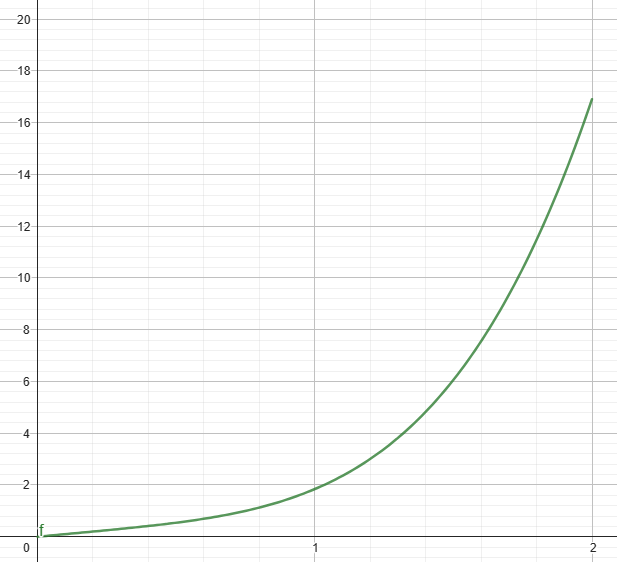
\includegraphics[width=7cm]{Images/figure_2/percobaanSatu.png}
    \caption{Grafik fungsi $f$ pada eksperimen pertama}
    \label{grafikf1}
\end{figure}

Dari Gambar \ref{grafikf1} diperoleh fungsi $f$ merupakan fungsi yang kontinu pada interval $[0,2]$. Eksperimen dengan menginterpolasi titik pada fungsi $f$, dilakukan untuk mengamati tingkat akurasi metode ketika menginterpolasi fungsi kontinu.
\subsection{Interval Sama Besar}

Untuk membagi interval $[0,2]$ menjadi beberapa interval sama besar dibentuk titik-titik $x_j^l = j/2^l, ~ j=0,\dots,2^{l+1}$, dengan $l$ suatu bilangan bulat positif. Dari titik-titik tersebut dibentuk subinterval-subinterval pada interval $[0,2]$ berupa $[x_j^l, x_{j+1}^l], ~ j=0,\dots,2^{l+1}-1$. Pada setiap interval tersebut akan dilakukan interpolasi spline kubik dengan metode yang sudah diberikan sebelumnya.

Pada metode $\textbf{O}$ dan $\textbf{R}$, $\dot{f}_{2^l}$ akan ditentukan dengan metode nonlinear pada Persamaan \eqref{dotf_FB} dan Persamaan \eqref{dotf_AY}. Hal ini dilakukan dengan menganggap syarat monoton tidak terpenuhi pada indeks $i_0 = 2^l$.

Pertama ditinjau eksperimen pertama dengan mendefinisikan $$W = \{ i : 0 \leq i \leq 2^{l+1}\}.$$ Dengan $W$ yang telah didefinisikan tersebut diperoleh estimasi order akurasi pada tabel berikut.

\begin{table}[htp]
        \centering
        \resizebox{16cm}{!}{\begin{tabular}{|c|c|c|c|c|c|}
    \hline h&$\textbf{S}$&$\textbf{O}_{FB}$&$\textbf{O}_{AY}$&$\textbf{R}_{FB}$&$\textbf{R}_{AY}$ \\ 
    \hline
0.03125&4.091080527603661&1.0052313175598333&2.099843529653508&1.0052313175598333&2.099843529653508 \\
0.015625&4.045316716039749&1.0056686933733154&2.051216705139928&1.0056686933733154&2.051216705139928 \\
0.0078125&4.022597338607468&1.0035536287913114&2.0259355147706732&1.0035536287913114&2.0259355147706732 \\
0.00390625&4.0110567600947284&1.0019515392034994&2.0130499424713526&1.0019515392034994&2.0130499424713526 \\
    \hline
    \end{tabular}}
        \caption{Tabel estimasi order akurasi eksperimen pertama dengan interval sama besar $h=2^{-l}$, $5 \leq l \leq 8$, $W = \{ i : 0 \leq i \leq 2^{l+1}\}$}
        \label{tabel1}
    \end{table}
    
Pada Tabel \ref{tabel1} metode yang memiliki order akurasi paling tinggi adalah $\textbf{S}$ dikarenakan setiap intervalnya sama besar sehingga berdasarkan Teorema \ref{oa4} order akurasi dari pendekatan turunan pertama setiap titiknya memiliki tingkat akurasi order keempat. Untuk metode yang lain order akurasinya mengikuti order akurasi dari metode nonlinear yang digunakan untuk menggantikan $f_{i_0}$, hal ini sesuai dengan Proposisi \ref{proposisi4.3.1} dan Akibat \ref{crlyR} sehingga metode $\textbf{O}_{FB}$ dan $\textbf{R}_{FB}$ memiliki tingkat akurasi order pertama sedangkan metode $\textbf{O}_{AY}$ dan $\textbf{R}_{AY}$ memiliki tingkat akurasi order kedua.

Selanjutnya, akan diamati order akurasi dari turunan pertama setiap metode pada titik selain titik $i_0$. Didefinisikan himpunan indeks $$W = \{ i : 0 \leq i \leq 2^{l+1} \} \backslash \{i_0\} ,$$ sehingga diperoleh tabel estimasi order akurasi sebagai berikut.

\begin{table}[htp]
        \centering
        \resizebox{16cm}{!}{\begin{tabular}{|c|c|c|c|c|c|}
    \hline h&$\textbf{S}$&$\textbf{O}_{FB}$&$\textbf{O}_{AY}$&$\textbf{R}_{FB}$&$\textbf{R}_{AY}$ \\ 
    \hline
0.03125&4.091080527603661&4.091080527603661&4.091080527603661&1.0052340605970105&2.099826586423638 \\
0.015625&4.045316716039749&4.045316716039749&4.045316716039749&1.0056690098407222&2.0512120412636876 \\
0.0078125&4.022597338607468&4.022597338607468&4.022597338607468&1.00355366690459&2.025934296106978 \\
0.00390625&4.0110567600947284&4.0110567600947284&4.0110567600947284&1.0019515438848565&2.0130496269743565\\
    \hline
    \end{tabular}}
        \caption{Tabel estimasi order akurasi eksperimen pertama dengan interval sama besar $h=2^{-l}$, $5 \leq l \leq 8$, $W = \{ i : 0 \leq i \leq 2^{l+1} \} \backslash \{i_0\}$}
        \label{tabel2}
    \end{table}

Dengan memperhatikan setiap titik selain titik $i_0$ diperoleh hasil estimasi order akurasinya seperti yang ada pada Tabel \ref{tabel2} dengan metode $\textbf{O}$ yang hanya mengganti pendekatan turunan pertama pada titik $i_0$ memiliki order akurasi sama dengan metode $\textbf{S}$ sesuai dengan Proposisi \ref{proposisi4.3.1}. Sedangkan untuk metode $\textbf{R}$ estimasi order akurasinya hampir tidak mengalami perubahan.

Berdasarkan Akibat \ref{crlyR} dapat dibentuk 
\begin{align*}
    W_3=\{ i : 1\leq i \leq l_0 \text{ atau } l_1 \leq i \leq 2^{l+1} - 1\},
\end{align*} 
dengan
\begin{align*}
    l_0 = (i_0 - 1) + \log_2(\hat{h}) = (2^l - 1) + \log_2(2^{-l}) = 2^l - l - 1,\\
    l_1 = (i_0 + 1) - \log_2(\hat{h}) = (2^l + 1) - \log_2(2^{-l}) = 2^l + l + 1,
\end{align*}
sehingga diperoleh estimasi order akurasi pada himpunan indeks $W$ sebagai berikut.

\begin{table}[htp]
        \centering
        \resizebox{16cm}{!}{\begin{tabular}{|c|c|c|c|c|c|}
    \hline h&$\textbf{S}$&$\textbf{O}_{FB}$&$\textbf{O}_{AY}$&$\textbf{R}_{FB}$&$\textbf{R}_{AY}$ \\ 
    \hline
0.03125&4.091080527603661&4.091080527603661&4.091080527603661&2.905982103081887&3.9933604367881785 \\
0.015625&4.045316716039749&4.045316716039749&4.045316716039749&2.905397596968384&3.9589229739193574 \\
0.0078125&4.022597338607468&4.022597338607468&4.022597338607468&2.9036663348820766&3.919322529589285 \\
0.00390625&4.0110567600947284&4.0110567600947284&4.0110567600947284&2.901862424090919&3.919632830156327\\
    \hline
    \end{tabular}}
        \caption{Tabel estimasi order akurasi eksperimen pertama dengan interval sama besar $h=2^{-l}$, $5 \leq l \leq 8$, $W=\{ i : 1\leq i \leq l_0 $ atau $l_1 \leq i \leq 2^{l+1}- 1\}$, $l_0 = 2^l - l - 1$ dan $l_1 =  2^l + l + 1$}
        \label{tabel3}
    \end{table}

Pada Tabel \ref{tabel3} hasil estimasi order akurasi untuk metode $\textbf{R}$ mengalami peningkatan. Sebelumnya, metode $\textbf{R}_{FB}$ memiliki tingkat akurasi order pertama lalu meningkat menjadi order ketiga. Lalu menggunakan metode $\textbf{R}_{AY}$ diperoleh tingkat akurasi order keempat. Dari hasil yang diproleh dapat disimpulkan bahwa interpolasi kubik spline yang diperoleh akan memiliki order akurasi optimal pada $[x_1, x_{l_0}] \cap [x_{l_1}, x_n]$ sesuai dengan Lema \ref{orderAkurasi}.

\subsection{Interval Tidak Sama Besar}

Untuk experimen ketika interval yang didefinisikan tidak sama besar dibentuk titik-titik
\begin{align*}
    x_{2j}^l = 2^{-l}j,\\
    x_{2j + 1}^l = 2^{-l}(j + \frac{1}{4}),
\end{align*}
dengan $j = 0,~1,\dots,~2^{l+1}$ sehingga $x_{2^{l+2}}^l = 2$ untuk suatu $l$ bilangan bulat positif. Subinterval yang dibentuk dari titik-titik tersebut memiliki besar interval terbesar $\hat{h}=\frac{3}{4}2^{-l}$. Sama seperti pada saat membagi interval menjadi sama besar, diangga syarat monoton tidak terpenuhi pada saat $x_i^l=1$ sehingga diperoleh $i_0 = 2^{l+1}$.

Diperhatikan bahwa apabila dipilih $l+1$ sebagai bilangan bulat dalam menentukan titik-titiknya, maka titik tepat setelah titik $x_{1_0}^l$ yaitu $x_{2^{l+1}+1}^l$ tidak termuat dalam titik-titik yang dibentuk dengan memilih $l+1$ sebagai bilangan bulatnya. Akan tetapi, ketika dipilih $l+2$ sebagai bilangan bulat dalam menentukan titik-titiknya diperoleh titik $x_{2^{l+3}+2}^{l+2}$ merupakan titik yang sama dengan $x_{2^{l+1}+1}^l$ dikarenakan
\begin{align*}
    x_{2^{l+1}+1}^l = 2^{-l}(2^l + \frac{1}{4}) = 2^{-l}( \frac{2^{l+2} + 1}{4}) = 2^{-(l+2)}(2^{l+2} + 1) = x_{2(2^{l+2}+1)}^{l+2} = x_{2^{l+3}+2}^{l+2}.
\end{align*}
Berdasarkan hal tersebut maka untuk mengestimasi order akurasinya digunakan
\begin{align*}
    \Tilde{o}_l^W := \log_4(\frac{e_{l}^W}{e_{l-2}^W}).
\end{align*}

Ditinjau pada eksperimen pertama dengan mendefinisikan $$W = \{ i : 0 \leq i \leq 2^{l+2}\}.$$ Dengan $W$ yang telah didefinisikan tersebut diperoleh estimasi order akurasi pada tabel berikut.

\begin{table}[htp]
        \centering
        \resizebox{16cm}{!}{\begin{tabular}{|c|c|c|c|c|c|}
    \hline $\hat{h}$&$\textbf{S}$&$\textbf{O}_{FB}$&$\textbf{O}_{AY}$&$\textbf{R}_{FB}$&$\textbf{R}_{AY}$ \\ 
    \hline
0.09375&2.9759259549890644&1.1996206110220025&1.9674933943413442&1.1996206110220025&1.9674933943413442 \\
0.0234375&2.9998036042499936&1.0791057503379433&2.0074308008422164&1.0791057503379433&2.0074308008422164 \\
0.005859375&2.9999935454809488&1.0220158560654877&2.002717768406527&1.0220158560654877&2.002717768406527 \\
0.00146484375&2.997839181332225&1.0056537201758062&2.00073084478135&1.0056537201758062&2.00073084478135\\
    \hline
    \end{tabular}}
        \caption{Tabel estimasi order akurasi eksperimen pertama dengan interval tidak sama besar $\hat{h}=\frac{3}{4}2^{-l}$, $l \in \{3,5,7,9\}$, $W=\{ i : 0\leq i \leq 2^{l+2} \}$}
        \label{tabel4}
    \end{table}

Pada Tabel \ref{tabel4} metode $\textbf{S}$ memiliki tingkat akurasi order ketiga. Hal ini sesuai dengan Teorema \ref{3.3.3} karena besar intervalnya tidak sama besar. Untuk metode yang lainnya order akurasi ditentukan oleh metode nonlinear yang digunakan untuk mengestimasi turunan pertama pada indeks $i_0$ sesuai dengan Proposisi \ref{proposisi4.3.1} dan Akibat \ref{crlyR}.

Seperti pada kasus intervalnya sama besar, akan diamati titik-titik selain titik yang berkorespondensi dengan indeks $i_0$. Untuk mengamati titik tersebut didefinisikan $$W = \{ i : 0 \leq i \leq 2^{l+2}\} \backslash \{i_0\},$$ sehingga diperoleh estimasi order akurasinya sebagai berikut.

\begin{table}[htp]
        \centering
        \resizebox{16cm}{!}{\begin{tabular}{|c|c|c|c|c|c|}
    \hline $\hat{h}$&$\textbf{S}$&$\textbf{O}_{FB}$&$\textbf{O}_{AY}$&$\textbf{R}_{FB}$&$\textbf{R}_{AY}$ \\ 
    \hline
0.09375&2.9714330778182014&2.9902764530272874&2.9902764530272874&1.1622746297064157&1.9189743367447858 \\
0.0234375&2.9998036042499936&2.999910004840339&2.999910004840339&1.0760473705263671&1.9963910348993905 \\
0.005859375&2.9999935454809488&2.9999935454809488&2.9999935454809488&1.0218020986447498&1.9999539282161043 \\
0.00146484375&2.997839181332225&2.997839181332225&2.997839181332225&1.005639931922115&2.0000385644786993\\
    \hline
    \end{tabular}}
        \caption{Tabel estimasi order akurasi eksperimen pertama dengan interval tidak sama besar $\hat{h}=\frac{3}{4}2^{-l}$, $l \in \{3,5,7,9\}$, $W=\{ i : 0\leq i \leq 2^{l+2} \} \backslash \{i_0\}$}
        \label{tabel5}
    \end{table}

Pada Tabel \ref{tabel5} metode $\textbf{O}$ memiliki order akurasi yang hampir sama dengan metode $\textbf{S}$ sebagaimana yang diberikan pada Proposisi \ref{proposisi4.3.1}. Hal ini disebabkan metode $\textbf{O}$ hanya mengganti estimasi turunan pertama dengan menggunakan metode nonlinear pada titik $x_{i_0}^l$ saja. Sedangkan untuk metode $\textbf{R}$ estimasi order akurasi tidak banyak mengalami perubahan.

Diperhatikan, berdasarkan Proposisi \ref{proposisi4.3.1} terdapat $l_0$ dan $l_1$ sehingga dapat dibentuk himpunan
\begin{align*}
    W = \{ i : 1 \leq i \leq l_0 \text{ atau } l_1 \leq i \leq 2^{l+2} - 1 \},
\end{align*}
dengan
\begin{align*}
    l_0 = (i_0 - 1) + \log_2(\hat{h}) = (2^{l+1} - 1) + \log_2(\frac{3}{4} 2^{-l}), \\
    l_1 = (i_0 + 1) - \log_2(\hat{h}) = (2^{l+1} + 1) - \log_2(\frac{3}{4} 2^{-l}),
\end{align*}
sehingga diperoleh hasil estimasi order akurasi pada tabel berikut.

\begin{table}[htp]
        \centering
        \resizebox{16cm}{!}{\begin{tabular}{|c|c|c|c|c|c|}
    \hline $\hat{h}$&$\textbf{S}$&$\textbf{O}_{FB}$&$\textbf{O}_{AY}$&$\textbf{R}_{FB}$&$\textbf{R}_{AY}$ \\ 
    \hline
0.0234375&2.9998036042499936&2.999910004840339&2.999910004840339&2.9996523221646325&2.999758815318022 \\
0.005859375&2.9999935454809488&2.9999935454809488&2.9999935454809488&2.9999935459109084&2.9999935459109084 \\
0.00146484375&2.997839181332225&2.997839181332225&2.997839181332225&2.997839181332225&2.997839181332225 \\
    \hline
    \end{tabular}}
        \caption{Tabel estimasi order akurasi eksperimen pertama dengan interval tidak sama besar $\hat{h}=\frac{3}{4}2^{-l}$, $l \in \{3,5,7,9\}$, $W = \{ i : 1 \leq i \leq l_0 \text{ atau } l_1 \leq i \leq 2^{l+2} - 1 \}$, $l_0 = (2^{l+1} - 1) + \log_2(\frac{3}{4} 2^{-l})$ dan $l_1 = (2^{l+1} + 1) - \log_2(\frac{3}{4} 2^{-l})$}
        \label{tabel6}
    \end{table}

Diperhatikan bahwa untuk $l = 1$ diperoleh $l_0 = -2.41504$ dan $l_1 = 10.41504$ sehingga $W = \emptyset$ berakibat order akurasinya tidak dapat diestimasi ketika $l = 3$. Dari Tabel \ref{tabel6} ketika beberapa titik disekitar indeks $i_0$ diabaikan diperoleh semua metode menghasilkan order akurasi yang optimal. Bahkan metode $\textbf{R}_{FB}$ menghasilkan tingkan akurasi order ketiga bukan order kedua seperti yang diprediksi oleh Akibat \ref{crlyR}.

\section{Eksperimen Kedua}

Pada eksperimen kedua fungsi yang akan diinterpolasi merupakan fungsi yang mulus sepotong-sepotong dan tidak kontinu pada satu titik. Fungsi yang tidak kontinu menyebabkan hasil interpolasi spline kubik secara umum dari fungsi tersebut tidak memiliki sifat monoton saat mendekati titik di mana fungsinya tidak kontinu.

Diberikan fungsi
\begin{align*}
    g(x) = \begin{cases}
    x^4 + \sin(x), \quad & 0\leq x \leq 1,\\
    4 + x^4 + \cos(x), \quad & 1 < x \leq 2,
    \end{cases}
\end{align*}
yang akan diinterpolasikan pada titik-titik di dalam interval $[0,2]$. Dalam menginterpolasikan fungsi tersebut pertama akan ditinjau ketika interval $[0,2]$ dibagi menjadi beberapa subinterval yang sama besar. Selanjutnya juga akan ditinjau ketika intervalnya dibagi menjadi subinterval yang tidak sama besar. 

\begin{figure}[H]
    \centering
    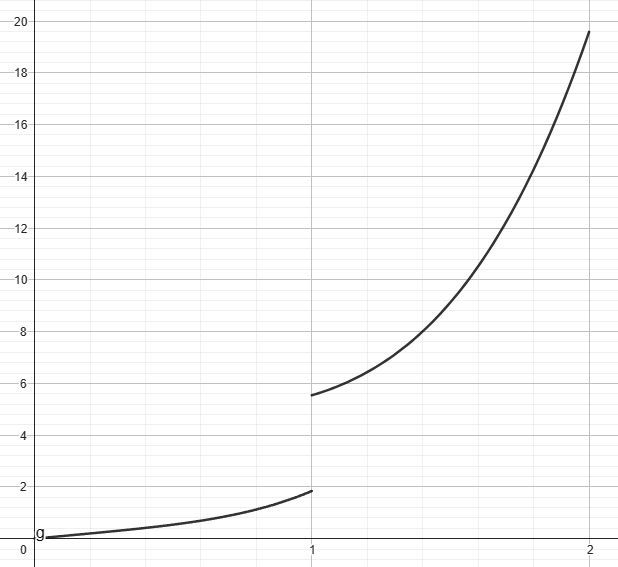
\includegraphics[width=7cm]{Images/figure_2/percobaanDua.png}
    \caption{Grafik fungsi $g$ pada eksperimen kedua}
    \label{grafikg2}
\end{figure}

Dari Gambar \ref{grafikg2} dapat dilihat bahwa fungsi $g$ tidak kontinu pada titik \mbox{$x=1$}. Eksperimen kedua dilakukan untuk mengamati tingkat akurasi metode ketika menginterpolasi fungsi yang tidak kontinu.

\subsection{Interval Sama Besar}
Dibentuk titik-titik pada interval $[0,2]$ berupa $x_j^l = j/2^l, ~ j=0,\dots,2^{l+1}$, dengan $l$ suatu bilangan bulat positif yang sudah ditentukan. Interval yang dibentuk di antara titik-titik yang dibentuk memiliki interval yang sama besar yaitu $h = 2^{-l}$. Berikut adalah grafik dan plot dari galat yang diperoleh jika dipilih $l = 4$ sehingga intervalnya sama besar yaitu $h=0.625$. 

Pada experimen titik-titik yang estimasi turunan pertamanya ditentukan dengan menggunakan metode nonlinear pada metode $\textbf{O}$ adalah titik-titik pada indeks $\{2^l-1, 2^l, 2^l+1, 2^l+2\}$ sedangkan pada metode $\textbf{R}$ titik-titik yang ditentukan estimasi turunan pertamanya menggunakan metode nonlinear adalah titik-titik pada indeks $\{2^l, 2^l+1\}$. Titik ini dipilih untuk mengamati perubahan nilai akurasi yang diperoleh dari kedua metode apabila panjang interval berubah-ubah.

\begin{figure}[H]
    \centering
    \raisebox{1.5cm}{\rotatebox[origin=t]{90}{$\textbf{S}$}}
    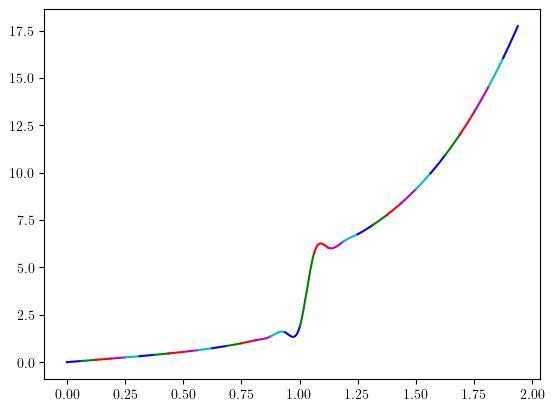
\includegraphics[width=5cm]{Images/figure_2/grafikS2.png}
    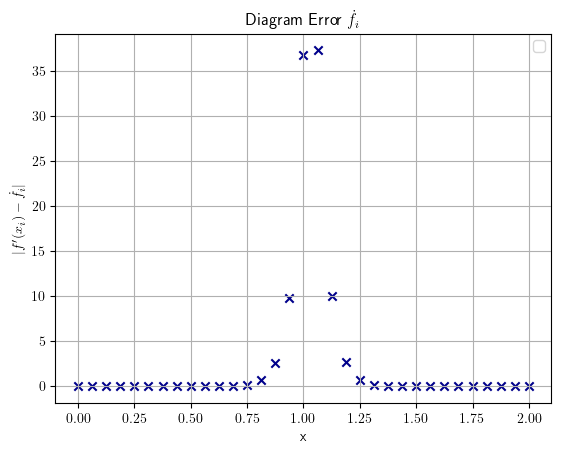
\includegraphics[width=5cm]{Images/figure_2/plotS2.png}
\end{figure}

\begin{figure}[H]
    \centering
    \raisebox{1.5cm}{\rotatebox[origin=t]{90}{$\textbf{O}_{FB}$}}
    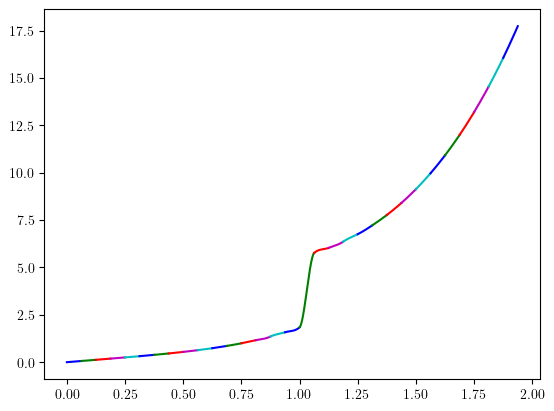
\includegraphics[width=5cm]{Images/figure_2/grafikOFB2.png}
    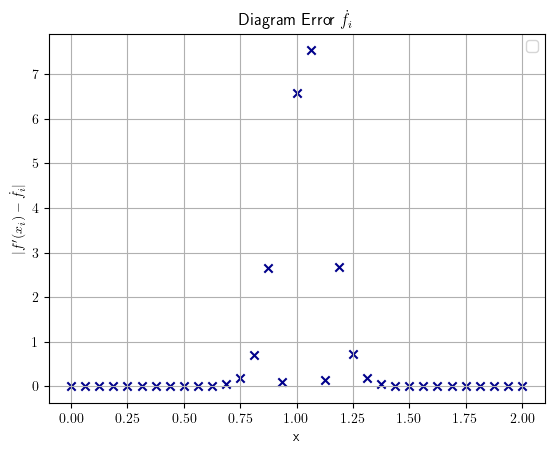
\includegraphics[width=5cm]{Images/figure_2/plotOFB2.png}
    \\
    \raisebox{1.5cm}{\rotatebox[origin=t]{90}{$\textbf{O}_{AY}$}}
    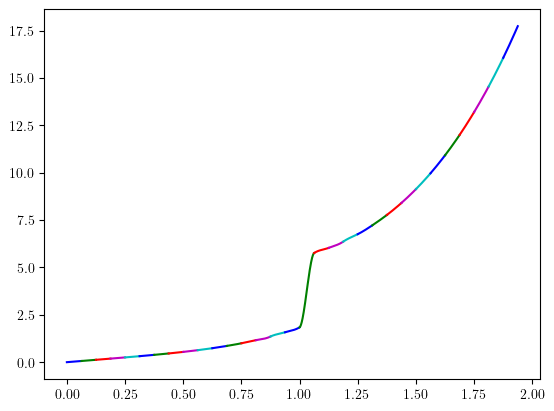
\includegraphics[width=5cm]{Images/figure_2/grafikOAY2.png}
    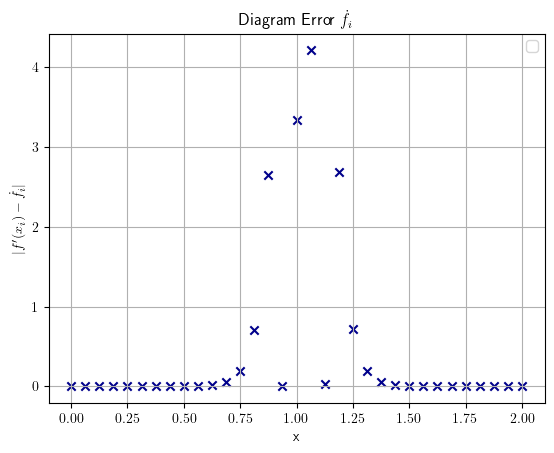
\includegraphics[width=5cm]{Images/figure_2/plotOAY2.png}
    \\
    \raisebox{1.5cm}{\rotatebox[origin=t]{90}{$\textbf{R}_{FB}$}}
    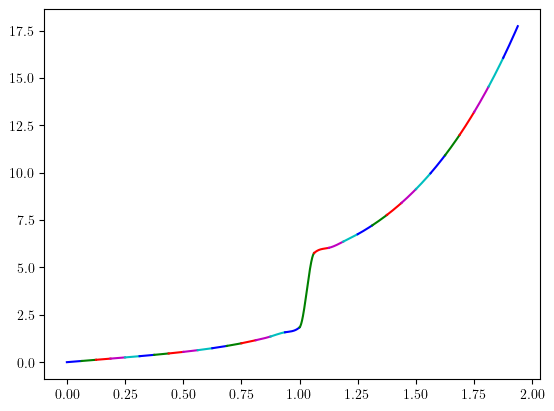
\includegraphics[width=5cm]{Images/figure_2/grafikRFB2.png}
    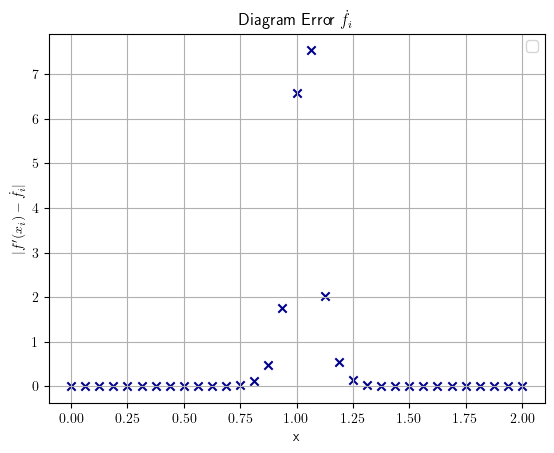
\includegraphics[width=5cm]{Images/figure_2/plotRFB2.png}
    \\
    \raisebox{1.5cm}{\rotatebox[origin=t]{90}{$\textbf{R}_{AY}$}}
    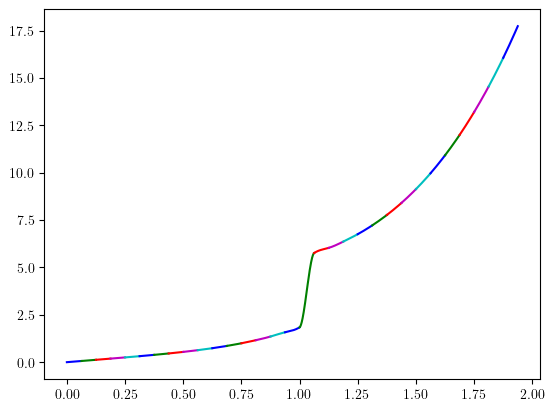
\includegraphics[width=5cm]{Images/figure_2/grafikRAY2.png}
    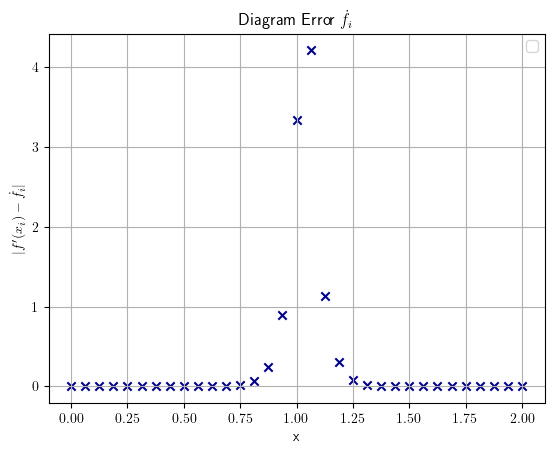
\includegraphics[width=5cm]{Images/figure_2/plotRAY2.png}
    \caption{Eksperimen kedua dengan $l=4$ interval sama besar}
    \label{grafikPlot2}
\end{figure}

    Pada Gambar \eqref{grafikPlot2} terlihat metode $\textbf{O}$ dan $\textbf{R}$ masing-masing menghasilkan hasil interpolasi yang monoton pada interval disekitar titik $x=1$ sedangkan metode $\textbf{S}$ mengalami osilasi pada hasil interpolasi saat mendekati titik $x=1$ di mana fungsi yang diinterpolasi tidak kontinu menyebabkan syarat monotonnya tidak terpenuhi. Selain itu galat dari hasil pendekatan turunan pertama yang dihasilkan dengan metode $\textbf{S}$ relatif sangat besar ketika mendekati titik $x=1$ dibandingkan dengan metode yang lainnya. Dapat dilihat juga galat yang diperoleh ketiga menggunakan metode nonlinear $FB$ menghasilkan galat yang lebih besar hingga dua kali galat ketika menggunakan metode $AY$.

    Perlu diperhatikan bahwa untuk eksperimen kedua pada titik $i_0 = 2^l$ syarat monoton selalu tidak terpenuhi karena pada titik fungsi yang diinterpolasi tidak kontinu pada interval $[x_{2^{l}}, x_{2^l + 1}]$. Berdasarkan Proposisi \ref{prpsslast} dengan $r=1$ didefinisikan himpunan indeks
    $$W=\{ i : 1\leq i \leq l_0 \text{ atau } l_1 \leq i \leq 2^{l+1} - 1\},$$ 
    dengan
    \begin{align*}
        l_0 = (i_0 - 1) + \log_2(\hat{h}) = (2^l - 1) + \log_2(2^{-l}) = 2^l - l - 1,\\
        l_1 = (i_0 + 1) - \log_2(\hat{h}) = (2^l + 1) - \log_2(2^{-l}) = 2^l + l + 2,
    \end{align*}
    berakibat diperoleh tabel estimasi order akurasinya sebagai berikut.

    \begin{table}[htp]
        \centering
        \resizebox{16cm}{!}{\begin{tabular}{|c|c|c|c|c|c|}
    \hline h&$\textbf{S}$&$\textbf{O}_{FB}$&$\textbf{O}_{AY}$&$\textbf{R}_{FB}$&$\textbf{R}_{AY}$ \\ 
    \hline
0.03125&0.896372535576625&0.896372535576625&0.896372535576625&2.9661347200468837&3.945353043785682 \\
0.015625&0.8981807720392228&0.8981807720392228&0.8981807720392228&2.934978479747872&3.925153321202357 \\
0.0078125&0.8990766668112026&0.8990766668112026&0.8990766668112026&2.918177295769085&3.91032575666795 \\
0.00390625&0.8995232015410665&0.8995232015410665&0.8995232015410665&2.9091723530199505&3.9071945357648943 \\
    \hline
    \end{tabular}}
        \caption{Tabel estimasi order akurasi eksperimen kedua dengan interval sama besar $h=2^{-l}$, $5 \leq l \leq 8$, $W=\{ i : 1\leq i \leq l_0 $ atau $l_1 \leq i \leq 2^{l+1}- 1\}$, $l_0 = 2^l - l - 1$ dan $l_1 =  2^l + l + 2$}
        \label{tabel7}
    \end{table}

    Dari Tabel \ref{tabel7} dapat disimpulkan bahwa metode $\textbf{O}$ mengalami penurunan akurasi lebih besar dari pada metode $\textbf{R}$ pada area disekitar $[x_{2^{l}}, x_{2^l+1}]$. Seperti sebelumnya dengan memanfaatkan Proposisi \ref{prpsslast} dan $r=2$ dibentuk himpunan yang lebih kecil berupa 
    $$W=\{ i : 1\leq i \leq l_0 \text{ atau } l_1 \leq i \leq 2^{l+1} - 1\},$$ 
    dengan
    \begin{align*}
        l_0 = (i_0 - 1) + 2\log_2(\hat{h}) = (2^l - 1) + 2\log_2(2^{-l}) = 2^l - 2l - 1,\\
        l_1 = (i_0 + 1) - 2\log_2(\hat{h}) = (2^l + 1) - 2\log_2(2^{-l}) = 2^l + 2l + 2,
    \end{align*}
    sehingga diperoleh estimasi order akurasi pada area tersebut pada tabel berikut.
    
    \begin{table}[htp]
        \centering
        \resizebox{16cm}{!}{\begin{tabular}{|c|c|c|c|c|c|}
    \hline h&$\textbf{S}$&$\textbf{O}_{FB}$&$\textbf{O}_{AY}$&$\textbf{R}_{FB}$&$\textbf{R}_{AY}$ \\ 
    \hline
0.03125&2.7960799781563304&2.7960799781563304&2.7960799781563304&4.8390922004107555&6.043717175770229 \\
0.015625&2.798034660598472&2.798034660598472&2.798034660598472&4.793213617610702&4.457115286101313 \\
0.0078125&2.7989979341003295&2.7989979341003295&2.7989979341003295&4.750282195219751&3.999927133695036 \\
0.00390625&2.79947361166368&2.79947361166368&2.79947361166368&4.673930753027552&3.957318743784382 \\
    \hline
    \end{tabular}}
        \caption{Tabel estimasi order akurasi eksperimen kedua dengan interval sama besar $h=2^{-l}$, $5 \leq l \leq 8$, $W=\{ i : 1\leq i \leq l_0 $ atau $l_1 \leq i \leq 2^{l+1}- 1\}$, $l_0 = 2^l - 2l - 1$ dan $l_1 =  2^l + 2l + 2$}
        \label{tabel8}
    \end{table}

    Tabel \ref{tabel8} memberikan estimasi order akurasi pada area yang lebih jauh dari titik $x=1$ di mana titik tidak kontinu. Dari hasil yang diperoleh, metode $\textbf{S}$, metode $\textbf{O}$, dan metode $\textbf{R}$ menghasilkan order akurasi yang lebih baik semakin menjauhi titik $x=1$ di mana fungsi yang diinterpolasi mengalami ketidak kontinuan.
    
\subsection{Interval Tidak Sama Besar}

Sama seperti pembuatan subinterval yang tidak sama besar pada eksperimen pertama dibentuk titik-titik
\begin{align*}
    x_{2j}^l = 2^{-l}j,\\
    x_{2j + 1}^l = 2^{-l}\left(j + \frac{1}{4}\right),
\end{align*}
dengan $j = 0,~1,\dots,~2^{l+1}$ sehingga diperoleh untuk suatu bilangan bulat $l$ subinterva-subinterval yang terbentuk di antara titik-titiknya memiliki interval terbesar \mbox{$\hat{h} = \frac{3}{4}2^{-l}.$} Dengan mengambil $l=3$, maka diperoleh grafik hasil interpolasi dan plot galat turunan pertama disetiap titik berikut.

\begin{figure}[H]
    \centering
    \raisebox{1.5cm}{\rotatebox[origin=t]{90}{$\textbf{S}$}}
    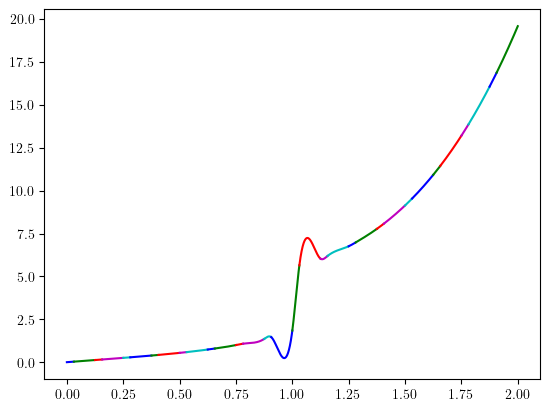
\includegraphics[width=6cm]{Images/figure_2/grafikS2n.png}
    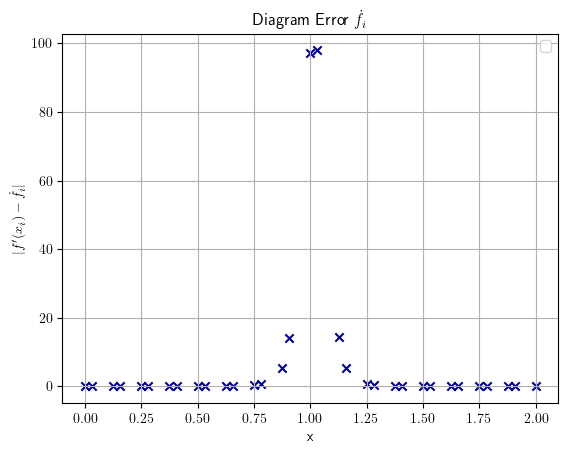
\includegraphics[width=6cm]{Images/figure_2/plotS2n.png}
\end{figure}

\begin{figure}[H]
    \centering
    \raisebox{1.5cm}{\rotatebox[origin=t]{90}{$\textbf{O}_{FB}$}}
    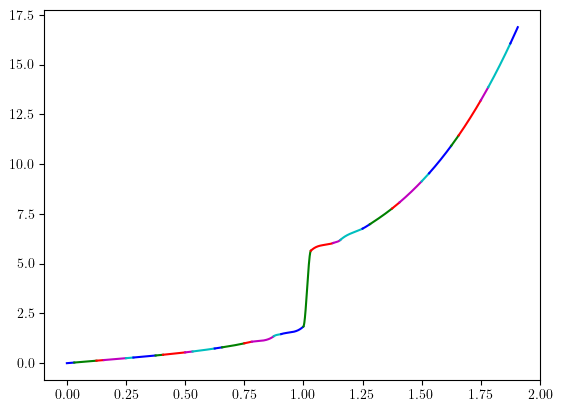
\includegraphics[width=6cm]{Images/figure_2/grafikOFB2n.png}
    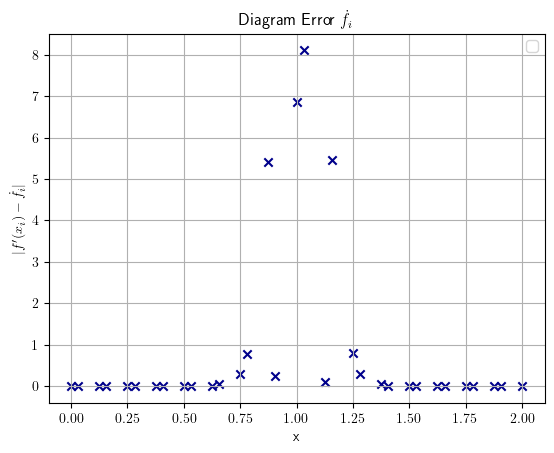
\includegraphics[width=6cm]{Images/figure_2/plotOFB2n.png}
    \\
    \raisebox{1.5cm}{\rotatebox[origin=t]{90}{$\textbf{O}_{AY}$}}
    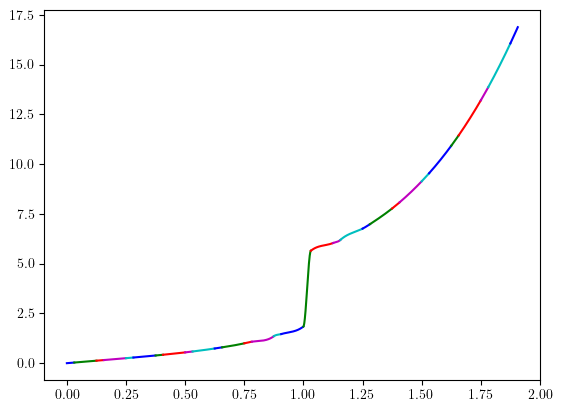
\includegraphics[width=6cm]{Images/figure_2/grafikOAY2n.png}
    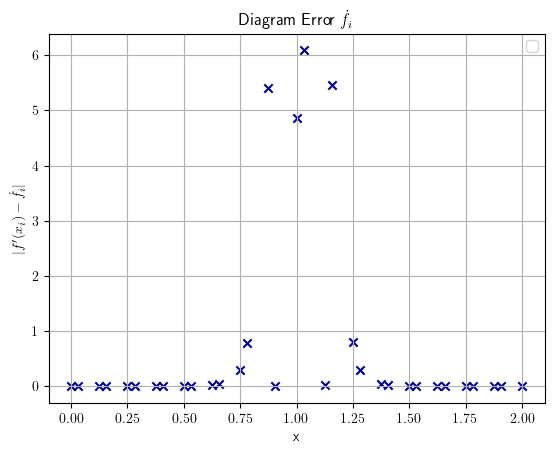
\includegraphics[width=6cm]{Images/figure_2/plotOAY2n.png}
    \\
    \raisebox{1.5cm}{\rotatebox[origin=t]{90}{$\textbf{R}_{FB}$}}
    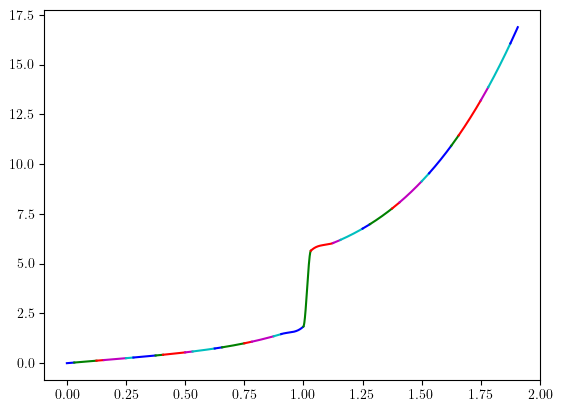
\includegraphics[width=6cm]{Images/figure_2/grafikRFB2n.png}
    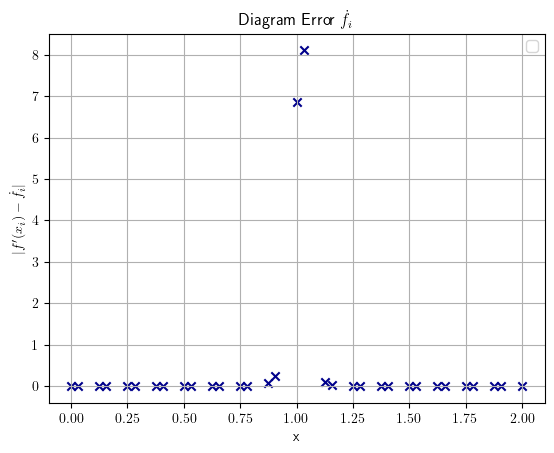
\includegraphics[width=6cm]{Images/figure_2/plotRFB2n.png}
    \\
    \raisebox{1.5cm}{\rotatebox[origin=t]{90}{$\textbf{R}_{AY}$}}
    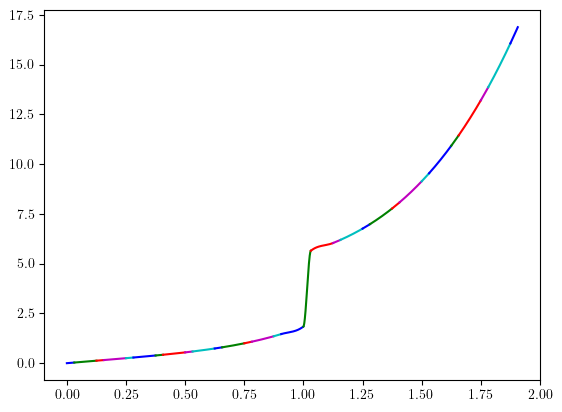
\includegraphics[width=6cm]{Images/figure_2/grafikRAY2n.png}
    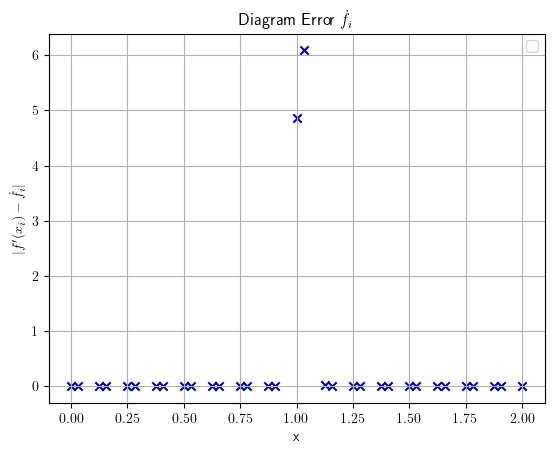
\includegraphics[width=6cm]{Images/figure_2/plotRAY2n.png}
    \caption{Eksperimen kedua dengan $l=4$ interval tidak sama besar}
    \label{grafikPlot2n}
\end{figure}

Gambar \eqref{grafikPlot2n} memberikan grafik fungsi interpolasi dan plot galat turunan dari setiap metode. Dari hasil plot tersebut dapat disimpulkan metode $\textbf{R}$ memberikan hasil pendekatan turunan pada sekitar titik tidak kontinu dengan galat yang paling kecil dibandingkan dengan metode lainnya.

Untuk mengamati order akurasi dari turunan pertama disekitar titik $x=1$ didefinisikan himpunan indeks
\begin{align*}
    W = \{ i: 0 \leq i \leq l_0 \text{ atau } l_1 \leq i \leq 2^{l+2} \},
\end{align*}
dengan
\begin{align*}
    l_0 = (i_0 - 1) + \log_2(\hat{h}) = (2^{l+1} - 1) + \log_2\left(\frac{3}{4} 2^{-l}\right), \\
    l_1 = (i_0 + 1) - \log_2(\hat{h}) = (2^{l+1} + 2) - \log_2\left(\frac{3}{4} 2^{-l}\right).
\end{align*}
Estimasi order akurasi yang digunakan sama seperti pada eksperimen pertama yaitu menggunakan
\begin{align*}
    \Tilde{o}_l^W := \log_4\left(\frac{e_{l}^W}{e_{l-2}^W}\right).
\end{align*}
Dengan mengamati titik-titik tersebut maka diperoleh hasil estimasi order akurasi sebagai berikut.

\begin{table}[htp]
        \centering
        \resizebox{16cm}{!}{\begin{tabular}{|c|c|c|c|c|c|}
    \hline h&$\textbf{S}$&$\textbf{O}_{FB}$&$\textbf{O}_{AY}$&$\textbf{R}_{FB}$&$\textbf{R}_{AY}$ \\ 
    \hline
0.0234375&1.0791206523482317&1.0791206523482317&1.0791206523482317&2.016816138147151&2.955130599603732 \\
0.005859375&1.0823271429167844&1.0823271429167844&1.0823271429167844&1.7387074723422433&3.024111952732935 \\
0.00146484375&1.0826615986711732&1.0826615986711732&1.0826615986711732&2.3353545234629536&2.9913528591017755 \\
    \hline
    \end{tabular}}
        \caption{Tabel estimasi order akurasi eksperimen kedua dengan interval tidak sama besar $\hat{h}=\frac{3}{4}2^{-l}$, $5 \leq l \leq 8$, $W=\{ i : 1\leq i \leq l_0 $ atau $l_1 \leq i \leq 2^{l+1}- 1\}$, $l_0 = (2^{l+1} - 1) + \log_2(\frac{3}{4}2^{-l})$ dan $l_1 = (2^{l+1} + 2) - \log_2(\frac{3}{4}2^{-l})$}
        \label{tabel9}
    \end{table}

Dari Tabel \ref{tabel9} hasil estimasi order akurasi masih belum menghasilkan hasil interpolasi yang optimal pada area sekitar titik yang tidak kontinuan, baik menggunakan metode $\textbf{S}$ dan metode $\textbf{O}$. Pada metode $\textbf{R}$ order akurasi terlihat meningkat, namun belum menghasilkan interpolasi yang optimal.

Selanjutnya akan diamati untuk titik-titik yang lebih jauh dari titik di mana fungsi $g$ tidak kontinu. Dibentuk
\begin{align*}
    W = \{ i: 0 \leq i \leq l_0 \text{ atau } l_1 \leq i \leq 2^{l+2} \},
\end{align*}
dengan
\begin{align*}
    l_0 = (i_0 - 1) + 2\log_2(\hat{h}) = (2^{l+1} - 1) + 2\log_2(\frac{3}{4} 2^{-l}), \\
    l_1 = (i_0 + 1) - 2\log_2(\hat{h}) = (2^{l+1} + 2) - 2\log_2(\frac{3}{4} 2^{-l}),
\end{align*}
sehingga diperoleh hasil estimasi order akurasi pada tabel berikut
\begin{table}[htp]
        \centering
        \resizebox{16cm}{!}{\begin{tabular}{|c|c|c|c|c|c|}
    \hline h&$\textbf{S}$&$\textbf{O}_{FB}$&$\textbf{O}_{AY}$&$\textbf{R}_{FB}$&$\textbf{R}_{AY}$ \\ 
    \hline
0.0234375&3.1292610123804017&3.1292610123804017&3.1292610123804017&2.986526501124396&2.995424643389291 \\
0.005859375&3.12741868305077&3.12741868305077&3.12741868305077&2.9972376302527652&2.9974828976530117 \\
0.00146484375&3.121560690369995&3.121560690369995&3.121560690369995&2.998864243982574&2.999072449078856\\
    \hline
    \end{tabular}}
        \caption{Tabel estimasi order akurasi eksperimen kedua dengan interval tidak sama besar $\hat{h}=\frac{3}{4}2^{-l}$, $5 \leq l \leq 8$, $W=\{ i : 1\leq i \leq l_0 $ atau $l_1 \leq i \leq 2^{l+1}- 1\}$, $l_0 = (2^{l+1} - 1) + 2\log_2(\frac{3}{4}2^{-l})$ dan $l_1 = (2^{l+1} + 2) - 2\log_2(\frac{3}{4}2^{-l})$}
        \label{tabel10}
    \end{table}

Dari Tabel \ref{tabel10}, diperoleh bahwa semua metode menghasilkan pendekatan dengan tingkat akurasi order ketiga. Hal ini mengindikasikan hasil interpolasi sudah optimal berdasarkan Lema \ref{orderAkurasi} untuk titik yang jauh dari titik tidak kontinu.

\section{Eksperimen Ketiga}

Untuk eksperimen ketiga akan dicoba menginterpolasi titik-titik yang sama dengan interpolasi spline kubik pada Subbab \textbf{3.1} yaitu $(0,10)$, $(1,8.7)$, $(2,2.1)$, $(3,1.5)$, dan $(4,0.1)$. Dengan metode interpolasi yang telah dibahas sebelumnya, maka diperoleh grafik hasil interpolasi berikut
\begin{figure}[H]
    \centering
    \raisebox{1.5cm}{\rotatebox[origin=t]{90}{$\textbf{S}$}}
    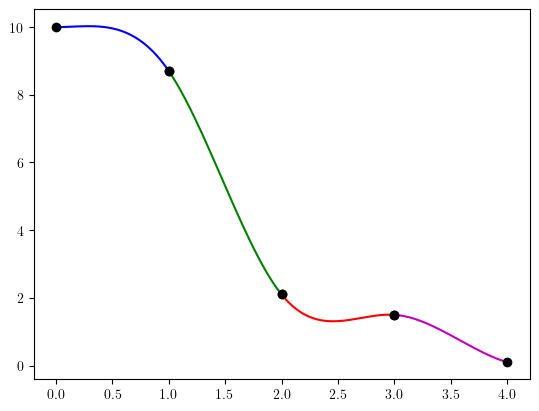
\includegraphics[width=8cm]{Images/figure_2/grafikS3.png}
\end{figure}

\begin{figure}[H]
    \centering
    \raisebox{1.5cm}{\rotatebox[origin=t]{90}{$\textbf{O}_{FB}$}}
    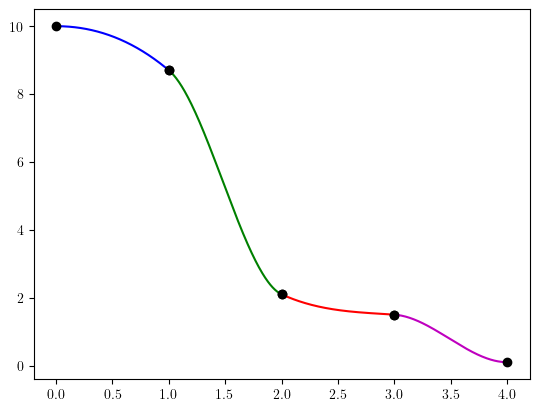
\includegraphics[width=8cm]{Images/figure_2/grafikOFB3.png}
    \\
    \raisebox{1.5cm}{\rotatebox[origin=t]{90}{$\textbf{O}_{AY}$}}
    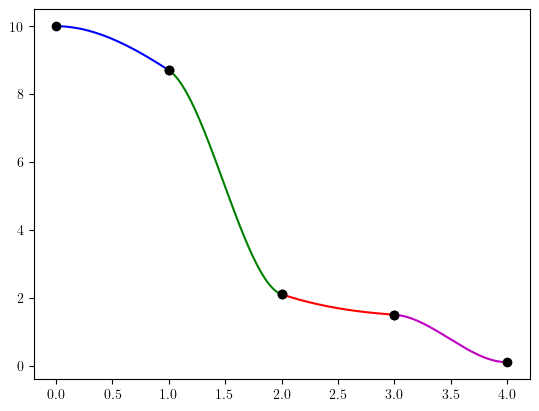
\includegraphics[width=8cm]{Images/figure_2/grafikOAY3.png}
    \\
    \raisebox{1.5cm}{\rotatebox[origin=t]{90}{$\textbf{R}_{FB}$}}
    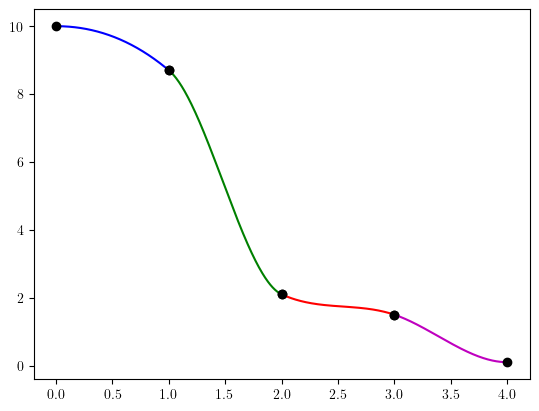
\includegraphics[width=8cm]{Images/figure_2/grafikRFB3.png}
    \\
    \raisebox{1.5cm}{\rotatebox[origin=t]{90}{$\textbf{R}_{AY}$}}
    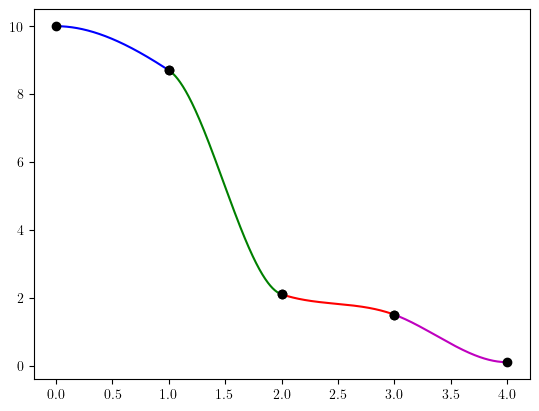
\includegraphics[width=8cm]{Images/figure_2/grafikRAY3.png}
    \caption{Eksperimen ketiga menginterpolasi titik-titik yang diberikan}
    \label{grafikPlot3}
\end{figure}

Dari Gambar \ref{grafikPlot3} diperoleh hasil interpolasi yang diperoleh monoton. Berbeda dengan hasil interpolasi sebelumnya, hasil interpolasi yang dihasilkan memiliki sifat monoton. Karena data yang diinterpolasi memiliki sifat monoton, maka hasil interpolasi yang diharapkan juga harus monoton. Hasil interpolasi yang monoton menyebabkan data hasil interpolasi yang diperoleh menjadi lebih akurat.
\chapter{KESIMPULAN}

% Kesimpulan yang dapat diambil penulis ...
Dari metode interpolasi yang telah dibahas dapat diambil kesimpulan sebagai berikut:

\begin{enumerate}
    
    \item Pada interval $[x_i,x_{i+1}]$ syarat cukup hasil interpolasi Hermite kubik monoton adalah jika $0 \leq \alpha_i, \beta_i \leq 3$,
    maka polinomial Hermite kubik yang dihasilkan memiliki sifat monoton.

    % \item Tingkat akurasi order keempat adalah order akurasi optimal dariMe interpolasi Hermite kubik yang terjadi ketika $\dot{f}_i$ dan $\dot{f}_{i+1}$ memiliki tingkat akurasi lebih dari tiga.

    \item Metode interpolasi Hermite kubik memiliki tingkat akurasi $\min(4, q_i+1, q_{i+1}+1)$ dengan
    $$\dot{f_i}=f'(x_i) + O(h^{q_i}),$$ 
    dan $$\dot{f_{i+1}}=f'(x_{i+1}) + O(h^{q_{i+1}}).$$

    \item Interpolasi spline kubik monoton berbasis polinomial Hermite kubik yang menginterpolasi titik $\{(x_i,f(x_i)): i = 0,1,\dots,n\}$ memiliki polinomial spline kubik monoton berupa
    \begin{equation*}
    P_i(x)=f_i + \dot{f}_i(x-x_i) + \frac{(m_i-\dot{f}_i)}{h_i}(x-x_i)^2 + \frac{(\dot{f}_{i+1}+\dot{f}_i-2m_i)}{h_i^2}(x-x_i)^2(x-x_{i+1}),
\end{equation*}
    dengan $\dot{f}_i$ dan $\dot{f}_{i+1}$ adalah solusi dari 
    \begin{equation*}
    \begin{bmatrix}
        2 & \mu_1 \\
        \lambda_2 & 2 & \mu_2 \\
        & \lambda_3 & 2 & \mu_3 \\
        && \ddots & \ddots & \ddots \\
        &&&\lambda_{n-3} & 2 & \mu_{n-3} \\
        &&&&\lambda_{n-2} & 2
    \end{bmatrix}
    \begin{bmatrix}
        \dot{f_2} \\
        \dot{f_3} \\
        \dot{f_4} \\
        \vdots \\
        \dot{f_{n-2}} \\
        \dot{f_{n-1}} 
    \end{bmatrix}=\begin{bmatrix}
        3(\lambda_1m_1 + \mu_1m_2) - \lambda_1f_1' \\
        3(\lambda_{2}m_{2} + \mu_{2}m_3) \\
        3(\lambda_{3}m_{3} + \mu_{3}m_4) \\
        \vdots \\
        3(\lambda_{n-3}m_{n-3} + \mu_{n-3}m_{n-2}) \\
        3(\lambda_{n-2}m_{n-2} + \mu_{n-2}m_{n-1}) - \mu_{n-2}f_n' \\
    \end{bmatrix},
\end{equation*}
    serta $\dot{f}_0 = f'(x_0)$ dan $\dot{f}_n = f'(x_n)$.

    \item Metode interpolasi spline kubik dengan basis polinomial Hermite kubik memiliki tingkat akurasi order keempat jika setiap subinterval panjangnya sama. Apabila panjang setiap subinterval berbeda, maka interpolasi yang diperoleh memiliki tingkat akurasi order ketiga.

    \item Hasil turunan numerik dengan menggunakan metode nonlinear $\dot{f}^{FB}$ dan metode nonlinear $\dot{f}^{AY}$ memenuhi syarat cukup monoton polinomial Hermite kubik.

    \item Hasil turunan numerik yang diperoleh dari metode nonlinear $\dot{f}^{FB}$ memiliki tingkat akurasi order pertama sedangkan hasil turunan numerik yang diperoleh dari metode nonlinear $\dot{f}^{AY}$ memiliki tingkat akurasi order kedua.
\end{enumerate}

%-----------------------------------------------------------------
%Disini akhir masukan Bab
%-----------------------------------------------------------------

%-----------------------------------------------------------------
%Disini awal masukan untuk Daftar Pustaka (ISI SESUAI DENGAN DATA ANDA!)
%-----------------------------------------------------------------
\begin{thebibliography}{99}
\addcontentsline{toc}{chapter}{DAFTAR PUSTAKA}

\bibitem[Howard(2014)]{howard}
Anton, H., dan Rorres, C., 2014, \emph{Elementary Linear Algebra: Applications Version}, Eleventh Edition, John Wiley and Sons, New York.

\bibitem[Olver(2018)]{olver}
Olver, P. J. , dan Shakiban, C, 2018, \emph{Applied Linear Algebra}, Second Edition, Cham: Springer International Publishing.

\bibitem[Atkinson(1978)]{atkinson}
Atkinson, K. E., 1978, \emph{An Introduction to Numerical Analysis}, Second Edition, John Wiley \& Sons, New York.

\bibitem[Burden(2010)]{burden}
Burden, R.L., dan Faires, J.D., 2010, \emph{Numerical Analysis}, Ninth Edition, Brooks/Cole, Cengage Learning, Boston.

\bibitem[Bartle(2011)]{bartle}
Bartle, G. B., dan Sherbert, D. R., 2011, \emph{Introduction to Real Analysis}, Fourth Edition,
John Wiley and Sons, New York.

\bibitem[Aràndiga(2022)]{aràndiga}
Aràndiga, F., Baeza, A., dan  Yáñez, D.F., 2022.
\emph{''Monotone cubic spline interpolation for functions with a strong gradient''},
\emph{Applied Numerical Mathematics} Vol 172, 591--607

\bibitem[Fritsch(1980)]{fritsch}
Fritsch, F. N., dan Carlson, R. E., 1980. \emph{''Monotone Piecewise Cubic Interpolation''}, \emph{SIAM Journal on Numerical Analysis} Vol 17 No. 2 , 238–-246.

\bibitem[Stoer(2011)]{stoer}
Stoer, J., dan Bulirsch, R., 2002, \emph{Introduction to numerical analysis}, Springer, New York.

\bibitem[Thomas(2010)]{thomas}
Thomas Jr., G.B., Weir, M.D., dan Hass, J., 2010, \emph{Thomas’ Calculus}, Twelfth Edition, Pearson, Boston, New York.

\bibitem[Boor(1978)]{boor}
de Boor, C., 1978. \emph{A Practical Guide to Splines}, New York: Springer Verlag.

\bibitem[Kershaw(1970)]{kershaw}
Kershaw, D., 1970, \emph{''Inequalities on the Elements of the Inverse of a Certain Tridiagonal Matrix''}, \emph{Mathematics of Computation} Vol 24 No. 109 , 155–-158.

\bibitem[Kershaw(1972)]{kershaw1972}
Kershaw, D., 1972, \emph{''The Orders of Approximation of the First Derivative of Cubic Splines at the Knots''}, \emph{Mathematics of Computation} Vol 26 No. 117 , 191–-198.

\bibitem[Fritsch(1984)]{fritschMN}
Fritsch, F. N., dan Butland, J., 1984. \emph{''A Method for Constructing Local Monotone
Piecewise Cubic Interpolants''}, \emph{SIAM Journal on Scientific and Statistical Computing} Vol 5 No. 2 , 300--304.

\bibitem[Aràndiga(2013)]{arandigaOA}
Aràndiga, F., 2013.
\emph{''On the Order of Nonuniform Monotone Cubic Hermite Interpolants''},
\emph{SIAM Journal on Numerical Analysis} Vol 51 no. 5, 2613--2633

\bibitem[Aràndiga(2019)]{arandigaMN}
Aràndiga, F., dan Yáñez, D.F., 2019.
\emph{''Third-order accurate monotone cubic Hermite interpolants''},
\emph{Applied Mathematics Letters} Vol 94, 73--79

\bibitem[Bird(2020)]{bird}
Bird., J., 2020., \emph{Monotone Cubic Interpolation},\\\href{http://jbrd.github.io/2020/12/27/monotone-cubic-interpolation.html}
{\mbox{http://jbrd.github.io/2020/12/27/monotone-cubic-interpolation.html}}. Diakses 25 Desember 2022.


\end{thebibliography}
%-----------------------------------------------------------------
%-----------------------------------------------------------------


%-----------------------------------------------------------------
%Disini awal masukan untuk Lampiran (JIKA DIPERLUKAN)
%-----------------------------------------------------------------
\appendix

\chapter{SKRIP SHELL SETUP ENVIRONMENT}
\lstset{frame=single}
\lstset{numbers=left, numberstyle=\tiny, stepnumber=1, numbersep=5pt, basicstyle=\footnotesize}
\lstset{xleftmargin=6pt, xrightmargin=8pt, rulesepcolor=\color{black}}
\lstset{keywordstyle=\color{blue},breaklines=true, breakindent=27pt}
\lstinputlisting{setup.sh}

\chapter{SKRIP PYTHON HERMITE KUBIK AND PLOT}
\lstset{language=python, frame=single}
\lstset{numbers=left, numberstyle=\tiny, stepnumber=1, numbersep=5pt, basicstyle=\footnotesize}
\lstset{xleftmargin=6pt, xrightmargin=8pt, rulesepcolor=\color{black}}
\lstset{keywordstyle=\color{blue},breaklines=true, breakindent=27pt}
\lstinputlisting{hermiteKubikPlot.py}

\chapter{SKRIP PYTHON FUNCTION DEFINITION}
\lstset{language=python, frame=single}
\lstset{numbers=left, numberstyle=\tiny, stepnumber=1, numbersep=5pt, basicstyle=\footnotesize}
\lstset{xleftmargin=6pt, xrightmargin=8pt, rulesepcolor=\color{black}}
\lstset{keywordstyle=\color{blue},breaklines=true, breakindent=27pt}
\lstinputlisting{functionDefinition.py}

\chapter{SKRIP PYTHON CHECK SUFFICIENT CONDISION MONOTONE}
\lstset{language=python, frame=single}
\lstset{numbers=left, numberstyle=\tiny, stepnumber=1, numbersep=5pt, basicstyle=\footnotesize}
\lstset{xleftmargin=6pt, xrightmargin=8pt, rulesepcolor=\color{black}}
\lstset{keywordstyle=\color{blue},breaklines=true, breakindent=27pt}
\lstinputlisting{checkConditionMonotone.py}

\chapter{SKRIP PYTHON NONLINEAR METHOD}
\lstset{language=python, frame=single}
\lstset{numbers=left, numberstyle=\tiny, stepnumber=1, numbersep=5pt, basicstyle=\footnotesize}
\lstset{xleftmargin=6pt, xrightmargin=8pt, rulesepcolor=\color{black}}
\lstset{keywordstyle=\color{blue},breaklines=true, breakindent=27pt}
\lstinputlisting{nonlinearMethod.py}

\chapter{SKRIP PYTHON SPLINE KUBIK}
\lstset{language=python, frame=single}
\lstset{numbers=left, numberstyle=\tiny, stepnumber=1, numbersep=5pt, basicstyle=\footnotesize}
\lstset{xleftmargin=6pt, xrightmargin=8pt, rulesepcolor=\color{black}}
\lstset{keywordstyle=\color{blue},breaklines=true, breakindent=27pt}
\lstinputlisting{splineKubik.py}

\chapter{SKRIP PYTHON SPLINE KUBIK DENGAN ORDER AKURASI MAKSIMUM}
\lstset{language=python, frame=single}
\lstset{numbers=left, numberstyle=\tiny, stepnumber=1, numbersep=5pt, basicstyle=\footnotesize}
\lstset{xleftmargin=6pt, xrightmargin=8pt, rulesepcolor=\color{black}}
\lstset{keywordstyle=\color{blue},breaklines=true, breakindent=27pt}
\lstinputlisting{optimumOrder.py}

\chapter{SKRIP PYTHON SPLINE KUBIK DENGAN REGULARITAS MAKSIMUM}
\lstset{language=python, frame=single}
\lstset{numbers=left, numberstyle=\tiny, stepnumber=1, numbersep=5pt, basicstyle=\footnotesize}
\lstset{xleftmargin=6pt, xrightmargin=8pt, rulesepcolor=\color{black}}
\lstset{keywordstyle=\color{blue},breaklines=true, breakindent=27pt}
\lstinputlisting{optimumRegularity.py}


% \chapter{CONTOH LAMPIRAN TABEL}
% \begin{figure}[H]
% \centering
% 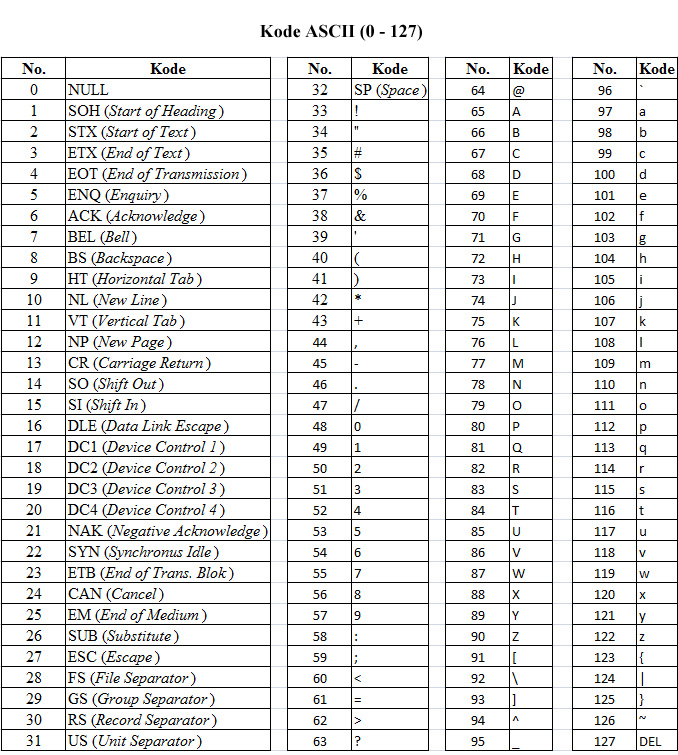
\includegraphics[width=14cm]{ASCIIreguler}
% \end{figure}
%-----------------------------------------------------------------
%-----------------------------------------------------------------
\end{document}
